% !TEX program = xelatex
\documentclass[UTF8,fontset=fandol,a4paper,11pt]{ctexart}
\usepackage[margin=21mm,top=23mm,bottom=22mm,headheight=16pt]{geometry}
\usepackage{amsmath,amssymb,mathtools,bm}
\usepackage{tikz}
\usetikzlibrary{arrows.meta,calc,angles,quotes,patterns}
\usepackage{xcolor,booktabs,array,longtable,enumitem,fancyhdr,needspace}
\usepackage[unicode,hidelinks]{hyperref}
\definecolor{ink}{HTML}{24343C}
\definecolor{accent}{HTML}{166A70}
\definecolor{muted}{HTML}{65747A}
\definecolor{rulegray}{HTML}{D4DDE0}
\definecolor{warm}{HTML}{966037}
\color{ink}
\setlength{\parindent}{2em}
\setlength{\parskip}{4pt}
\linespread{1.12}
\AtBeginDocument{\setlength{\abovedisplayskip}{6pt plus 2pt minus 1pt}
\setlength{\belowdisplayskip}{6pt plus 2pt minus 1pt}
\setlength{\abovedisplayshortskip}{0pt plus 1pt}
\setlength{\belowdisplayshortskip}{4pt plus 1pt}}
\setlist[enumerate]{label=(\arabic*),leftmargin=2.3em,itemsep=3pt,topsep=4pt}
\setlist[itemize]{leftmargin=2em,itemsep=2pt,topsep=4pt}
\allowdisplaybreaks[1]
\setlength{\emergencystretch}{2em}
\setcounter{secnumdepth}{0}
\providecommand{\tightlist}{\setlength{\itemsep}{0pt}\setlength{\parskip}{0pt}}
\ctexset{section={format=\Large\bfseries\color{accent},beforeskip=10pt,afterskip=9pt},
subsection={format=\normalsize\bfseries\color{accent},beforeskip=10pt,afterskip=4pt},
subsubsection={format=\normalsize\bfseries,beforeskip=8pt,afterskip=3pt}}
\pagestyle{fancy}
\fancyhf{}
\fancyhead[L]{\small\color{muted}物理学难题集萃}
% 页眉仅保留书名；版本名称只在封面显示。
\fancyfoot[L]{\small\color{muted}\chapterlabel}
\fancyfoot[R]{\small\thepage}
\renewcommand{\headrulewidth}{0.4pt}
\renewcommand{\footrulewidth}{0pt}
\newcommand{\dd}{\mathop{}\!\mathrm{d}}
\newcommand{\vect}[1]{\bm{#1}}
\newcommand{\tagline}[1]{\noindent{\small\color{muted}#1}\par}
\newcommand{\result}[1]{\begin{equation*}\boxed{#1}\end{equation*}}
\newcommand{\figcaption}[1]{\par\vspace{2pt}{\small\color{muted}#1}\par}
\newcommand{\teach}[2]{\Needspace{4\baselineskip}\subsection*{讲解要点与追问}#1\par\smallskip\noindent\textbf{追问：}#2\par}
\newcommand{\workarea}{\par\vspace{7mm}\noindent{\small\color{muted}作答区}\par\vspace{4mm}
\noindent\textcolor{rulegray}{\rule{\linewidth}{0.3pt}}\par\vspace{16mm}
\noindent\textcolor{rulegray}{\rule{\linewidth}{0.3pt}}\par\vspace{16mm}
\noindent\textcolor{rulegray}{\rule{\linewidth}{0.3pt}}\par\vspace{16mm}
\noindent\textcolor{rulegray}{\rule{\linewidth}{0.3pt}}}
\tikzset{axis/.style={-{Stealth[length=2mm]},thin,color=muted},
motion/.style={-{Stealth[length=2.3mm]},thick,color=accent},
force/.style={-{Stealth[length=2.3mm]},thick,color=warm},
traj/.style={thick,color=accent},guide/.style={dashed,thin,color=muted},
object/.style={thick,color=ink},every node/.style={font=\small}}\widowpenalty=10000\clubpenalty=10000\displaywidowpenalty=10000\newcommand{\chapterlabel}{电磁学第二章\quad 磁场、磁介质}

\hypersetup{pdftitle={电磁学第二章 磁场、磁介质·学生解答版},pdfauthor={}}

\begin{document}

\pdfbookmark[0]{电磁学第二章 磁场、磁介质}{cover}

\thispagestyle{empty}\vspace*{22mm}
\noindent{\Huge\bfseries 物理学难题集萃}\par\vspace{10mm}
\noindent{\LARGE 电磁学第二章}\par\vspace{6mm}
\noindent{\LARGE 磁场、磁介质}\par\vspace{12mm}
\noindent{\Large\color{accent}学生解答版}\par\vspace{9mm}
\noindent\textcolor{accent}{\rule{\linewidth}{1pt}}\par\vspace{9mm}
\noindent 第1--27题\par\vfill\clearpage
\pdfbookmark[1]{题目目录}{contents}\section*{题目目录}
\begin{longtable}{@{}r p{113mm} r@{}}\toprule 题号 & 题目 & 页码\\\midrule

\hyperref[q:1]{1} & \hyperref[q:1]{半球面经线电流的球心磁场} & \pageref{q:1} \\

\hyperref[q:2]{2} & \hyperref[q:2]{抛物线形电流在焦点的磁场} & \pageref{q:2} \\

\hyperref[q:3]{3} & \hyperref[q:3]{均匀带电球面旋转的轴内磁场} & \pageref{q:3} \\

\hyperref[q:4]{4} & \hyperref[q:4]{无限长螺旋导线的轴上磁场} & \pageref{q:4} \\

\hyperref[q:5]{5} & \hyperref[q:5]{互补圆柱导体空隙中的均匀磁场} & \pageref{q:5} \\

\hyperref[q:6]{6} & \hyperref[q:6]{有限厚电流层的磁场分布} & \pageref{q:6} \\

\hyperref[q:7]{7} & \hyperref[q:7]{载流圆柱内的电子收缩与净电荷} & \pageref{q:7} \\

\hyperref[q:8]{8} & \hyperref[q:8]{磁场中转杆与滑动带电环} & \pageref{q:8} \\

\hyperref[q:9]{9} & \hyperref[q:9]{地磁场中带电圆环的滑动与纯滚动} & \pageref{q:9} \\

\hyperref[q:10]{10} & \hyperref[q:10]{电子枪击靶的圆轨道与螺旋轨道} & \pageref{q:10} \\

\hyperref[q:11]{11} & \hyperref[q:11]{平移细管内出射粒子追碰目标} & \pageref{q:11} \\

\hyperref[q:12]{12} & \hyperref[q:12]{方波轴向磁场中的电子束聚焦} & \pageref{q:12} \\

\hyperref[q:13]{13} & \hyperref[q:13]{同轴磁控管的临界磁场} & \pageref{q:13} \\

\hyperref[q:14]{14} & \hyperref[q:14]{点源到点像的磁场边界} & \pageref{q:14} \\

\hyperref[q:15]{15} & \hyperref[q:15]{电子束先会聚再扩束的四区磁场} & \pageref{q:15} \\

\hyperref[q:16]{16} & \hyperref[q:16]{环形磁场中的电子束聚焦与漂移} & \pageref{q:16} \\

\hyperref[q:17]{17} & \hyperref[q:17]{磁铁边缘场的单平面聚焦} & \pageref{q:17} \\

\hyperref[q:18]{18} & \hyperref[q:18]{电场漂移与磁场梯度漂移} & \pageref{q:18} \\

\hyperref[q:19]{19} & \hyperref[q:19]{重力与磁场中同高度的再相遇} & \pageref{q:19} \\

\hyperref[q:20]{20} & \hyperref[q:20]{载流双杆与弹簧的小振动} & \pageref{q:20} \\

\hyperref[q:21]{21} & \hyperref[q:21]{旋转带电圆环的附加张力} & \pageref{q:21} \\

\hyperref[q:22]{22} & \hyperref[q:22]{圆电流对共面长直导线的作用力} & \pageref{q:22} \\

\hyperref[q:23]{23} & \hyperref[q:23]{闭合稳恒电流回路间的作用与反作用} & \pageref{q:23} \\

\hyperref[q:24]{24} & \hyperref[q:24]{超导平板上方电流环的悬浮与振动} & \pageref{q:24} \\

\hyperref[q:25]{25} & \hyperref[q:25]{均匀磁化长棒侧面的场边界} & \pageref{q:25} \\

\hyperref[q:26]{26} & \hyperref[q:26]{均匀磁化球壳在球心的磁场} & \pageref{q:26} \\

\hyperref[q:27]{27} & \hyperref[q:27]{旋转径向极化圆柱的场能量} & \pageref{q:27} \\

\bottomrule\end{longtable}

\noindent 本章采用SI单位。$e>0$为电子电荷的绝对值，电子电荷为$-e$。图中$\odot$表示垂直纸面向外，$\otimes$表示垂直纸面向里；近似范围与其余符号在各题中说明。

\clearpage

\pdfbookmark[2]{第 1 题 半球面经线电流的球心磁场}{q1}

\section*{第 1 题\quad 半球面经线电流的球心磁场}\label{q:1}

半径为$R$的金属球面上，电流$2I$由南极流入、沿经线均匀分布后在北极流出，两端接沿极轴延伸的半无限长直导线。现沿过极轴的平面把球分成左右两半，移去右半球面；余下左半球面的电流分布保持不变，总电流为$I$。取极轴为$z$轴，左半球位于$y<0$，$x,y,z$构成右手坐标系。求球心$O$处的磁感应强度。

\begin{center}\begin{minipage}{.97\linewidth}\centering
\begin{tikzpicture}[x=1cm,y=1cm,font=\small]
\fill[accent!10] (0,-1.7) arc(-90:-270:1.7)--cycle;
\draw[object] (0,-1.7) arc(-90:-270:1.7);
\draw[guide] (0,-1.7)--(0,1.7);
\draw[axis] (0,0)--(2.7,0) node[right] {$y$};
\draw[axis] (0,0)--(0,2.85) node[above] {$z$};
\draw[motion] (0,-2.6)--(0,-1.75) node[midway,right] {$I$};
\draw[motion] (0,1.75)--(0,2.6) node[midway,right] {$I$};
\draw[motion] (-1.62,-.48) arc(-163:-197:1.7);
\node[left] at (-1.8,0) {$I:\ \mathrm S\to\mathrm N$};
\fill (0,0) circle(1.5pt) node[below right] {$O$};
\draw[<->] (0,0)--(-1.2,1.2) node[midway,above] {$R$};
\node at (1.8,-1.05) {$\odot\ +x$};
\node at (-.6,-2.95) {$yz$截面，保留$y<0$半球};
\end{tikzpicture}
\figcaption{图电2.1　过极轴的截面；箭头表示南极到北极的经线电流。切面为$y=0$，极轴两端接线均在球外。}
\end{minipage}\end{center}


\Needspace{6\baselineskip}\subsection*{解答}

图电2.1中，接线在极轴上，任意接线元到$O$的位矢与电流元平行，所以$\dd\vect l\times\vect r=0$，接线不贡献球心磁场。把半球按经线方位角分成细条，每条从南极连到北极，都是半径$R$的半圆电流。

\begin{center}\begin{minipage}{.97\linewidth}\centering
\begin{tikzpicture}[x=1cm,y=1cm,font=\small]
\draw[axis] (-2.1,0)--(2.5,0) node[right] {$y$};
\draw[axis] (0,-2)--(0,2.1) node[above] {$x$};
\draw[object] (0,-1.6) arc(-90:-270:1.6);
\coordinate (O) at (0,0);
\fill (O) circle(1.4pt) node[above right] {$O$};
\coordinate (M) at (-1.131,-1.131);
\coordinate (N) at (-1.131,1.131);
\draw[guide] (O)--(M) node[below left] {$\theta$经线};
\draw[guide] (O)--(N) node[above left] {$\pi-\theta$经线};
\draw (0,-.48) arc(-90:-135:.48);
\node at (-.32,-.69) {$\theta$};
\draw[force] (O)--(.95,-.95) node[right] {$\mathrm d\boldsymbol B_\theta$};
\draw[force] (O)--(-.95,-.95) node[left] {$\mathrm d\boldsymbol B_{\pi-\theta}$};
\draw[motion] (O)--(0,-1.9) node[right] {合场沿$-x$};
\node[align=left] at (4.8,.8) {$\boldsymbol n=( -\cos\theta,-\sin\theta,0)$\\
$\mathrm d\boldsymbol B\parallel-\boldsymbol e_z\times\boldsymbol n$\\
$\mathrm d B_x=-\mathrm dB\sin\theta$\\
$\mathrm d B_y=\mathrm dB\cos\theta$};
\end{tikzpicture}
\figcaption{解图电2.1A　从$-x$向$-y$再到$+x$定义$0\le\theta\le\pi$。箭头都从O出发；配对后$y$分量抵消，$-x$分量相加。}
\end{minipage}\end{center}


解图电2.1A以$\theta\in[0,\pi]$标记经线平面，角度从$-x$端量起。原来全球总电流$2I$按$2\pi$方位均分，故细条中
\[
 \dd I=\frac{2I}{2\pi}\dd\theta=\frac I\pi\dd\theta.
\]
毕奥—萨伐尔定律给出半圆在圆心的磁场
\[
 \dd B=\frac{\mu_0\dd I}{4R}=\frac{\mu_0 I}{4\pi R}\dd\theta.
\]

在半球中间的经线取赤道附近的电流元来确定场方向：它沿$+z$，源点到$O$沿$+y$，故$\dd\vect l\times\vect r$沿$-x$。半圆上其余元的场同向，因此解图电2.1A的负$x$投影与真实电流方向一致。各细条电流满足$\int_0^\pi\dd I=I$，也与剩余半球的总量相符。

\Needspace{12\baselineskip}
按右手定则，各细条的场都在$xy$平面。关于半球中间经线对称的两条，$y$分量抵消，负$x$分量相加。按图的角度定义，$\dd B_x=-\dd B\sin\theta$，于是
\[
 B_x=-\frac{\mu_0 I}{4\pi R}\int_0^\pi\sin\theta\dd\theta
 =-\frac{\mu_0 I}{2\pi R},\qquad B_y=B_z=0.
\]
\result{\vect B(O)=-\frac{\mu_0 I}{2\pi R}\vect e_x.}
保留半球有向负 $x$ 的合场。完整球面上，跨过同一直径的两条经线赤道位置相反，半圆场也相反，逐对相加为零。

解图电2.1A把角度零点固定在赤道的$-x$端。若经线赤道位置的单位矢量为
\[
\boldsymbol n=-\cos\theta\,\boldsymbol e_x-\sin\theta\,\boldsymbol e_y,
\]
南极到北极的电流在该经线赤道处沿$+\boldsymbol e_z$，到O的位矢沿$-\boldsymbol n$，所以半圆场的单位方向为
\[
-\boldsymbol e_z\times\boldsymbol n
=-\sin\theta\,\boldsymbol e_x+\cos\theta\,\boldsymbol e_y.
\]
A图的两条场箭头按这两个分量同时绘制，角度零点和投影符号由此对应。
解图电2.1B选中间经线的真实电流元：向上的电流与向右的位矢叉乘，给出朝纸内的$-x$方向。

\begin{center}\begin{minipage}{.97\linewidth}\centering
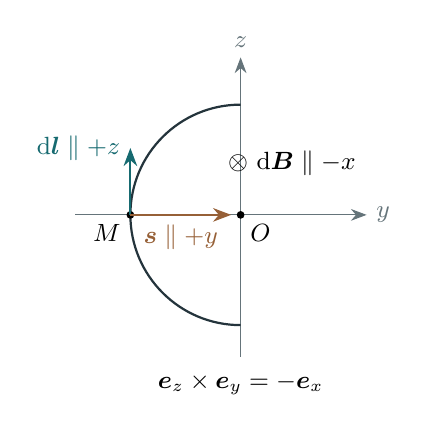
\begin{tikzpicture}[x=1cm,y=1cm,font=\small]
\draw[axis] (-2.1,0)--(1.6,0) node[right] {$y$};
\draw[axis] (0,-1.8)--(0,2) node[above] {$z$};
\draw[object] (0,-1.4) arc(-90:-270:1.4);
\fill (0,0) circle(1.4pt) node[below right] {$O$};
\fill (-1.4,0) circle(1.4pt) node[below left] {$M$};
\draw[motion] (-1.4,0)--(-1.4,.85) node[left] {$\mathrm d\boldsymbol l\parallel+z$};
\draw[force] (-1.4,0)--(-.12,0) node[midway,below] {$\boldsymbol s\parallel+y$};
\node at (.65,.65) {$\otimes\ \mathrm d\boldsymbol B\parallel-x$};
\node at (0,-2.15) {$\boldsymbol e_z\times\boldsymbol e_y=-\boldsymbol e_x$};
\end{tikzpicture}
\figcaption{解图电2.1B　取 $x=0,y=-R$ 处的电流元；图中 $+x$ 朝纸外，磁场朝纸内。}
\end{minipage}\end{center}

把角分配写成面电流密度，可以看清同一条细带怎样沿纬度传递电流。令$\vartheta$为从北极量起的极角，与方位角$\theta$不同。
在纬度$\vartheta$处，一条细带的横向宽度是$R\sin\vartheta\,\mathrm d\theta$；其面电流密度$K$满足
\[
\mathrm dI=K(\vartheta)R\sin\vartheta\,\mathrm d\theta
=\frac I\pi\,\mathrm d\theta,\qquad
K(\vartheta)=\frac{I}{\pi R\sin\vartheta}.
\]
\begin{center}\begin{minipage}{.97\linewidth}\centering
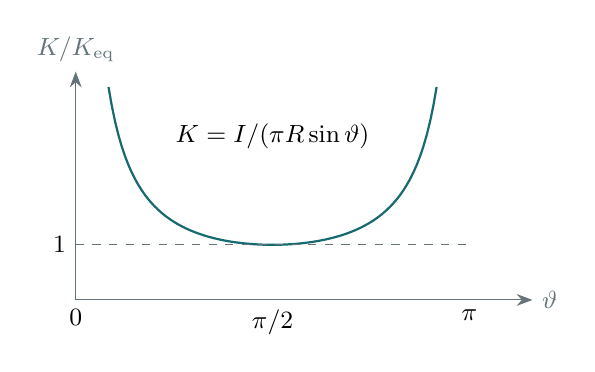
\begin{tikzpicture}[x=1cm,y=1cm,font=\small]
\draw[axis] (0,0)--(5.8,0) node[right] {$\vartheta$};
\draw[axis] (0,0)--(0,2.9) node[above] {$K/K_{\rm eq}$};
\draw[traj,domain=15:165,samples=100] plot ({5*\x/180},{.7/sin(\x)});
\draw[guide] (0,.7)--(5,.7);
\node[left] at (0,.7) {$1$};
\node[below] at (0,0) {$0$};\node[below] at (2.5,0) {$\pi/2$};\node[below] at (5,0) {$\pi$};
\node[above] at (2.5,1.8) {$K=I/(\pi R\sin\vartheta)$};
\end{tikzpicture}
\figcaption{解图电2.1C　经线面电流密度在两极附近增大；曲线只画远离极点的部分。每条细带的电流仍为$I\,\mathrm d\theta/\pi$。}
\end{minipage}\end{center}

解图电2.1C中的$K$并不处处相同；赤道值$K_{\rm eq}=I/(\pi R)$最小，两极的理想化发散来自电流汇入和流出同一点。
越靠近极点，细带宽度越小、面电流密度越大，两者相乘仍为同一细带电流。对任一纬圈在保留半球上的半周积分，
\[
\int_0^\pi K R\sin\vartheta\,\mathrm d\theta=I.
\]
稳恒条件固定的是穿过纬圈的总电流，因此面电流密度随纬圈半径按反比变化。


\Needspace{18\baselineskip}

\pdfbookmark[2]{第 2 题 抛物线形电流在焦点的磁场}{q2}

\section*{第 2 题\quad 抛物线形电流在焦点的磁场}\label{q:2}

一根无限长细导线弯成抛物线，焦点到顶点的距离为$a$，通有恒定电流$I$。取抛物线为$x^2=4ay$，焦点$P=(0,a)$，电流从左支流向顶点，再沿右支流出。求$P$处的磁感应强度。

\begin{center}\begin{minipage}{.98\linewidth}\centering
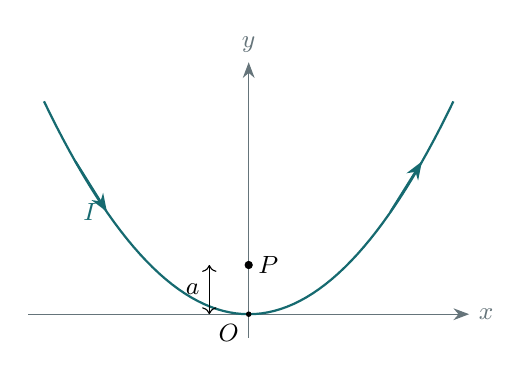
\begin{tikzpicture}[x=1cm,y=1cm]
\draw[axis] (-2.8,0)--(2.8,0) node[right] {$x$};\draw[axis] (0,-.3)--(0,3.2) node[above] {$y$};\draw[traj,domain=-2.6:2.6,samples=65] plot(\x,{.4*\x*\x});
\fill (0,0) circle(1pt) node[below left] {$O$};\fill (0,.625) circle(1.5pt) node[right] {$P$};\draw[<->] (-.5,0)--(-.5,.625) node[midway,left] {$a$};\draw[motion] (-2.2,1.94)--(-1.8,1.3) node[left] {$I$};\draw[motion] (1.8,1.3)--(2.2,1.94);
\end{tikzpicture}\figcaption{图电2.2　电流沿左支向下、右支向上。}\end{minipage}\end{center}

\Needspace{6\baselineskip}\subsection*{解答}

解图电2.2A在右支取电流元，按电流方向以$x$为参数，$x$从$-\infty$增至$+\infty$。电流元位置$(x,y)$，到焦点的位矢为
\[
 \vect s=-x\vect e_x+(a-y)\vect e_y,\qquad
 \dd\vect l=\dd x\vect e_x+\dd y\vect e_y.
\]
\begin{center}\begin{minipage}{.98\linewidth}\centering
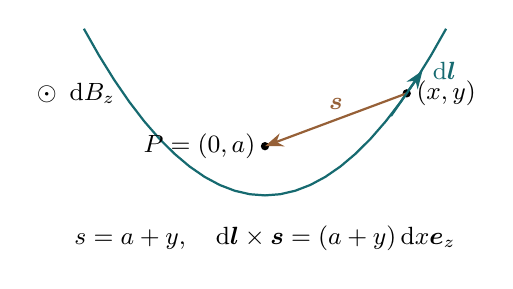
\begin{tikzpicture}[x=1cm,y=1cm]
\draw[traj,domain=-2.3:2.3] plot(\x,{.4*\x*\x});\fill (0,.625) circle(1.5pt) node[left] {$P=(0,a)$};\fill (1.8,1.296) circle(1.5pt) node[right] {$(x,y)$};\draw[force] (1.8,1.296)--(0,.625) node[midway,above] {$\vect s$};\draw[motion] (1.6,1.008)--(2,1.584) node[right] {$\dd\vect l$};\node at (-2.4,1.3) {$\odot\ \dd B_z$};\node at (0,-.55) {$s=a+y,\quad \dd\vect l\times\vect s=(a+y)\dd x\vect e_z$};
\end{tikzpicture}\figcaption{解图电2.2A　电流元到焦点的距离和叉乘均可用a+y表示。}\end{minipage}\end{center}
由$y=x^2/(4a)$，有$y'=x/(2a)$，因而
\[
 \dd\vect l\times\vect s
 =[a-y+xy']\dd x\vect e_z=(a+y)\dd x\vect e_z.
\]
这里$\vect e_z$垂直纸面向外。抛物线的焦点距离满足
\[
 s^2=x^2+(a-y)^2=4ay+(a-y)^2=(a+y)^2,
 \qquad s=a+y>0.
\]
所以所有电流元的磁场均沿正$z$方向，且
\[
 \dd B_z=\frac{\mu_0 I}{4\pi}\frac{(a+y)\dd x}{s^3}
 =\frac{\mu_0 I}{4\pi a^2}\frac{\dd x}{[1+(x/2a)^2]^2}.
\]
左右两支的被积函数相同。令$x=2a\tan\alpha$，$\dd x=2a\sec^2\alpha\dd\alpha$，则
\[
 B_z=\frac{\mu_0 I}{2\pi a^2}\int_0^\infty\frac{\dd x}{[1+(x/2a)^2]^2}
 =\frac{\mu_0 I}{\pi a}\int_0^{\pi/2}\cos^2\alpha\dd\alpha
 =\frac{\mu_0 I}{4a}.
\]

\Needspace{14\baselineskip}
以切线倾角 $\alpha$ 为变量，正半支的 $x:0\to\infty$ 对应 $\alpha:0\to\pi/2$，并有
\[\frac{\dd x}{[1+(x/2a)^2]^2}
=\frac{2a\sec^2\alpha\dd\alpha}{\sec^4\alpha}
=2a\cos^2\alpha\dd\alpha.\]
解图电2.2A中每个电流元的叉乘分子为 $a+y>0$。左右两支上的电流都沿 $x$ 增加的方向，且互为镜像的两点有相同 $y$，所以给相等、同向的磁场微元。

这里的最后一个积分可直接展开：
\[
 \int_0^{\pi/2}\cos^2\alpha\,\dd\alpha
 =\left[\frac{\alpha}{2}+\frac{\sin2\alpha}{4}\right]_0^{\pi/2}
 =\frac{\pi}{4}.
\]
全轴积分化成两倍正半轴积分的因子已经计在前面的系数中。

\result{\vect B(P)=\frac{\mu_0 I}{4a}\vect e_z.}
反向通电时方向反转；整个计算中的$a$是焦距，若使用方程$x^2=2py$，应先代入$p=2a$。

解图电2.2B给出$s=a+y$的几何解释：焦点到曲线上 M 的距离，等于 M 到准线 $y=-a$ 的距离。
焦点与准线是这一定义中的配对对象。若改用场点 $(0,2a)$，其距离应写成 $\sqrt{x^2+(2a-y)^2}$，按新核积分。
同时，切线斜率$y'=x/(2a)$给$\tan\alpha=x/(2a)$，所以积分中的三角换元正好使用切线倾角。
图中示例$x=2a$给$\alpha=\pi/4$、$y=a$、$s=2a$，此时到焦点的距离与到水平准线的距离都为 $2a$。
\begin{center}\begin{minipage}{.97\linewidth}\centering
\begin{tikzpicture}[x=1.6cm,y=1.6cm,font=\small]
\draw[axis] (-1.8,0)--(2.7,0) node[right] {$x$};
\draw[axis] (0,-.95)--(0,2) node[above] {$y$};
\draw[traj,domain=-1.7:1.7,samples=70] plot(\x,{.4*\x*\x});
\draw[guide] (-1.8,-.625)--(2.5,-.625) node[right] {准线$y=-a$};
\coordinate (M) at (1.25,.625);\coordinate (P) at (0,.625);\coordinate (N) at (1.25,-.625);
\fill (P) circle(1.4pt) node[left] {$P$};
\fill (M) circle(1.4pt) node[below right] {$M$};
\draw[force] (M)--(P) node[midway,above=6pt] {$s=a+y$};
\draw[guide] (M)--(N) node[pos=.72,right] {$a+y$};
\draw[object] (1.25,-.49)--(1.12,-.49)--(1.12,-.625);
\draw[motion] (M)--(1.85,1.225) node[above] {切线};
\draw[guide] (M)--(2.05,.625);
\draw (1.6,.625) arc(0:45:.35);
\node at (1.83,.84) {$\alpha$};
\node[below right] at (0,0) {$O$};
\node[below] at (1.25,-.625) {$N$};
\end{tikzpicture}
\figcaption{解图电2.2B　示例取$x=2a$；焦点距离MP等于到准线的距离MN。切线倾角满足$\tan\alpha=x/(2a)$。}
\end{minipage}\end{center}

解图电2.2C显示每一段对全积分的贡献。只计算$|x|\le X$的导线段，令$u=X/(2a)\ge0$，则
\[
G(u)=\arctan u+\frac{u}{1+u^2},\qquad
B(X)=\frac{\mu_0I}{2\pi a}G(u).
\]
这是该段的场；连接两端所需导线的贡献须按其实际位置另计，或明确使其远离焦点。
\begin{center}\begin{minipage}{.97\linewidth}\centering
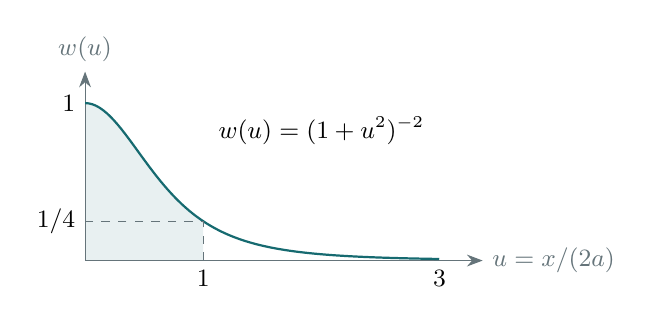
\begin{tikzpicture}[x=1cm,y=1cm,font=\small]
\fill[accent!10] (0,0)--plot[domain=0:1,samples=50] ({1.5*\x},{2/(1+\x*\x)^2})--(1.5,0)--cycle;
\draw[axis] (0,0)--(5.05,0) node[right] {$u=x/(2a)$};
\draw[axis] (0,0)--(0,2.4) node[above] {$w(u)$};
\draw[traj,domain=0:3,samples=100] plot({1.5*\x},{2/(1+\x*\x)^2});
\draw[guide] (1.5,0)--(1.5,.5)--(0,.5);
\node[left] at (0,2) {$1$};\node[left] at (0,.5) {$1/4$};
\node[below] at (1.5,0) {$1$};\node[below] at (4.5,0) {$3$};
\node[above] at (3,1.35) {$w(u)=(1+u^2)^{-2}$};
\end{tikzpicture}
\figcaption{解图电2.2C　正半支的真实无量纲积分核。阴影对应$0\le x\le2a$；两支按同一范围截取后，磁场占全导线约81.8\%。}
\end{minipage}\end{center}

由解图电2.2C的面积，保留中央$|x|\le2a$时，
\[
\frac{B(2a)}{B(\infty)}
=\frac2\pi\left(\frac\pi4+\frac12\right)
=\frac12+\frac1\pi\simeq0.8183.
\]
远处的核按 $u^{-4}$ 下降，沿尾部积分后得到三次倒数的首项：
\[
1-\frac{B(X)}{B(\infty)}
=\frac4{3\pi u^3}+O(u^{-5}),\qquad u\gg1.
\]
C图中的核处处为正；各段的场都沿$+z$，截短只减小大小，方向保持不变。

\Needspace{18\baselineskip}

\pdfbookmark[2]{第 3 题 均匀带电球面旋转的轴内磁场}{q3}

\section*{第 3 题\quad 均匀带电球面旋转的轴内磁场}\label{q:3}

半径$R$、面电荷密度$\sigma$的均匀带电球面，绕一条直径以角速度$\vect\omega=\omega\vect e_x$匀速旋转。证明：球内该直径上各点的磁感应强度相同，并求其值。

\begin{center}\begin{minipage}{.98\linewidth}\centering
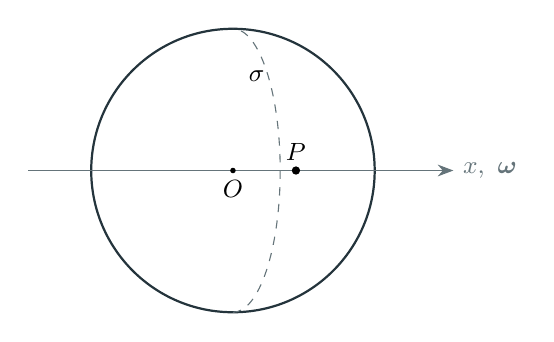
\begin{tikzpicture}[x=1cm,y=1cm]
\draw[object] (0,0) circle(1.8);\draw[axis] (-2.6,0)--(2.8,0) node[right] {$x,\ \vect\omega$};\draw[guide] (0,-1.8) arc(-90:90:.6 and 1.8);\fill (0,0) circle(1pt) node[below] {$O$};\node at (.3,1.2) {$\sigma$};\fill (.8,0) circle(1.5pt) node[above] {$P$};
\end{tikzpicture}\figcaption{图电2.3　旋转轴取水平x轴，P位于球内轴段。}\end{minipage}\end{center}

\Needspace{6\baselineskip}\subsection*{解答}

把解图电2.3A中的球面按垂直$x$轴的平面切成圆环。环中心坐标为$x$，环半径$s=\sqrt{R^2-x^2}$。取相邻两平面之间轴向坐标的正间距为 $\dd x$。球带沿子午线的宽度为 $R|\dd\phi|$，其中 $x=R\cos\phi$、$s=R\sin\phi$。因此
\[
 \dd S=2\pi sR|\dd\phi|=2\pi R\dd x,
 \qquad \dd I=\frac{\sigma\dd S}{2\pi/\omega}=\sigma R\omega\dd x.
\]
这里 $\dd I$ 的符号由 $\sigma$ 决定。

\begin{center}\begin{minipage}{.98\linewidth}\centering
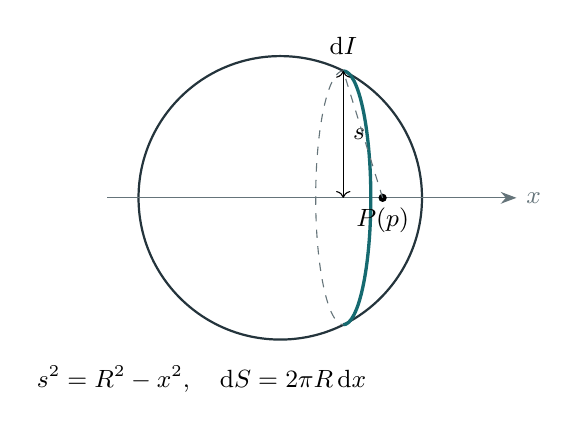
\begin{tikzpicture}[x=1cm,y=1cm]
\draw[object] (0,0) circle(1.8);\draw[axis] (-2.2,0)--(3,0) node[right] {$x$};\draw[very thick,accent] (.8,-1.612) arc(-90:90:.35 and 1.612);\draw[guide] (.8,1.612) arc(90:270:.35 and 1.612);\draw[<->] (.8,0)--(.8,1.612) node[midway,right] {$s$};\fill (1.3,0) circle(1.5pt) node[below] {$P(p)$};\node[above] at (.8,1.7) {$\dd I$};\draw[guide] (1.3,0)--(.8,1.612);\node at (-1,-2.3) {$s^2=R^2-x^2,\quad \dd S=2\pi R\dd x$};
\end{tikzpicture}\figcaption{解图电2.3A　取位于x处的旋转圆环，计算其在轴上$P(p)$处的场。}\end{minipage}\end{center}

在轴上$P=(p,0,0)$，圆环场的横向分量抵消。用递增的$x$作积分变量，得
\[
 B_x(p)=\frac{\mu_0\sigma R\omega}{2}
 \int_{-R}^{R}\frac{R^2-x^2}{(R^2+p^2-2px)^{3/2}}\dd x.
\]
积分分子 $R^2-x^2$ 来自各圆环半径的平方。对$0<|p|<R$，令$u=R^2+p^2-2px$、$A=R^2+p^2$，积分可写为
\[
 \int\frac{R^2-x^2}{u^{3/2}}\dd x
 =-\frac1{8p^3}\left[
 2(R^2-p^2)^2u^{-1/2}+4A u^{1/2}-\frac23u^{3/2}\right].
\]
\Needspace{12\baselineskip}

把方括号中的表达式记为$G(u)$。对应$x=R,-R$的$u$分别为$(R-p)^2,(R+p)^2$。取$|p|<R$，两个根号都是$R\mp p$，故三项的端点差分别给
\begin{align*}
G((R-p)^2)-G((R+p)^2)
&=4p(R^2-p^2)-8p(R^2+p^2)\\
&\quad+4R^2p+\frac43p^3
=-\frac{32}{3}p^3 .
\end{align*}
再乘原函数系数$-1/(8p^3)$，一般$p\ne0$的定积分确为$4/3$。这一步展示了位置参数怎样消去。

在$p=0$，直接积分也得
\[
 \int_{-R}^R\frac{R^2-x^2}{R^3}\dd x=\frac43.
\]
\result{\vect B(P)=\frac23\mu_0\sigma R\vect\omega,\qquad |p|<R.}
结论与$p$无关。球内还可由均匀磁化球的等效面电流得到同一均匀场，但上述圆环积分不依赖这一结论。下面改变端点根号的取值，单独求球外的轴上场。

解图电2.3B把端点取支单独画出。平方根首先是$|R-p|$、$|R+p|$；
只有$|p|<R$时，它们才能同时写成$R-p$、$R+p$。这正是上面端点差抵消位置参数的条件。
轴上各点与球心得到相同的场值，源于圆环积分的端点差。每个圆环仍用图A 所示的实际半径 $s$，满足 $s^2=R^2-x^2$。
\begin{center}\begin{minipage}{.97\linewidth}\centering
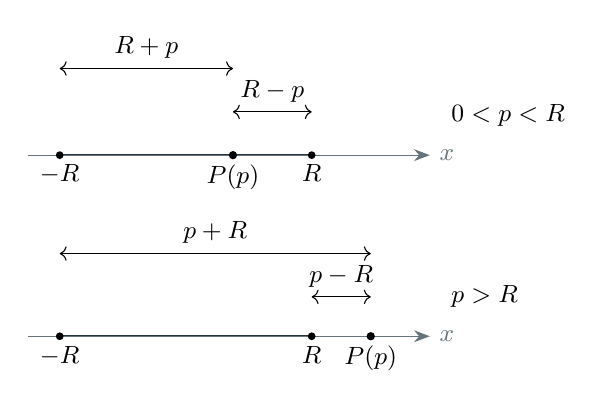
\begin{tikzpicture}[x=1cm,y=1cm,font=\small]
\foreach \h in {0,-2.3}{
\draw[object] (-1.6,\h)--(1.6,\h);
\draw[axis] (-2,\h)--(3.1,\h) node[right] {$x$};
\fill (-1.6,\h) circle(1.4pt) node[below] {$-R$};
\fill (1.6,\h) circle(1.4pt) node[below] {$R$};
}
\fill (.6,0) circle(1.5pt) node[below] {$P(p)$};
\draw[<->] (.6,.55)--(1.6,.55) node[midway,above] {$R-p$};
\draw[<->] (-1.6,1.1)--(.6,1.1) node[midway,above] {$R+p$};
\node[right] at (3.25,.5) {$0<p<R$};
\fill (2.35,-2.3) circle(1.5pt) node[below] {$P(p)$};
\draw[<->] (1.6,-1.8)--(2.35,-1.8) node[midway,above] {$p-R$};
\draw[<->] (-1.6,-1.25)--(2.35,-1.25) node[midway,above] {$p+R$};
\node[right] at (3.25,-1.8) {$p>R$};
\end{tikzpicture}
\figcaption{解图电2.3B　两个端点到轴上P的距离。根号给出绝对值；跨过右端球面后，$|R-p|$ 从 $R-p$ 改为 $p-R$。}
\end{minipage}\end{center}

沿用这一原函数算球外。先取$p>R$，将端点根号改为$p-R$、$p+R$后，
\[
G((p-R)^2)-G((p+R)^2)=-\frac{32}{3}R^3,\qquad
\mathcal I(p)=\frac{4R^3}{3p^3}.
\]
积分核在同时变换$x\to-x,p\to-p$时不变，所以$\mathcal I(-p)=\mathcal I(p)$。
整个轴线的结果因此为
\[
\boldsymbol B(p)=B_0\boldsymbol e_x
\begin{cases}
1,& |p|<R,\\[2pt]
(R/|p|)^3,& |p|>R,
\end{cases}
\qquad B_0=\frac23\mu_0\sigma R\omega.
\]
\begin{center}\begin{minipage}{.97\linewidth}\centering
\begin{tikzpicture}[x=1cm,y=1cm,font=\small]
\fill[accent!8] (-1.2,0) rectangle (1.2,1.8);
\draw[axis] (-3.4,0)--(3.5,0) node[right] {$u=p/R$};
\draw[axis] (0,0)--(0,2.25) node[above] {$B_x/B_0$};
\draw[traj,domain=-2.5:-1,samples=70] plot ({1.2*\x},{1.6/abs(\x)^3});
\draw[traj] (-1.2,1.6)--(1.2,1.6);
\draw[traj,domain=1:2.5,samples=70] plot ({1.2*\x},{1.6/\x^3});
\draw[guide] (-1.2,0)--(-1.2,1.6) (1.2,0)--(1.2,1.6);
\node[above left] at (0,1.6) {$1$};
\node[below] at (-1.2,0) {$-1$};\node[below] at (1.2,0) {$1$};
\node at (.6,.55) {轴内};
\node[above] at (-2.1,.65) {$|u|^{-3}$};
\node[above] at (2.1,.65) {$u^{-3}$};
\end{tikzpicture}
\figcaption{解图电2.3C　整个轴线的真实场，$B_0=2\mu_0\sigma R\omega/3$。两侧轴外场均与轴内场同向，大小按距离三次倒数衰减。}
\end{minipage}\end{center}

解图电2.3C中，两侧轴外的场都与轴内场同向。负电荷或反转转向会使$B_0$变号，整条曲线相应反向。
在极点 $p=R$ 直接积分：令$t=R-x$，原积分化为
\[
\mathcal I(R)=\frac1{(2R)^{3/2}}\int_0^{2R}(2R-t)t^{-1/2}\,\mathrm dt
=\frac43.
\]
端点虽有可积的平方根奇性，总场有限；$p=-R$同理，均接上图中的平台。
这与极点处旋转速度、面电流都为零相符。球面其他位置有面电流，切向磁场的跳跃由当地 $\vect K=\sigma(\vect\omega\times R\vect n)$ 决定。

\Needspace{18\baselineskip}

\pdfbookmark[2]{第 4 题 无限长螺旋导线的轴上磁场}{q4}

\section*{第 4 题\quad 无限长螺旋导线的轴上磁场}\label{q:4}

真空中一根无限长细导线，沿半径$R$、螺距$H>0$的圆柱面绕成等距螺旋线，电流为$I$。圆柱轴为$y$轴。用参数$\phi$规定导线位置
\[
 \vect r(\phi)=(R\cos\phi,h\phi,R\sin\phi),\qquad h=H/(2\pi),
\]
电流沿$\phi$增大方向。求原点$O$处磁场的三个分量；说明轴上其他点的场怎样变化。

\begin{center}\begin{minipage}{.98\linewidth}\centering
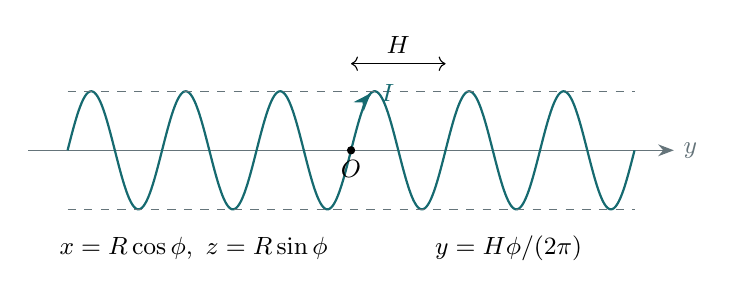
\begin{tikzpicture}[x=1cm,y=1cm]
\draw[axis] (-4.1,0)--(4.1,0) node[right] {$y$};\draw[traj,domain=-1080:1080,samples=360] plot({\x/300},{.75*sin(\x)});\draw[guide] (-3.6,.75)--(3.6,.75);\draw[guide] (-3.6,-.75)--(3.6,-.75);\draw[<->] (0,1.1)--(1.2,1.1) node[midway,above] {$H$};\fill (0,0) circle(1.5pt) node[below] {$O$};\node at (-2,-1.25) {$x=R\cos\phi,\ z=R\sin\phi$};\node at (2,-1.25) {$y=H\phi/(2\pi)$};
\draw[motion,domain=45:75,samples=12] plot({\x/300},{.75*sin(\x)}) node[right] {$I$};
\end{tikzpicture}\figcaption{图电2.4　螺旋线的投影；完整空间方位由参数式规定。}\end{minipage}\end{center}

\Needspace{6\baselineskip}\subsection*{解答}

解图电2.4A把螺旋电流元分为绕轴的圆周分量和沿轴的直线分量。相对于$O$，电流元和源点到场点的位矢分别为
\[
 \dd\vect l=(-R\sin\phi,h,R\cos\phi)\dd\phi,
 \qquad\vect s=-\vect r(\phi),\qquad s^2=R^2+h^2\phi^2.
\]
\begin{center}\begin{minipage}{.97\linewidth}\centering
\begin{tikzpicture}[x=1.5cm,y=1.5cm,font=\small]
\coordinate (O) at (0,0);
\coordinate (S) at (.6516,.9192);
\coordinate (V) at (1.3516,.9192);
\coordinate (W) at (.9733,1.5874);
\coordinate (T) at (1.6733,1.5874);
\draw[axis] (-.4,0)--(2.8,0) node[right] {$y$};
\draw[axis] (O)--(0,2.25) node[above] {$z$};
\draw[axis] (O)--(-1.2,-.65) node[below] {$x$};
\fill (S) circle(1.4pt);
\draw[guide] (S)--(-.35,1.5) node[left] {$S(\phi),\ \boldsymbol r(\phi)$};
\draw[force] (S)--(O) node[midway,left] {$\boldsymbol s$};
\draw[motion] (S)--(V) node[below right] {$\mathrm d\boldsymbol l_y$};
\draw[motion] (S)--(W) node[above left] {$\mathrm d\boldsymbol l_\phi$};
\draw[object,->] (S)--(T) node[right] {$\mathrm d\boldsymbol l$};
\draw[guide] (V)--(T)--(W);
\node[below] at (O) {$O$};
\end{tikzpicture}
\figcaption{解图电2.4A　按$\phi=\pi/4,\ R=h$的真实切向方向作投影，三个电流元箭头共起点S。直线分量沿$+y$，圆周分量在$xz$平面；两者到O的位矢相同。}
\end{minipage}\end{center}

逐分量叉乘，保留两类电流的贡献，有
\[
 \dd\vect l\times\vect s=
 \bigl(hR[\phi\cos\phi-\sin\phi],-R^2,
 hR[\phi\sin\phi+\cos\phi]\bigr)\dd\phi.
\]
为逐项追踪A图中的两个箭头，先写
\[
\mathrm d\boldsymbol l_\phi=(-R\sin\phi,0,R\cos\phi)\,\mathrm d\phi,\qquad
\mathrm d\boldsymbol l_y=(0,h,0)\,\mathrm d\phi.
\]
在同一个位置S，它们与$\boldsymbol s=(-R\cos\phi,-h\phi,-R\sin\phi)$分别叉乘：
\[
\begin{aligned}
\mathrm d\boldsymbol l_\phi\times\boldsymbol s
&=(hR\phi\cos\phi,-R^2,hR\phi\sin\phi)\,\mathrm d\phi,\\
\mathrm d\boldsymbol l_y\times\boldsymbol s
&=(-hR\sin\phi,0,hR\cos\phi)\,\mathrm d\phi.
\end{aligned}
\]
相加才是前面的总电流元叉乘。轴向分量来自圆周电流元；横向分量是圆周电流元与轴向电流元的场之和。
特别在$\phi=0$的交点，圆周电流沿$+z$、源点到O沿$-x$，叉乘给$-y$；
轴向电流沿$+y$，与同一$-x$位矢叉乘给$+z$。这个交点的两个叉乘分别给出轴向负号和横向局部正号。
\begin{center}\begin{minipage}{.97\linewidth}\centering
\begin{tikzpicture}[x=1cm,y=1.3cm,font=\small]
\draw[axis] (-4.4,0)--(4.5,0) node[right] {$\phi$};
\draw[axis] (0,-1.25)--(0,1.4) node[above] {无量纲核};
\draw[force,domain=-4:4,samples=150] plot(\x,{(\x*cos(deg(\x))-sin(deg(\x)))/(1+\x*\x)^1.5});
\draw[guide,domain=-4:4,samples=150] plot(\x,{-1/(1+\x*\x)^1.5});
\draw[traj,domain=-4:4,samples=150] plot(\x,{(\x*sin(deg(\x))+cos(deg(\x)))/(1+\x*\x)^1.5});
\node[right,warm] at (4.8,.8) {$f_x$：奇};
\node[right,muted] at (4.8,.35) {$f_y$：偶};
\node[right,accent] at (4.8,-.1) {$f_z$：偶};
\node[below=9pt] at (-3.1416,0) {$-\pi$};\node[below=9pt] at (3.1416,0) {$\pi$};
\end{tikzpicture}
\figcaption{解图电2.4B　取$R/h=1$画三分量的真实积分核。只有 $x$ 项为奇函数；偶函数 $f_z$ 包含正、负两种区间。}
\end{minipage}\end{center}

解图电2.4B对应
\[
f_x=\frac{\phi\cos\phi-\sin\phi}{(1+\phi^2)^{3/2}},\quad
f_y=-\frac1{(1+\phi^2)^{3/2}},\quad
f_z=\frac{\phi\sin\phi+\cos\phi}{(1+\phi^2)^{3/2}}.
\]
在 $\phi$ 与 $-\phi$ 处，$f_x$ 取反，$f_y$、$f_z$ 各自保持。这个奇偶性对两类电流元的 $x$ 分量分别成立。图 B 取 $R/h=1$；其他半径和螺距下分母也是偶函数。

$x$分量是奇函数，积分为零。$y$分量为
\[
 B_y=-\frac{\mu_0IR^2}{4\pi}\int_{-\infty}^{\infty}
 \frac{\dd\phi}{(R^2+h^2\phi^2)^{3/2}}
 =-\frac{\mu_0 I}{2\pi h}=-\frac{\mu_0 I}{H}.
\]

上述轴向积分中令$u=h\phi/R$，有
\[
 \int_{-\infty}^{\infty}\frac{\dd\phi}{(R^2+h^2\phi^2)^{3/2}}
 =\frac1{hR^2}
 \left[\frac{u}{\sqrt{1+u^2}}\right]_{-\infty}^{\infty}
 =\frac2{hR^2}.
\]
因此负号来自解图电2.4A所对应的绕向，系数来自全轴积分。

解图中$\dd l_\phi=R\dd\phi$、$\dd l_y=h\dd\phi$。将圆周分量均摊成圆环后，轴向场等效为每单位长度$1/H$匝的长螺线管，也可得到$B_y$；这一步只能用于轴向分量。

还可以把圆周电流元对轴向场的等效关系写完整。固定轴坐标$y=h\phi$，
圆周电流元的有向长度为$R\,\mathrm d\phi$。它到O的距离只取决于$R,y$，
而它的叉乘在轴上的$y$分量恒为$-R\,\mathrm dl_\phi$，不随绕轴方位变化。
因此，仅就这一分量，可把同一个$I\,\mathrm dl_\phi$均摊在该高度的整个圆周上。等效圆环电流满足
\[
\mathrm dI'\,2\pi R=I\,\mathrm dl_\phi,\qquad
\mathrm dI'=\frac{I\,\mathrm d\phi}{2\pi}
=\frac I H\,\mathrm dy.
\]
相邻高度$\mathrm dy$之间连续排置这样的圆环，电流与轴长之比为$I/H$。
若形式上把每段高度看作一匝，则$n=1/\mathrm dy$、每匝电流为$\mathrm dI'$，
乘积$n\,\mathrm dI'=I/H$有限。无限长螺线管的轴向场于是给出
\[
B_{1y}=-\mu_0 n\,\mathrm dI'=-\frac{\mu_0I}{H}.
\]
这与直接积分一致。上述平均没有搬动轴坐标，只消去了同一高度的方位；
算横向场时保留线元的实际方位。下面的 $B_{1z}$、$B_{2z}$ 分别来自圆周和轴向电流元。

由A图两式分别抽出$z$分量，在$s^2=R^2+h^2\phi^2$下，
\[
\begin{aligned}
\mathrm dB_{1z}
&=\frac{\mu_0I}{4\pi}\frac{hR\phi\sin\phi}{s^3}\,\mathrm d\phi,\\
\mathrm dB_{2z}
&=\frac{\mu_0I}{4\pi}\frac{hR\cos\phi}{s^3}\,\mathrm d\phi.
\end{aligned}
\]
第一式来自圆周电流与轴向距离$y=h\phi$的结合；第二式来自轴向电流元
$\mathrm dl_y=h\,\mathrm d\phi$和到轴的径向距离R，再向固定$z$轴投影。
两个核都随 $\phi$ 改变符号，局部贡献按相应的 $\sin\phi$ 和 $\cos\phi$ 取正、负。
分母变为
\[
s^3=\left(\frac H{2\pi}\right)^3
\left[\left(\frac{2\pi R}{H}\right)^2+\phi^2\right]^{3/2}.
\]
故圆周与直线两部分分别积分得
\[
\begin{aligned}
B_{1z}&=\frac{2\pi\mu_0IR}{H^2}\int_0^\infty
\frac{\phi\sin\phi}{[(2\pi R/H)^2+\phi^2]^{3/2}}\,\mathrm d\phi,\\
B_{2z}&=\frac{2\pi\mu_0IR}{H^2}\int_0^\infty
\frac{\cos\phi}{[(2\pi R/H)^2+\phi^2]^{3/2}}\,\mathrm d\phi.
\end{aligned}
\]
两行的因子2均来自偶对称，相加得到总 $B_z$。
$|\phi|\to\infty$时，第一项至多按$\phi^{-2}$、第二项按$\phi^{-3}$衰减，两个积分都绝对收敛。

上述两个 $z$ 分量的积分核均为偶函数，合并得
\[
 B_z=\frac{\mu_0IhR}{2\pi}\int_0^\infty
 \frac{\phi\sin\phi+\cos\phi}{(R^2+h^2\phi^2)^{3/2}}\dd\phi.
\]
\Needspace{16\baselineskip}
换成螺距后，完整答案为
\result{B_x=0,\quad B_y=-\frac{\mu_0 I}{H},\quad
 B_z=\frac{2\pi\mu_0IR}{H^2}\int_0^\infty
 \frac{\phi\sin\phi+\cos\phi}{[(2\pi R/H)^2+\phi^2]^{3/2}}\dd\phi.}
上式就是细螺旋横场的收敛积分。轴向分量由安匝密度给出，横向分量还保留真实绕线相位。

用闭合的安培环路也能求轴向场。先把螺旋绕成一个半径L的大环，
选$2\pi L=NH$使N匝完整闭合；各处的局部圆柱轴线就是大环的切线。
\begin{center}\begin{minipage}{.97\linewidth}\centering
\begin{tikzpicture}[x=1cm,y=1cm,font=\small]
\draw[object] (0,0) circle(1.7) (0,0) circle(2.7);
\draw[guide] (0,0) circle(2.2);
\foreach \ang in {0,45,...,315}{
\node at (\ang:1.7) {$\otimes$};
\node at (\ang:2.7) {$\odot$};
\draw[thin,muted] (\ang:1.86)--(\ang:2.54);
}
\draw[motion] (10:2.2) arc(10:65:2.2);
\draw[<->] (0,0)--(135:2.2) node[midway,above] {$L$};
\node[right,align=left] at (3.4,1) {沿圆柱轴线的环路\\内侧穿入$NI$\\外侧电流在环路之外};
\node at (0,-3.2) {$2\pi L=NH,\qquad L/R\to\infty$};
\end{tikzpicture}
\figcaption{解图电2.4C　先把细螺旋闭合成大环再取小曲率极限。图示八匝的穿入、穿出关系；推导中N趋大。安培环路只提取沿轴的切向分量。}
\end{minipage}\end{center}

解图电2.4C沿这条轴线取安培回路。对图中定向，回路围住N股穿入电流，外侧穿出电流位于回路以外。
有限N时切向场不必沿回路处处相同，先记它的弧长平均为$\overline B_{\rm tan}$，则
\[
\oint\boldsymbol B\cdot\mathrm d\boldsymbol l
=\overline B_{\rm tan}\,2\pi L=-\mu_0 NI,\qquad
\overline B_{\rm tan}=-\frac{\mu_0 NI}{2\pi L}=-\frac{\mu_0I}{H}.
\]
随后令$N\to\infty$、$L/R\to\infty$，局部曲率趋零，才回到题设的无限长直圆柱螺旋。
直圆柱螺旋的轴向分量由螺旋平移对称处处相同，因而极限中的平均值就是所求$B_y$。
先闭合有限大环，再取曲率趋零极限，环路定理的闭合条件始终满足。
该环路的切向与局部轴线重合，点积只提取轴向分量。

沿轴移至$P=(0,y_0,0)$，令$\phi_0=y_0/h$，再以$\phi-\phi_0$作积分变量。轴向分量不变，横向矢量绕$y$轴旋转相应方位：
\[
 \vect B(P)=-\frac{\mu_0I}{H}\vect e_y
 +B_z(O)(-\sin\phi_0\vect e_x+\cos\phi_0\vect e_z).
\]
转角正负按题设参数式确定。

解图电2.4D把最后一个向量式画在四个相隔四分之一螺距的轴上位置。
$y_0=0,H/4,H/2,3H/4$分别给$\phi_0=0,\pi/2,\pi,3\pi/2$，
横向场依次沿$+z,-x,-z,+x$，轴向场都沿$-y$。每经过H，两个横向分量共同回到原值。
\begin{center}\begin{minipage}{.97\linewidth}\centering
\begin{tikzpicture}[x=1cm,y=1cm,font=\small]
\draw[axis] (-2.1,0)--(2.15,0) node[right] {$x$};
\draw[axis] (0,-2)--(0,2.1) node[above] {$z$};
\draw[guide] (0,0) circle(1.4);
\draw[motion] (0,0)--(0,1.4) node[right] {$y_0=0$};
\draw[force] (0,0)--(-1.4,0) node[above] {$H/4$};
\draw[motion] (0,0)--(0,-1.4) node[right] {$H/2$};
\draw[force] (0,0)--(1.4,0) node[below] {$3H/4$};
\node[align=left] at (4.1,.5) {$|\boldsymbol B_\perp|$固定\\$B_y=-\mu_0I/H$固定\\沿轴一螺距转一周};
\end{tikzpicture}
\figcaption{解图电2.4D　在同一原点比较四个不同轴上位置的横向场方向，各箭头不是同处叠加。相位按题设参数增加；$H/4$处横场由$+z$转向$-x$。}
\end{minipage}\end{center}

从参数式也能直接说明这一点：平移到$y_0$后，令$\psi=\phi-\phi_0$，
相对场点的轴向坐标变为$h\psi$，横截面位置则由$\psi$变成$\psi+\phi_0$。
两个积分具有同一分母，横向结果按这一方位共同转动。横向矢量长度保持，每过四分之一螺距，两分量轮流经过零点。

当螺距越来越大，近轴的一段导线渐近平行于轴。令$a=R/h=2\pi R/H$、$\phi=at$，则横向积分可重写成
\[
B_z(O)=\frac{\mu_0I}{2\pi R}F(a),\quad
F(a)=\int_0^\infty\frac{\cos(at)}{(1+t^2)^{3/2}}\,\mathrm dt
+a\int_0^\infty\frac{t\sin(at)}{(1+t^2)^{3/2}}\,\mathrm dt.
\]
对任意 $a>0$，还可以从这个积分确定 $B_z(O)$ 的正号。记第一项为 $C(a)$，则第二项为 $-aC'(a)$。利用高斯积分，先把分母改写为
\[
(1+t^2)^{-3/2}=\frac{2}{\sqrt\pi}\int_0^\infty s^{1/2}e^{-(1+t^2)s}\dd s.
\]
代入 $C$，按 $t$ 先积分，用 $\int_0^\infty e^{-st^2}\cos(at)\dd t=\sqrt\pi e^{-a^2/(4s)}/(2\sqrt s)$，得到
\[
F(a)=C(a)-aC'(a)
=\int_0^\infty\left(1+\frac{a^2}{2s}\right)e^{-s-a^2/(4s)}\dd s>0.
\]
故 $I>0$ 时，解图电2.4D 在 $y_0=0$ 处的横场确实沿 $+z$。此正号适用于任意正螺距。

当$H\to\infty$即$a\to0$时，第一项由可积核给出1，第二项的绝对值不超过
$a\int_0^\infty t(1+t^2)^{-3/2}\mathrm dt=a$，所以
\[
B_y\to0,\qquad B_z(O)\to\frac{\mu_0I}{2\pi R}.
\]
随螺距增大，最靠近 $O$ 的导线逐渐接近距轴 $R$、平行 $y$ 轴的长直线。


\Needspace{18\baselineskip}

\pdfbookmark[2]{第 5 题 互补圆柱导体空隙中的均匀磁场}{q5}

\section*{第 5 题\quad 互补圆柱导体空隙中的均匀磁场}\label{q:5}

两根无限长非磁性导体沿$z$轴方向放置，截面互为镜像。构造截面的两个圆直径均为$D$，圆心$C_+=(-D/4,0)$、$C_-=(D/4,0)$；每根导体占据自身圆盘去掉两圆重叠透镜区后的部分。重叠区为空隙。两导体分别均匀通有沿$+z$和$-z$方向的电流$I$，每根截面积为$A=(\pi/12+\sqrt3/8)D^2$。求空隙内任意点$(x,y)$的磁场。

\begin{center}\begin{minipage}{.98\linewidth}\centering
\begin{tikzpicture}[x=1cm,y=1cm]
\begin{scope}\clip (-3,-2) rectangle(3,2);\fill[accent!15] (-.6,0) circle(1.2);\fill[warm!15] (.6,0) circle(1.2);\begin{scope}\clip (-.6,0) circle(1.2);\fill[white] (.6,0) circle(1.2);\end{scope}\end{scope}
\draw[object] (-.6,0) circle(1.2);\draw[object] (.6,0) circle(1.2);\fill (-.6,0) circle(1pt) node[below left] {$C_+$};\fill (.6,0) circle(1pt) node[below right] {$C_-$};\node at (-1.1,.45) {$\odot I$};\node at (1.1,.45) {$\otimes I$};\node[fill=white,inner sep=1pt] at (0,.7) {空隙};\draw[axis] (-2,0)--(2,0) node[right] {$x$};\draw[axis] (0,-1.5)--(0,1.6) node[above] {$y$};
\end{tikzpicture}\figcaption{图电2.5　重叠透镜区没有实际电流，左右月牙区电流反向。}\end{minipage}\end{center}

\Needspace{6\baselineskip}\subsection*{解答}

解图电2.5A把左导体补成完整圆柱，重叠区附加正向电流密度$j=I/A$；右导体也补成完整圆柱，重叠区附加负向电流密度$-j$。这两项在空隙处相消，因而完整双圆柱模型与实际电流分布相同。

\begin{center}\begin{minipage}{.98\linewidth}\centering
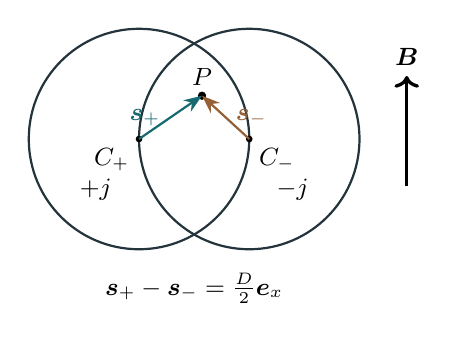
\begin{tikzpicture}[x=1cm,y=1cm]
\draw[object] (-.7,0) circle(1.4);\draw[object] (.7,0) circle(1.4);\coordinate (P) at (.1,.55);
\fill (-.7,0) circle(1.2pt) node[below left] {$C_+$};\fill (.7,0) circle(1.2pt) node[below right] {$C_-$};\fill (P) circle(1.5pt) node[above] {$P$};\draw[motion] (-.7,0)--(P) node[midway,left] {$\vect s_+$};\draw[force] (.7,0)--(P) node[midway,right] {$\vect s_-$};\draw[very thick,->] (2.7,-.6)--(2.7,.8) node[above] {$\vect B$};\node at (0,-1.9) {$\vect s_+-\vect s_-=\frac D2\vect e_x$};\node at (-1.25,-.65) {$+j$};\node at (1.25,-.65) {$-j$};
\end{tikzpicture}\figcaption{解图电2.5A　补成两个完整均匀圆柱，空隙中的虚构电流逐点相消。}\end{minipage}\end{center}

用两圆相交的几何关系求月牙截面积。令$r=D/2$，解图电2.5B的两轴间距为r。
连结$C_+$、$C_-$与上交点T，得到边长r的等边三角形；上、下交点对左圆心张角$2\pi/3$。
透镜由两个相同的圆弓形组成，故
\[
S_{\rm lens}=2\left[\frac12r^2\frac{2\pi}{3}
-\frac12r^2\sin\frac{2\pi}{3}\right]
=\left(\frac{2\pi}{3}-\frac{\sqrt3}{2}\right)r^2.
\]
\begin{center}\begin{minipage}{.97\linewidth}\centering
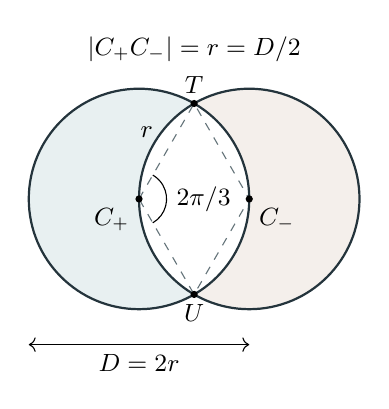
\begin{tikzpicture}[x=1cm,y=1cm,font=\small]
\fill[accent!10] (-.7,0) circle(1.4);
\fill[warm!10] (.7,0) circle(1.4);
\begin{scope}\clip (-.7,0) circle(1.4);\fill[white] (.7,0) circle(1.4);\end{scope}
\draw[object] (-.7,0) circle(1.4) (.7,0) circle(1.4);
\coordinate (L) at (-.7,0);\coordinate (R) at (.7,0);
\coordinate (T) at (0,1.2124);\coordinate (U) at (0,-1.2124);
\draw[guide] (L)--(T)--(R)--(U)--(L);
\fill (L) circle(1.3pt) node[below left] {$C_+$};
\fill (R) circle(1.3pt) node[below right] {$C_-$};
\fill (T) circle(1.3pt) node[above] {$T$};
\fill (U) circle(1.3pt) node[below] {$U$};
\draw (-.525,-.3031) arc(-60:60:.35);
\node at (.12,0) {$2\pi/3$};
\draw[<->] (-2.1,-1.85)--(.7,-1.85) node[midway,below] {$D=2r$};
\node[above left] at (-.4,.65) {$r$};
\node at (0,1.9) {$|C_+C_-|=r=D/2$};
\end{tikzpicture}
\figcaption{解图电2.5B　两圆半径为$r=D/2$、轴距也为r，透镜对应两个$2\pi/3$扇形减去两个三角形。左右月牙才是实际导体。}
\end{minipage}\end{center}

从一个完整圆中扣去透镜，解图电2.5B的一个月牙面积为
\[
A=\pi r^2-S_{\rm lens}
=\left(\frac\pi3+\frac{\sqrt3}{2}\right)r^2
=\left(\frac{\pi}{12}+\frac{\sqrt3}{8}\right)D^2.
\]
实际月牙内总电流为I，所以$j=I/A$。补全截面时沿用电流密度 $j$，因此完整圆柱的总电流增至 $I^\prime=j\pi r^2$。
两者关系也可从面积比先写出
\[
\frac{I}{I'}=\frac{A}{\pi D^2/4}
=\frac{2\pi+3\sqrt3}{6\pi}.
\]

完整圆柱的电流为
\[
 I'=j\frac{\pi D^2}{4}=\frac{6\pi I}{2\pi+3\sqrt3}.
\]
半径$D/2$的均匀轴向电流圆柱，在内部距自身轴线位矢$\vect s$处，由安培环路定律
\[
 B(2\pi s)=\mu_0 j\pi s^2,\qquad
 \vect B=\frac{\mu_0j}{2}\vect e_z\times\vect s.
\]
重叠区任意点同时位于两完整圆柱内部。相对两圆心的位矢为
\[
 \vect s_+=(x+D/4)\vect e_x+y\vect e_y,
 \quad\vect s_-=(x-D/4)\vect e_x+y\vect e_y.
\]
于是
\begin{align*}
 \vect B_+&=\frac{\mu_0j}{2}[-y\vect e_x+(x+D/4)\vect e_y],\\
 \vect B_-&=-\frac{\mu_0j}{2}[-y\vect e_x+(x-D/4)\vect e_y].
\end{align*}
\Needspace{10\baselineskip}

还可以在不展开坐标的情况下先看出消去原因：在解图电2.5A，同一点$P$的两个相对位矢满足
\[
\vect s_+-\vect s_-=\vect C_- -\vect C_+=\frac D2\vect e_x .
\]
因此$\vect B_++\vect B_-=(\mu_0j/2)\vect e_z\times(D\vect e_x/2)$，对空隙内任意$P$都相同。这里之所以两项均用内部场，是因为$P$同时落在两个完整圆柱内。

相加后含$x,y$的项全部消失：
\result{\vect B=\frac{\mu_0jD}{4}\vect e_y
 =\frac{6\mu_0 I}{(2\pi+3\sqrt3)D}\vect e_y.}
所以空隙中是匀强场。一般地，两相反均匀电流圆柱的共同内部区域，有$\vect B=(\mu_0j/2)\vect e_z\times(\vect C_--\vect C_+)$；均匀性来自内部场对位矢的线性关系。

解图电2.5C把同一点的两个分场画在一起。正向左柱在P给
$B_{+x}=-\mu_0jy/2$，负向右柱给$B_{-x}=+\mu_0jy/2$，水平分量逐点抵消。
两者的竖直分量之和为
\[
\frac{\mu_0j}{2}\left(x+\frac D4\right)
-\frac{\mu_0j}{2}\left(x-\frac D4\right)
=\frac{\mu_0jD}{4}.
\]
\begin{center}\begin{minipage}{.97\linewidth}\centering
\begin{tikzpicture}[x=1cm,y=1cm,font=\small]
\draw[guide] (-.7,0) circle(1.4) (.7,0) circle(1.4);
\coordinate (P) at (.1,.55);
\coordinate (A) at (-.45,1.35);
\coordinate (B) at (.65,1.15);
\coordinate (S) at (.1,1.95);
\fill (P) circle(1.4pt) node[below] {$P$};
\fill (-.7,0) circle(1.2pt) node[below left] {$C_+$};
\fill (.7,0) circle(1.2pt) node[below right] {$C_-$};
\draw[motion] (P)--(A) node[above left,fill=white,inner sep=1pt] {$\boldsymbol B_+$};
\draw[force] (P)--(B) node[right] {$\boldsymbol B_-$};
\draw[object,->] (P)--(S) node[above] {$\boldsymbol B\parallel+y$};
\draw[guide] (A)--(S)--(B);
\node at (0,-1.95) {两箭头水平分量相反，竖直分量相加};
\end{tikzpicture}
\figcaption{解图电2.5C　取与A图相同的P，各磁场按共同正比例缩放。两分场与合场同起点；P 点的两分场叠加给空隙中的合场。}
\end{minipage}\end{center}

移动P时，A图两条相对位矢都增加同一个位移，它们的差保持不变；
C图两个分场的坐标项因而继续约消，得到同一合场。空隙中 $\nabla\times\boldsymbol B=0$。这里还得到更强的结论：两个完整圆柱的内部场对相对位矢呈线性，因电流密度大小相等、方向相反，位置项逐点相消，留下常矢量。
离开两圆公共内部区后，至少一个圆柱要改用外部场公式，刚才的线性约消不再适用。

逐区读解图电2.5A：左月牙为 $+j$，右月牙为 $-j$，透镜内补入的两项相消，两圆外两项都是零。因此两完整柱的总电流分布处处等于实际月牙分布，磁场可由完整柱场相加。


\Needspace{18\baselineskip}

\pdfbookmark[2]{第 6 题 有限厚电流层的磁场分布}{q6}

\section*{第 6 题\quad 有限厚电流层的磁场分布}\label{q:6}

真空中$-d\le x\le d$的无限平面层沿$y,z$方向无限延伸，层内均匀电流密度为$\vect j=j\vect e_z$，其中$j>0$。无其他外加磁场。求全空间的磁感应强度分布。

\begin{center}\begin{minipage}{.98\linewidth}\centering
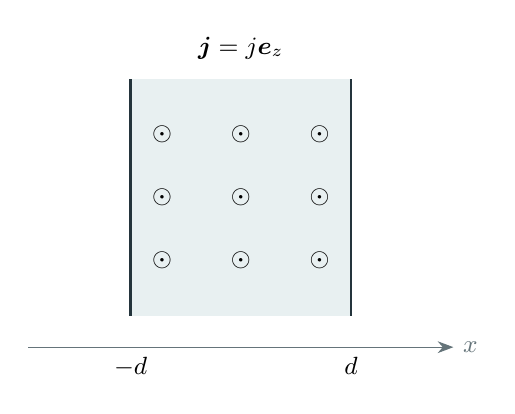
\begin{tikzpicture}[x=1cm,y=1cm]
\fill[accent!10] (-1.4,-1.5) rectangle(1.4,1.5);\draw[object] (-1.4,-1.5)--(-1.4,1.5);\draw[object] (1.4,-1.5)--(1.4,1.5);\foreach \x in {-1,0,1}\foreach \y in {-.8,0,.8}\node at (\x,\y) {$\odot$};\draw[axis] (-2.7,-1.9)--(2.7,-1.9) node[right] {$x$};\node[below] at (-1.4,-1.9) {$-d$};\node[below] at (1.4,-1.9) {$d$};\node at (0,1.9) {$\vect j=j\vect e_z$};
\end{tikzpicture}\figcaption{图电2.6　截面中圆点表示向外的电流；层沿y和z无限延伸。}\end{minipage}\end{center}

\Needspace{6\baselineskip}\subsection*{解答}

先确定场的方向，再求大小。将体电流分解成平行$z$轴的直线电流，每根线在场点的磁场都在$xy$平面内，故$B_z=0$。关于经过场点的$xz$平面对称的两根线，其$x$分量相消、$y$分量相加，因此只剩$B_y(x)$。解图电2.6A的高斯盒也能给出法向分量，并显示各面对净磁通的贡献。

电流分布在$y,z$方向具有平移对称性，所以本层产生的场只依赖$x$。将整个电流层绕$z$轴转过$180^\circ$，电流分布不变；
场的两个平面分量随之反向，再用y方向的平移不变性，得到
\[
B_x(-x)=-B_x(x),\qquad B_y(-x)=-B_y(x).
\]
以上奇性针对题设无外加磁场时电流层产生的场；叠加均匀场后，总场一般不再具有这一奇性。
\begin{center}\begin{minipage}{.97\linewidth}\centering
\begin{tikzpicture}[x=1cm,y=1cm,font=\small]
\draw[object] (-1.65,-.875)--(1.15,-.875)--(1.15,.525)--(-1.65,.525)--cycle;
\draw[guide] (-1.15,-.525)--(1.65,-.525)--(1.65,.875)--(-1.15,.875)--cycle;
\draw[object] (-1.65,-.875)--(-1.15,-.525) (1.15,-.875)--(1.65,-.525)
(1.15,.525)--(1.65,.875) (-1.65,.525)--(-1.15,.875);
\draw[force] (1.4,0)--(2.65,0) node[right] {$B_x(x_0)$};
\draw[force] (-1.4,0)--(-2.65,0) node[left] {$-B_x(x_0)$};
\draw[guide] (1.45,.6)--(2.2,1.2) node[right] {$\Delta S\ (yz\text{面})$};
\node[below] at (-1.4,-.9) {$-x_0$};
\node[below] at (1.4,-.9) {$x_0$};
\node at (0,1.65) {两$z$面通量为零，两$y$面通量相消};
\end{tikzpicture}
\figcaption{解图电2.6A　边沿$x,y,z$方向的闭合高斯盒。仅画法向场分量 $B_x$。两侧外法线和场分量均反向，故两通量同号，由无散定律得 $B_x=0$。}
\end{minipage}\end{center}

取解图电2.6A的盒子，x侧面在$\pm x_0$，每个$yz$侧面的面积为$\Delta S$。
将六面磁通按法线方向归类：
\[
0=\iint_{\partial V}\boldsymbol B\cdot\mathrm d\boldsymbol S
=\Phi_{xy}+\Phi_{xz}+\Phi_{yz}.
\]
两个$xy$面法线沿z，而$B_z=0$，所以$\Phi_{xy}=0$。
两个$xz$面法线沿$\pm y$，同一x处的$B_y(x)$不依赖y，通量成对相消，所以$\Phi_{xz}=0$；
若利用上面的奇性，也可直接看到各面上$\int_{-x_0}^{x_0}B_y(x)\,\mathrm dx=0$。
于是只剩两个$yz$面：
\[
\Phi_{yz}=[B_x(x_0)-B_x(-x_0)]\Delta S
=2B_x(x_0)\Delta S=0,\qquad B_x(x_0)=0.
\]
A图左、右两面的外法线和待定场分量同时反向，两个点积同号，和为一个面的两倍。无散定律要求它们都为零；任意$x_0$均成立，因而全空间只有$B_y(x)$。

\begin{center}\begin{minipage}{.97\linewidth}\centering
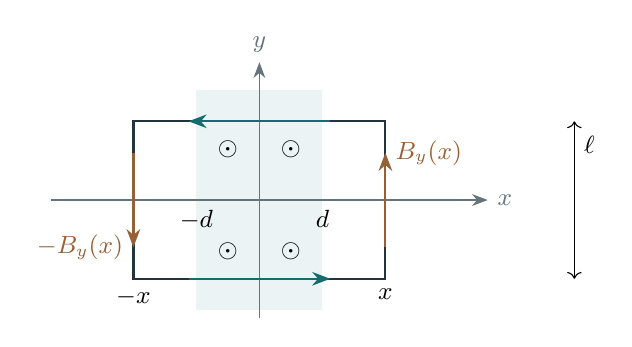
\begin{tikzpicture}[x=1cm,y=1cm,font=\small]
\fill[accent!8] (-.8,-1.4) rectangle(.8,1.4);
\draw[axis] (-2.65,0)--(2.9,0) node[right] {$x$};
\draw[axis] (0,-1.5)--(0,1.75) node[above] {$y$};
\draw[object] (-1.6,-1)--(1.6,-1)--(1.6,1)--(-1.6,1)--cycle;
\draw[motion] (-.9,-1)--(.9,-1);
\draw[motion] (.9,1)--(-.9,1);
\draw[force] (1.6,-.6)--(1.6,.6) node[right] {$B_y(x)$};
\draw[force] (-1.6,.6)--(-1.6,-.6) node[left] {$-B_y(x)$};
\draw[<->] (4,-1)--(4,1) node[pos=.85,right] {$\ell$};
\node[below] at (-1.6,-1) {$-x$};\node[below] at (1.6,-1) {$x$};
\node[below] at (-.8,0) {$-d$};\node[below] at (.8,0) {$d$};
\foreach \xx in {-.4,.4}\foreach \yy in {-.65,.65}\node at (\xx,\yy) {$\odot$};
\end{tikzpicture}
\figcaption{解图电2.6B　安培回路在$xy$平面，正向对应法线$+z$。两条竖边长度为$\ell$，水平间距为$2x$；图示$x>d$，载流宽度只到$2d$。}
\end{minipage}\end{center}


取解图电2.6B中关于$x=0$对称的矩形安培回路，其两长边平行$y$轴、长$\ell$，位于$\pm x$。按图选回路方向，$x>0$侧磁场沿正$y$轴，两长边环量相加。
当$0\le x\le d$时，包围电流为$j(2x\ell)$，故
\[
 2B_y(x)\ell=\mu_0 j(2x\ell),\qquad B_y(x)=\mu_0jx.
\]
当$x\ge d$时，包围电流不再随回路加宽而增加：
\[
 2B_y(x)\ell=\mu_0j(2d\ell),\qquad B_y(x)=\mu_0jd.
\]
利用奇对称性补齐负半空间，得
\result{\vect B(x)=\begin{cases}
 -\mu_0jd\vect e_y,&x<-d,\\
 \mu_0jx\vect e_y,&|x|\le d,\\
 \mu_0jd\vect e_y,&x>d.
 \end{cases}}

\begin{center}\begin{minipage}{.97\linewidth}\centering
\begin{tikzpicture}[x=1cm,y=1cm,font=\small]
\fill[accent!7] (-1.5,-1.45) rectangle(1.5,1.45);
\draw[axis] (-3.4,0)--(3.45,0) node[right] {$u=x/d$};
\draw[axis] (0,-1.65)--(0,1.8) node[above] {$B_y/(\mu_0jd)$};
\draw[traj] (-3,-1.2)--(-1.5,-1.2)--(1.5,1.2)--(3,1.2);
\draw[guide] (-1.5,0)--(-1.5,-1.2)--(0,-1.2) (1.5,0)--(1.5,1.2)--(0,1.2);
\node[below] at (-1.5,0) {$-1$};\node[below] at (1.5,0) {$1$};
\node[left] at (0,1.2) {$1$};\node[left] at (0,-1.2) {$-1$};
\node at (.7,-1.4) {载流层};
\end{tikzpicture}
\figcaption{解图电2.6C　归一化场曲线。对应的$B_y(x)$在层内斜率为$\mu_0j$，层外斜率为零；$x=\pm d$处场连续，斜率改变。阴影只标对应的载流横坐标区间。}
\end{minipage}\end{center}
在解图电2.6C的右侧层面，内侧极限$B_y(d^-)=\mu_0jd$与外侧极限$B_y(d^+)=\mu_0jd$相同；左侧同理。导数则从层内$\mu_0j$变成层外0。有限体电流密度的阶跃改变场的斜率；场在无额外面电流的层面连续通过。

也可把体电流分成薄片，按薄片在两侧的场分量相加。厚$\dd x'$的薄层等效面电流为$\dd K=j\dd x'$，在其右侧给$+\mu_0\dd K/2$的$y$分量，左侧给相反分量。对层内点$x$，
\[B_y(x)=\frac{\mu_0j}{2}\left[
\int_{-d}^{x}\dd x'-\int_x^d\dd x'\right]
=\mu_0jx.\]
对$x>d$，所有薄层都给同向贡献，得到$\mu_0j(2d)/2=\mu_0jd$。解图电2.6C中场的线性支与平台支由此都能解释，都由薄片累计的电流给出。

C图同时给出方向和大小：右半空间$B_y>0$，左半空间$B_y<0$；层内大小随$|x|$增加，层外大小恒定。若叠加均匀外场，对称回路只能求出两长边的场差；题设的无外场条件才确定这里的绝对场值。

\Needspace{18\baselineskip}

\pdfbookmark[2]{第 7 题 载流圆柱内的电子收缩与净电荷}{q7}

\section*{第 7 题\quad 载流圆柱内的电子收缩与净电荷}\label{q:7}

无限长圆柱导体未通电时，电子体电荷密度为$\rho_0<0$，固定正离子体电荷密度为$-\rho_0$。通电后电子以均匀轴向漂移速率$u<c$运动，磁力使电子趋向中轴，产生径向电场。假定电子在所占据的轴对称体区域内已达到电力与磁力平衡。求该区域的电子密度和净体电荷密度；说明有限截面导线中电荷守恒对边缘分布的限制。

\begin{center}\begin{minipage}{.97\linewidth}\centering
\begin{tikzpicture}[x=1cm,y=1cm,font=\small]
\fill[warm!8] (0,0) circle(1.7);
\fill[accent!10] (0,0) circle(1.36);
\draw[object] (0,0) circle(1.7);
\draw[guide] (0,0) circle(1.36);
\draw[axis] (0,0)--(2.6,0) node[right] {$r$};
\draw[<->] (0,0)--(135:1.36) node[pos=.75,below left] {$r_e$};
\draw[<->] (0,-2.05)--(1.7,-2.05) node[midway,below] {$R$};
\node at (.2,.6) {电子体区};
\node at (.15,-.55) {$\rho<0$};
\node at (0,2.2) {$\odot\,j_z>0,\qquad\otimes\,\boldsymbol u$};
\end{tikzpicture}
\figcaption{图电2.7　电子平均速度指向纸内（$-z$），常规电流指向纸外（$+z$）。外圆半径为$R$，虚圆示意待求的电子体区边界$r_e$。}
\end{minipage}\end{center}


\Needspace{6\baselineskip}\subsection*{解答}

取电子平均速度$\vect u=-u\vect e_z$，常规电流沿正$z$。解图电2.7A中电子受磁力径向向内，所需平衡电力向外，因此电场应向内，电子区域呈负的净体电荷。记电子密度$\rho(r)<0$，净密度$\Delta(r)=\rho(r)-\rho_0$。

\begin{center}\begin{minipage}{.97\linewidth}\centering
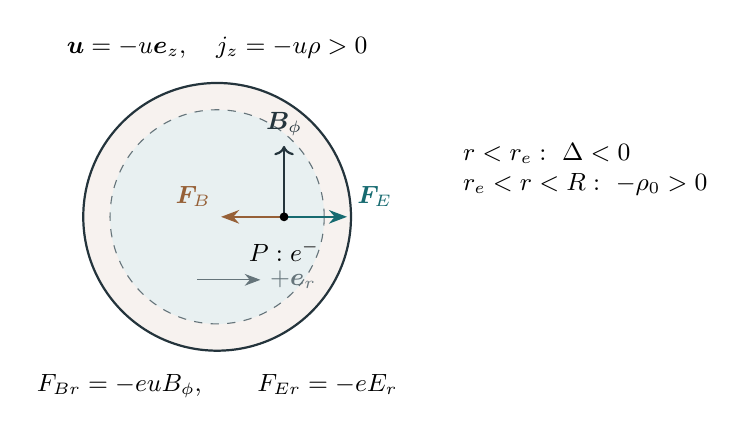
\begin{tikzpicture}[x=1cm,y=1cm,font=\small]
\fill[warm!8] (0,0) circle(1.7);
\fill[accent!10] (0,0) circle(1.36);
\draw[object] (0,0) circle(1.7);
\draw[guide] (0,0) circle(1.36);
\coordinate (P) at (.85,0);
\draw[force] (P)--(.05,0) node[above left] {$\boldsymbol F_B$};
\draw[motion] (P)--(1.65,0) node[above right] {$\boldsymbol F_E$};
\draw[object,->] (P)--(.85,.9) node[above] {$\boldsymbol B_\phi$};
\fill (P) circle(1.6pt) node[below=5pt] {$P:e^-$};
\draw[axis] (-.25,-.8)--(.55,-.8) node[right] {$+\boldsymbol e_r$};
\node at (0,2.15) {$\boldsymbol u=-u\boldsymbol e_z,\quad j_z=-u\rho>0$};
\node[right,align=left] at (3.0,.6) {$r<r_e:\ \Delta<0$\\$r_e<r<R:\ -\rho_0>0$};
\node at (0,-2.15) {$F_{Br}=-euB_\phi,\qquad F_{Er}=-eE_r$};
\end{tikzpicture}
\figcaption{解图电2.7A　右侧电子P的两力共起点、等大反向。局部磁场沿$+\boldsymbol e_\phi$，磁力向轴，电力离轴；电子带负电，所以电场向轴。}
\end{minipage}\end{center}
A图按径向向外取正，电子电荷为$-e$。在右侧P点，$\boldsymbol u\times\boldsymbol B=uB_\phi\boldsymbol e_r$，故
\[
F_{Br}=-euB_\phi<0,\qquad F_{Er}=-eE_r,\qquad
F_{Br}+F_{Er}=-e(uB_\phi+E_r)=0.
\]
取径向向外为正，得到 $E_r=-uB_\phi<0$。
\begin{center}\begin{minipage}{.97\linewidth}\centering
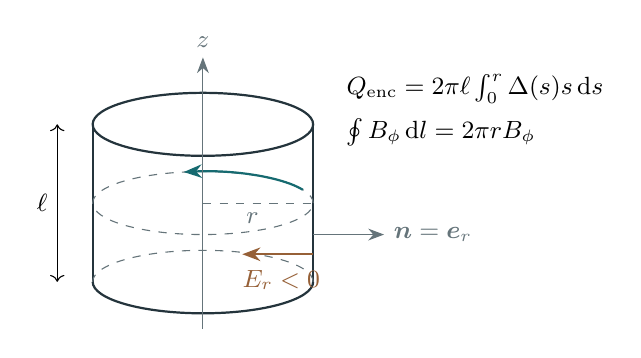
\begin{tikzpicture}[x=1cm,y=1cm,font=\small]
\draw[object] (-1.4,-1)--(-1.4,1) (1.4,-1)--(1.4,1);
\draw[object] (0,1) ellipse(1.4 and .4);
\draw[object] (-1.4,-1) arc(180:360:1.4 and .4);
\draw[guide] (1.4,-1) arc(0:180:1.4 and .4);
\draw[guide] (0,0) ellipse(1.4 and .4);
\draw[motion] (25:1.4 and .4) arc(25:100:1.4 and .4);
\draw[axis] (0,-1.6)--(0,1.85) node[above] {$z$};
\draw[guide] (0,0)--(1.4,0) node[pos=.45,below] {$r$};
\draw[force] (1.4,-.65)--(.5,-.65) node[pos=.45,below=2pt] {$E_r<0$};
\draw[axis] (1.4,-.4)--(2.3,-.4) node[right] {$\boldsymbol n=\boldsymbol e_r$};
\draw[<->] (-1.85,-1)--(-1.85,1) node[midway,left] {$\ell$};
\node[right] at (1.7,.9) {$\oint B_\phi\,\mathrm dl=2\pi rB_\phi$};
\node[right] at (1.7,1.45) {$Q_{\rm enc}=2\pi\ell\int_0^r\Delta(s)s\,\mathrm ds$};
\end{tikzpicture}
\figcaption{解图电2.7B　取在电子体区内的同轴高斯柱与圆形安培环路。高斯柱侧面外法线向外，电场向内，故通量为负；顶、底面通量为零。}
\end{minipage}\end{center}

在解图电2.7B中，半径为$r$的圆周上$B_\phi$恒定，安培定律为$2\pi rB_\phi=\mu_0I(r)$。
高斯柱侧面积为$2\pi r\ell$，端面法线沿z、电场沿径向，端面通量为零，因而
\[
2\pi r\ell E_r=\frac{Q_{\rm enc}}{\varepsilon_0}
=\frac{2\pi\ell}{\varepsilon_0}\int_0^r[\rho(s)-\rho_0]s\,\mathrm ds.
\]
约去公共因子后，分别得到下面两条场的积分式；安培式只计运动电子，高斯式计电子与固定离子的净电荷。


半径$r$的安培环路包围电流
\[
 I(r)=2\pi\int_0^r[-u\rho(s)]s\dd s,
 \quad B_\phi(r)=-\frac{\mu_0u}{r}\int_0^r\rho(s)s\dd s.
\]
同轴高斯柱给出
\[
 E_r(r)=\frac1{\varepsilon_0r}\int_0^r[\rho(s)-\rho_0]s\dd s.
\]
电子电荷为$-e$。其径向平衡要求$E_r=-uB_\phi$。代入上述两个积分式，设$\beta=u/c$、$c^{-2}=\varepsilon_0\mu_0$，整理得
\[
 (1-\beta^2)\int_0^r\rho(s)s\dd s=\frac{\rho_0r^2}{2}.
\]

\Needspace{9\baselineskip}
展开平衡式的消元过程为
\[
\int_0^r\rho(s)s\dd s-\frac{\rho_0r^2}{2}
=\varepsilon_0\mu_0u^2\int_0^r\rho(s)s\dd s .
\]
右端只积电子密度，因为固定离子不产生这股电流。把右端移到左边便得到$1-\beta^2$；A图电子体区由这个平衡式决定，外侧补偿区还须结合电子数守恒求出。

对$r$求导（$r>0$），再用轴上连续性补至$r=0$：
\result{\rho(r)=\frac{\rho_0}{1-\beta^2},\qquad
 \Delta(r)=\frac{\beta^2\rho_0}{1-\beta^2}<0.}
电子体区的结果确为常量；小速率下$\Delta\simeq\rho_0u^2/c^2$，变化极小。

体区密度由力平衡给出；其截面大小由每单位长度的电子数守恒决定。若通电前导线半径为$R$、每单位长度电子数守恒，采用理想锐边收缩模型，电子柱半径$r_e$还须满足
\[
 \rho\,\pi r_e^2=\rho_0\pi R^2,
 \qquad r_e=R\sqrt{1-\beta^2}.
\]
以单位长度计，解图电2.7A的两个区域分别携带净电荷
\[
\lambda_{\rm in}=\Delta\,\pi r_e^2
=\beta^2\rho_0\pi R^2,\qquad
\lambda_{\rm out}=-\rho_0\pi(R^2-r_e^2)
=-\beta^2\rho_0\pi R^2.
\]
两者之和为零，与A图内负、外正的分区相符。电子总数保持不变，增加的负密度由占据面积缩小来补偿；体区的电子电量用缩小后的面积计算。
在这个无限长、轴对称、总电中性的模型中，导线外的径向电场为零，
而总电流产生的外部磁场仍可非零。

外侧$r_e<r<R$为正离子补偿区，净密度$-\rho_0$；其正电量恰好抵消内区多出的负电量。以上分区采用电子柱外缘截断的模型。对给定的其他边缘分布，守恒式仍要求总电子线电荷等于通电前的值。

令 $A=-\rho_0>0$，分段求导线内外的场。锐边模型中，
$\rho=-A/(1-\beta^2)$在$r<r_e$内恒定，$r_e^2=(1-\beta^2)R^2$。
于是电子体区的带符号场为
\[
E_r=-\frac{A\beta^2r}{2\varepsilon_0(1-\beta^2)},\qquad
B_\phi=\frac{\mu_0uAr}{2(1-\beta^2)},\qquad 0\le r\le r_e.
\]
在$r_e<r<R$，高斯柱还包围部分正离子补偿环，总净线电荷为
$\lambda(r)=\lambda_{\rm in}+A\pi(r^2-r_e^2)=A\pi(r^2-R^2)$；
安培环路则已经包围全部电子电流$I=uA\pi R^2$。因此
\[
E_r=\frac{A}{2\varepsilon_0}\left(r-\frac{R^2}{r}\right),\qquad
B_\phi=\frac{\mu_0uAR^2}{2r},\qquad r_e<r<R.
\]
当$r\ge R$时，$E_r=0$，而$B_\phi=\mu_0I/(2\pi r)$。
代入$r=r_e$可见内区、补偿区两式的E和B分别相等；在$r=R$，
电场从负值连续回到零，磁场继续按$1/r$变化。这正是解图电2.7C的两条曲线。
\begin{center}\begin{minipage}{.97\linewidth}\centering
\begin{tikzpicture}[x=2.4cm,y=1.25cm,font=\small]
\fill[accent!7] (0,-.6) rectangle(.8,1.65);
\fill[warm!8] (.8,-.6) rectangle(1,1.65);
\draw[axis] (0,0)--(2.35,0) node[right] {$t=r/R$};
\draw[axis] (0,-.75)--(0,1.9) node[above] {$B_\phi/B_*,\quad E_r/E_*$};
\draw[traj,domain=0:.8,samples=40] plot(\x,{25*\x/16});
\draw[traj,domain=.8:2.15,samples=80] plot(\x,{1/\x});
\draw[thick,warm,domain=0:.8] plot(\x,{-9*\x/16});
\draw[thick,warm,domain=.8:1,samples=40] plot(\x,{\x-1/\x});
\draw[thick,warm] (1,0)--(2.15,0);
\draw[guide] (.8,-.6)--(.8,1.65) (1,-.6)--(1,1.65);
\node[above=5pt] at (.8,0) {$4/5$};
\node[below=5pt] at (1,0) {$1$};
\node[right,accent] at (2.15,.4651) {$B_\phi/B_*$};
\node[below,warm] at (1.7,-.18) {$E_r/E_*$};
\node at (.35,-.95) {电子体区};
\node[align=center] at (1.2,-1.15) {正补偿区\\$4/5<t<1$};
\end{tikzpicture}
\figcaption{解图电2.7C　守恒锐边模型的真实分段场，示意取$\beta=3/5$、$r_e/R=4/5$。其中$E_*=-\rho_0R/(2\varepsilon_0)>0$，$B_*=-\mu_0u\rho_0R/2>0$；实际漂移速率远小于此示意值。}
\end{minipage}\end{center}

C图在$r_e$处的磁场斜率改变，因为体电流到此截止；电场也因净体电荷改变而换支，
场值在分区交界连续；这个模型的电荷与电流都分布在有限体积内。


\Needspace{18\baselineskip}

\pdfbookmark[2]{第 8 题 磁场中转杆与滑动带电环}{q8}

\section*{第 8 题\quad 磁场中转杆与滑动带电环}\label{q:8}

光滑刚性细杆在水平面内绕固定竖直轴无摩擦旋转，杆对该轴的转动惯量为$J$。质量$m$、电荷$q>0$的小环套在杆上，与杆间无电荷转移。匀强磁场$B$垂直水平面向里，正转向取逆时针。
\begin{enumerate}
\item 小环在非零半径处相对杆静止时，求杆可能的非零角速度。
\item 杆初角速度$\omega_0>qB/m$，小环起初位于轴处，受微小扰动后沿杆外移。环能否在某个非零半径处径向停下，并从此相对杆保持静止？
\item 把初角速度变成$\alpha\omega_0$（$\alpha>0$），若要保持小环的空间轨道相同，磁场大小应怎样改变？
\end{enumerate}

\begin{center}\begin{minipage}{.98\linewidth}\centering
\begin{tikzpicture}[x=1cm,y=1cm]
\draw[object] (-.8,0)--(4,0);\fill (0,0) circle(2.5pt) node[below] {转轴};\draw[fill=white,thick] (2.2,0) circle(.13);\node[above] at (2.2,.18) {$m,q$};\draw[<->] (0,-.5)--(2.2,-.5) node[midway,below] {$r$};\draw[motion] (.8,.4) arc(25:115:.9) node[above] {$\omega$};\node at (3.6,1.1) {$\otimes B$};\node at (-.6,1.3) {$J$};
\end{tikzpicture}\figcaption{图电2.8　俯视转杆，角速度正向为逆时针。}\end{minipage}\end{center}

\Needspace{6\baselineskip}\subsection*{解答}

用$r$表示环到转轴的距离。图电2.8中正角速度给出逆时针切向速度，正电荷在向里磁场中受向轴的径向磁力；外移径向速度又产生正切向磁力。

\begin{center}\begin{minipage}{.97\linewidth}\centering
\begin{tikzpicture}[x=1cm,y=1cm,font=\small]
\begin{scope}
\coordinate (P) at (1.4,0);
\draw[motion] (P)--(2.4,0) node[right] {$\dot r\boldsymbol e_r$};
\draw[motion] (P)--(1.4,1.4) node[above] {$r\omega\boldsymbol e_\phi$};
\draw[object,->] (P)--(2.4,1.4) node[above right] {$\boldsymbol v$};
\draw[guide] (2.4,0)--(2.4,1.4)--(1.4,1.4);
\fill (P) circle(1.6pt) node[below] {$P$};
\node at (1.7,-.75) {速度分解};
\end{scope}
\begin{scope}[shift={(6,0)}]
\coordinate (P) at (1.4,0);
\draw[force] (P)--(0,0) node[left] {$-qBr\omega\boldsymbol e_r$};
\draw[force] (P)--(1.4,1) node[above] {$qB\dot r\boldsymbol e_\phi$};
\draw[object,->] (P)--(0,1) node[above left] {$\boldsymbol F_B$};
\draw[guide] (0,0)--(0,1)--(1.4,1);
\fill (P) circle(1.6pt) node[below] {$P:q>0$};
\node at (1,-.75) {磁力分解};
\end{scope}
\node at (4.5,2) {$\boldsymbol B=-B\boldsymbol e_z\quad\otimes$};
\end{tikzpicture}
\figcaption{解图电2.8A　以 $P$ 为起点分别分解速度和磁力。磁力与总速度垂直，切向磁力对固定轴有力矩。}
\end{minipage}\end{center}


\textbf{相对静止。} 解图电2.8A中径向磁力提供圆周运动所需合力。环随杆作圆周运动，径向方程为$qB\omega r=m\omega^2r$。在$r>0,\omega\ne0$下，
\result{\omega_c=qB/m.}
另有整体静止的$\omega=0$分支，它不属于所问的非零转速。

由A图两个速度分量，磁力的功率和力矩分别为
\[
\boldsymbol F_B\cdot\boldsymbol v
=(-qBr\omega)\dot r+(qB\dot r)(r\omega)=0,\qquad
\tau_{Bz}=r(qB\dot r).
\]
杆对环的切向约束力记为$N_\phi$，其对环的功率为$N_\phi r\omega$，
反作用力对杆的功率为$-N_\phi r\omega$，在杆环系统中相消；固定轴的支承力不做功。
磁力的总功率为零，但对转轴留下上述力矩。因而用机械能守恒与角动量定理分别确定两个积分。

在写轴上微扰的能量前，先说明初态。若扰动把环移至$r(0)=\epsilon>0$，
并给定$\dot r(0)=v_\epsilon$、$\omega(0)=\omega_0$，精确积分常量是
\[
2E_\epsilon=(J+m\epsilon^2)\omega_0^2+mv_\epsilon^2,\qquad
C_\epsilon=(J+m\epsilon^2)\omega_0-\frac12qB\epsilon^2.
\]
以后任意r处满足$2E_\epsilon=(J+mr^2)\omega^2+m\dot r^2$、
$(J+mr^2)\omega-\tfrac12qBr^2=C_\epsilon$。
下面按题设的微扰极限取$\epsilon,v_\epsilon\to0$，得到$2E=J\omega_0^2$、$C=J\omega_0$。
若精确取 $r=\dot r=0$，环始终沿轴静止；题设的外移取从微小偏移启动所得的极限轨道。

对磁力矩从轴上微扰极限积分，完整过程为
\[
\mathrm dL=qBr\dot r\,\mathrm dt=qBr\,\mathrm dr,\qquad
L-L_0=\int_0^r qBs\,\mathrm ds=\frac12qBr^2.
\]
这里$L=(J+mr^2)\omega$、$L_0=J\omega_0$。

\textbf{从轴处外移。} 无摩擦且磁力不做功，杆环系统机械能守恒。磁力对固定轴有力矩$qB r\dot r$，所以机械角动量本身不守恒，而有
\begin{align*}
 J\omega_0^2&=(J+mr^2)\omega^2+m\dot r^2,\\
 \frac{\dd}{\dd t}[(J+mr^2)\omega]&=qBr\dot r.
\end{align*}
积分第二式，得到
\[
 (J+mr^2)\omega=J\omega_0+\frac12qBr^2.
\]
微扰开始处$r\to0$，径向加速度的系数为$\omega_0(m\omega_0-qB)/m>0$，与题设外移相符。

假设到$r=R_*$时$\dot r=0$，能量和角动量两式化为
\[
 J\omega_0^2=(J+mR_*^2)\omega^2,\quad
 (J+mR_*^2)\omega=J\omega_0+\tfrac12qBR_*^2.
\]
具体消元可先由能量式写出
$R_*^2=J(\omega_0^2-\omega^2)/(m\omega^2)$、$J+mR_*^2=J\omega_0^2/\omega^2$。
代入力矩积分式，得到
\[
\frac{J\omega_0^2}{\omega}-J\omega_0
=\frac{qBJ(\omega_0^2-\omega^2)}{2m\omega^2}.
\]
两边乘$2m\omega^2/J$，再移项，才得到下面的二次式；
$\omega>0$由$(J+mr^2)\omega=J\omega_0+\tfrac12qBr^2$保证。

消去$R_*^2$，得
\[
 (2m\omega_0-qB)\omega^2-2m\omega_0^2\omega+qB\omega_0^2=0.
\]
该二次式还能写成
\[
(\omega-\omega_0)
[(2m\omega_0-qB)\omega-qB\omega_0]=0.
\]
若使用求根公式，判别式中的$\sqrt{(m\omega_0-qB)^2}$应取
$|m\omega_0-qB|=m\omega_0-qB$，最后一步用到了$\omega_0>\omega_c$。
将两根分别代回能量式的半径关系，区分轴上的零半径和外侧转向半径。

一根$\omega=\omega_0$对应$R_*=0$；另一根为
\[
 \omega_* =\frac{qB\omega_0}{2m\omega_0-qB}.
\]

还可把非平凡根代回角动量关系，得到实际外侧转向半径。记$\omega_c=qB/m$，则
\[
 R_*^2=\frac{J(\omega_0-\omega_*)}{m(\omega_*-\omega_c/2)}
 =\frac{4J\omega_0(\omega_0-\omega_c)}{m\omega_c^2}>0 .
\]
由解图电2.8A的径向磁力，任意时刻满足
\[
\ddot r=r\omega(\omega-\omega_c).
\]
由于$\omega_0>\omega_c$，转向处有$0<\omega_*<\omega_c$，故$\ddot r_*<0$。小环在这里开始向内返回，径向速度从零转为负。

要从此停留还须$\omega_*=\omega_c$，这会推出$\omega_0=qB/m$，与严格不等式矛盾。题给初转速严格大于 $\omega_c$，所以外侧落在返回分支。持续共转的径向平衡与瞬时转向分别由 $\ddot r=0$ 与 $\dot r=0$ 描述。

外移段的径向速度可直接由能量式求出。把角速度积分式代入能量式，整理成
\[
\dot r^2=
\frac{r^2[J\omega_0(\omega_0-\omega_c)-m\omega_c^2r^2/4]}{J+mr^2}.
\]
当$0<r<R_*$时右端为正，外移分支取正平方根；到$R_*$时降为零。
该处是简单零点，到达外侧转向点的剩余时间积分收敛。杆长足以容纳 $R_*$ 时可到达转向点；若杆端在内侧，沿杆约束的解描述到杆端为止。
相反，近轴$\dot r\sim r\sqrt{\omega_0(\omega_0-\omega_c)}$，
在这一极限轨道上回到精确轴心需无限时间。有限$\epsilon$的运动须使用前面的精确常量。
\begin{center}\begin{minipage}{.97\linewidth}\centering
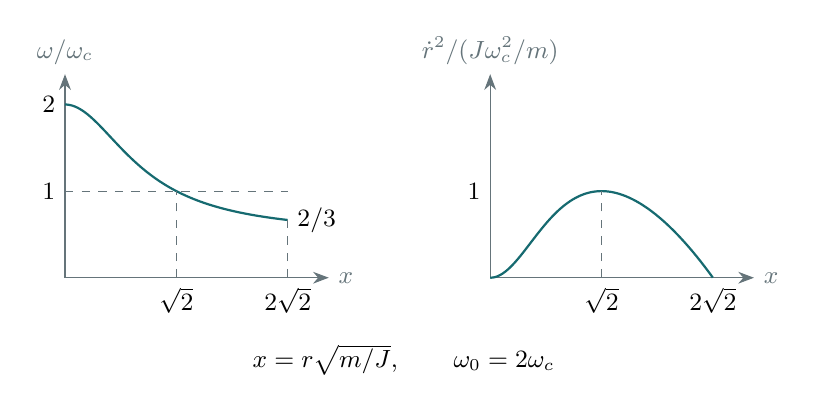
\begin{tikzpicture}[x=1cm,y=1.1cm,font=\small]
\begin{scope}
\draw[axis] (0,0)--(3.35,0) node[right] {$x$};
\draw[axis] (0,0)--(0,2.35) node[above] {$\omega/\omega_c$};
\draw[traj,domain=0:2.828427,samples=90] plot(\x,{(2+\x^2/2)/(1+\x^2)});
\draw[guide] (0,1)--(2.828427,1);
\draw[guide] (1.414214,0)--(1.414214,1) (2.828427,0)--(2.828427,.666667);
\node[left] at (0,2) {$2$};
\node[left] at (0,1) {$1$};
\node[below] at (1.414214,0) {$\sqrt2$};
\node[below] at (2.828427,0) {$2\sqrt2$};
\node[right] at (2.828427,.666667) {$2/3$};
\end{scope}
\begin{scope}[shift={(5.4,0)}]
\draw[axis] (0,0)--(3.35,0) node[right] {$x$};
\draw[axis] (0,0)--(0,2.35) node[above] {$\dot r^2/(J\omega_c^2/m)$};
\draw[traj,domain=0:2.828427,samples=90] plot(\x,{\x^2*(2-\x^2/4)/(1+\x^2)});
\draw[guide] (1.414214,0)--(1.414214,1);
\node[below] at (1.414214,0) {$\sqrt2$};
\node[below] at (2.828427,0) {$2\sqrt2$};
\node[left] at (0,1) {$1$};
\end{scope}
\node at (4.3,-.95) {$x=r\sqrt{m/J},\qquad\omega_0=2\omega_c$};
\end{tikzpicture}
\figcaption{解图电2.8B　微扰极限下的真实函数。角速度从$2\omega_c$降至外侧转向点的$2\omega_c/3$；径向速度平方先增后减，在$x=2\sqrt2$归零，此时角速度仍不满足共转平衡。}
\end{minipage}\end{center}

在解图电2.8B左侧曲线上，$\omega=\omega_c$时径向加速度瞬时为零，
对应$x=\sqrt2$；右图此处径向速率反而最大。到$x=2\sqrt2$时径向速率为零，
但$\omega=2\omega_c/3$，径向加速度向内。图上先经过径向加速度零点，再经过径向速度零点。

\textbf{轨道缩放。} 极坐标轨道由$\dd r/\dd\theta=\dot r/\omega$决定。联立守恒式可写为
\[
 \left(\frac{\dd r}{\dd\theta}\right)^2
 =\frac{J+mr^2}{m}\left[
 \frac{J(J+mr^2)}{(J+qBr^2/(2\omega_0))^2}-1\right].
\]
轨道导数的中间代数为
\[
m\left(\frac{\dot r}{\omega}\right)^2
=J\frac{\omega_0^2}{\omega^2}-(J+mr^2),\qquad
\omega=\frac{J\omega_0+\tfrac12qBr^2}{J+mr^2}.
\]
外移取$\mathrm dr/\mathrm d\theta>0$，内返取负支；比较轨道时也要选择对应的分支和相同初始方位。


初始位置、方位及运动分支相同，右端仅通过$B/\omega_0$依赖磁场和初角速度。故取
\result{B_{\rm new}=\alpha B}
即可保留同一空间轨道，运动时间相应缩为原来的$1/\alpha$。在精确轴上且无扰动的理想初态，$r=0$本身仍是解；这里讨论微扰触发的外移轨道。

从时间缩放也可直接看出同一轨道。把运动写为$r(t),\theta(t)$，令
$r_{\rm new}(t)=r(\alpha t)$、$\theta_{\rm new}(t)=\theta(\alpha t)$。
于是$\dot r_{\rm new}=\alpha\dot r$、$\omega_{\rm new}=\alpha\omega$，
$\ddot r_{\rm new}=\alpha^2\ddot r$；取$B_{\rm new}=\alpha B$后，
径向方程两端均乘$\alpha^2$，力矩方程两端也同乘$\alpha^2$，
所以这是同一轨道的时间重参数化。有限扰动时还须把初始径向速度同时乘$\alpha$；
若$v_\epsilon=0$，这一条件自动满足。解图电2.8C以实际积分的外移段标出同一点的两种历时。
\begin{center}\begin{minipage}{.97\linewidth}\centering
\begin{tikzpicture}[x=1cm,y=1cm,font=\small]
\draw[axis] (-1.6,0)--(2.7,0) node[right] {$X$};
\draw[axis] (0,-3)--(0,1) node[above] {$Y$};
\draw[traj] plot coordinates {(0.200000,0.000000) (0.199839,0.011329) (0.199356,0.022676) (0.198545,0.034056) (0.197398,0.045486) (0.195902,0.056981) (0.194042,0.068554) (0.191801,0.080218) (0.189157,0.091982) (0.186086,0.103855) (0.182561,0.115842) (0.178553,0.127945) (0.174031,0.140165) (0.168962,0.152496) (0.163311,0.164931) (0.157041,0.177459) (0.150117,0.190066) (0.142499,0.202730) (0.134151,0.215430) (0.125034,0.228137) (0.115111,0.240819) (0.104346,0.253438) (0.092705,0.265955) (0.080155,0.278323) (0.066665,0.290493) (0.052208,0.302410) (0.036759,0.314018) (0.020297,0.325254) (0.002807,0.336054) (-0.015724,0.346350) (-0.035304,0.356072) (-0.055933,0.365146) (-0.077609,0.373499) (-0.100322,0.381055) (-0.124057,0.387737) (-0.148791,0.393469) (-0.174497,0.398175) (-0.201140,0.401781) (-0.228680,0.404213) (-0.257071,0.405401) (-0.286259,0.405278) (-0.316186,0.403779) (-0.346789,0.400845) (-0.377998,0.396422) (-0.409740,0.390459) (-0.441937,0.382912) (-0.474509,0.373743) (-0.507370,0.362920) (-0.540435,0.350418) (-0.573615,0.336217) (-0.606821,0.320306) (-0.639962,0.302678) (-0.672948,0.283334) (-0.705690,0.262281) (-0.738100,0.239533) (-0.770089,0.215109) (-0.801575,0.189032) (-0.832473,0.161334) (-0.862704,0.132049) (-0.892192,0.101214) (-0.920863,0.068875) (-0.948647,0.035077) (-0.975477,-0.000131) (-1.001292,-0.036694) (-1.026031,-0.074559) (-1.049639,-0.113668) (-1.072066,-0.153963) (-1.093263,-0.195383) (-1.113186,-0.237868) (-1.131794,-0.281354) (-1.149050,-0.325779) (-1.164921,-0.371080) (-1.179375,-0.417194) (-1.192385,-0.464057) (-1.203927,-0.511606) (-1.213979,-0.559777) (-1.222522,-0.608510) (-1.229540,-0.657740) (-1.235019,-0.707406) (-1.238948,-0.757447) (-1.241317,-0.807803) (-1.242121,-0.858413) (-1.241353,-0.909219) (-1.239013,-0.960162) (-1.235098,-1.011185) (-1.229611,-1.062230) (-1.222554,-1.113242) (-1.213931,-1.164166) (-1.203751,-1.214948) (-1.192019,-1.265533) (-1.178747,-1.315870) (-1.163945,-1.365906) (-1.147625,-1.415592) (-1.129803,-1.464877) (-1.110493,-1.513712) (-1.089712,-1.562049) (-1.067477,-1.609841) (-1.043810,-1.657042) (-1.018729,-1.703606) (-0.992258,-1.749490) (-0.964418,-1.794649) (-0.935234,-1.839042) (-0.904731,-1.882628) (-0.872935,-1.925365) (-0.839874,-1.967214) (-0.805576,-2.008137) (-0.770071,-2.048097) (-0.733388,-2.087057) (-0.695559,-2.124983) (-0.656617,-2.161839) (-0.616593,-2.197594) (-0.575522,-2.232214) (-0.533439,-2.265669) (-0.490379,-2.297930) (-0.446379,-2.328968) (-0.401474,-2.358755) (-0.355704,-2.387265) (-0.309105,-2.414473) (-0.261718,-2.440355) (-0.213581,-2.464889) (-0.164735,-2.488052) (-0.115221,-2.509824) (-0.065078,-2.530187) (-0.014350,-2.549123) (0.036922,-2.566614) (0.088696,-2.582646) (0.140928,-2.597204) (0.193577,-2.610276) (0.246597,-2.621851) (0.299945,-2.631917) (0.353578,-2.640465) (0.407452,-2.647490) (0.461521,-2.652982) (0.515742,-2.656939) (0.570071,-2.659355) (0.624461,-2.660228) (0.678870,-2.659558) (0.733252,-2.657343) (0.787562,-2.653586) (0.841757,-2.648288) (0.895792,-2.641455) (0.949623,-2.633090) (1.003206,-2.623201) (1.056497,-2.611795) (1.109452,-2.598881) (1.162028,-2.584469) (1.214183,-2.568571) (1.265874,-2.551199) (1.317058,-2.532368) (1.367695,-2.512092) (1.417742,-2.490387) (1.467159,-2.467272) (1.515907,-2.442764) (1.563944,-2.416883) (1.611232,-2.389651) (1.657733,-2.361089) (1.703409,-2.331221) (1.748222,-2.300070) (1.792137,-2.267661) (1.835118,-2.234022) (1.877129,-2.199179)};
\fill (0,0) circle(1.5pt) node[above left] {$O$};
\fill (.2,0) circle(1.5pt) node[above right] {$P_0$};
\fill (-0.772020,-2.045962) circle(1.6pt) node[left] {$P$};
\draw[guide] (0,0)--(1.877129,-2.199179);
\fill (1.877129,-2.199179) circle(1.6pt) node[right] {$T$};
\node[right,align=left] at (3.1,-.3) {$\alpha=2$\\同一点P：\\旧历时$3$\\新历时$3/2$\\同一转向点T};
\end{tikzpicture}
\figcaption{解图电2.8C　有限微扰的实际共同外移轨迹，至首次外侧转向点T。采用无量纲$J=m=\omega_c=1$、$r(0)=1/5$、$\dot r(0)=0$、$\omega(0)=2$；按径向与角向方程积分。初角速度与磁场同时加倍后，每个位置的通过历时减半。}
\end{minipage}\end{center}


\Needspace{18\baselineskip}

\pdfbookmark[2]{第 9 题 地磁场中带电圆环的滑动与纯滚动}{q9}

\section*{第 9 题\quad 地磁场中带电圆环的滑动与纯滚动}\label{q:9}

半径$R$、质量$m$的均匀细圆环带有相对环固定的均匀正电荷$Q$，竖立在水平地面上。初态仅有向东的平动速度$v_0>0$，没有转动。地面动摩擦因数为$\mu>0$，均匀磁场$B$沿水平方向向北。忽略电磁辐射和形变。
\begin{enumerate}
\item 求圆环始终不离开地面的$v_0$范围。
\item 在达到纯滚动之前，求平动速度$v(t)$。
\item 当$v_0=mg/(2QB)$时，求达到纯滚动的时刻。
\end{enumerate}

\begin{center}\begin{minipage}{.98\linewidth}\centering
\begin{tikzpicture}[x=1cm,y=1cm]
\draw[object] (0,1.4) circle(1.4);\draw[object] (-2,0)--(3.6,0);\fill[pattern=north east lines] (-2,-.18) rectangle(3.6,0);\draw[motion] (1.7,1.4)--(3,1.4) node[right] {$v_0$};\node at (0,1.4) {$m,Q$};\node at (-1.8,2.7) {$\otimes B$};\node at (3,-.45) {$\mu$};\node at (-.8,-.45) {西};\node at (2.2,-.45) {东};
\end{tikzpicture}\figcaption{图电2.9　环竖直放置，初始向东平动，无初始自转。}\end{minipage}\end{center}

\Needspace{6\baselineskip}\subsection*{解答}

取向东为$x$正向、向上为$y$正向，北向磁场垂直图面向里。平动造成总磁力$QBv$向上；旋转造成各电荷的磁力相对圆心径向分布。

\begin{center}\begin{minipage}{.97\linewidth}\centering
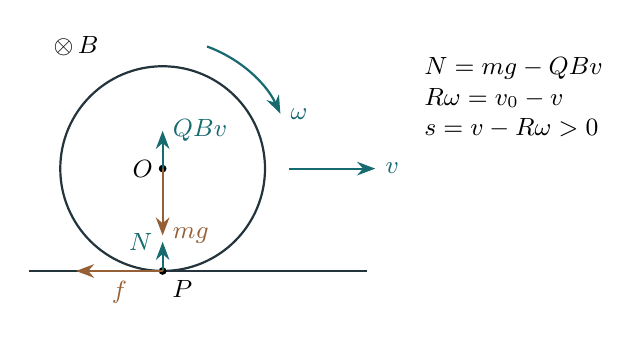
\begin{tikzpicture}[x=1cm,y=1cm,font=\small]
\draw[object] (0,1.3) circle(1.3);
\draw[object] (-1.7,0)--(2.6,0);
\fill (0,1.3) circle(1.4pt) node[left] {$O$};
\fill (0,0) circle(1.4pt) node[below right] {$P$};
\draw[force] (0,1.3)--(0,.45) node[right] {$mg$};
\draw[motion] (0,1.3)--(0,1.78) node[right] {$QBv$};
\draw[motion] (0,0)--(0,.37) node[left] {$N$};
\draw[force] (0,0)--(-1.1,0) node[midway,below] {$f$};
\draw[motion] (1.6,1.3)--(2.7,1.3) node[right] {$v$};
\draw[motion] (70:1.65) ++(0,1.3) arc(70:25:1.65) node[right] {$\omega$};
\node[align=left,right] at (3.2,2.2) {$N=mg-QBv$\\$R\omega=v_0-v$\\$s=v-R\omega>0$};
\node at (-1.1,2.85) {$\otimes\,B$};
\end{tikzpicture}
\figcaption{解图电2.9A　O为圆心，P为接触点。竖直合力为零；向西摩擦既使质心减速，又使环顺时针加速。纯滚动之前P向东滑，纯滚动后静摩擦取零即可维持匀速。}
\end{minipage}\end{center}


对任意电荷元$\dd Q$，速度是$\vect v+\vect\omega\times\vect r$。旋转项合力为
\[
 \int\dd Q\,[(\vect\omega\times\vect r)\times\vect B]=0,
\]
因为均匀环满足$\int\vect r\dd Q=0$，且磁场均匀。平动磁力对圆心的总力矩也为零；旋转磁力逐元径向，力矩同样为零。

按解图电2.9B写出旋转部分的径向力，取圆心相对位矢$\boldsymbol r=(x,y,0)$，顺时针角速度矢量为$-\omega\boldsymbol e_z$。于是
\[
\boldsymbol v_{\rm rot}=\omega y\boldsymbol e_x-\omega x\boldsymbol e_y,\qquad
\mathrm d\boldsymbol F_{\rm rot}
=\mathrm dQ\,\boldsymbol v_{\rm rot}\times(-B\boldsymbol e_z)
=\mathrm dQ\,\omega B\boldsymbol r.
\]
对正电荷元，该力沿半径向外。P与P$'$的位矢相反，所以两力反向抵消；力沿其位矢，逐元力矩也为零。
\begin{center}\begin{minipage}{.97\linewidth}\centering
\begin{tikzpicture}[x=1cm,y=1cm,font=\small]
\begin{scope}
\draw[object] (0,0) circle(1.1);
\draw[guide] (-.777817,-.777817)--(.777817,.777817);
\fill (.777817,.777817) circle(1.4pt) node[above left] {$P$};
\fill (-.777817,-.777817) circle(1.4pt) node[below right] {$P'$};
\draw[motion] (.777817,.777817)--(1.25,1.25) node[above right] {$\mathrm d\boldsymbol F_{\rm rot}$};
\draw[motion] (-.777817,-.777817)--(-1.25,-1.25);
\fill (0,0) circle(1pt) node[below right] {$O$};
\node at (0,-1.85) {旋转项：成对反向、逐元无矩};
\end{scope}
\begin{scope}[shift={(5.7,0)}]
\draw[object] (0,0) circle(1.1);
\fill (.777817,.777817) circle(1.4pt) node[below right] {$P$};
\fill (-.777817,-.777817) circle(1.4pt) node[below left] {$P'$};
\draw[force] (.777817,.777817)--(.777817,1.5) node[above] {$\mathrm dQ\,vB$};
\draw[force] (-.777817,-.777817)--(-.777817,-.055);
\draw[guide] (-.777817,0)--(.777817,0);
\fill (0,0) circle(1pt) node[below right] {$O$};
\node at (0,-1.85) {平动项：同向相加、成对消矩};
\end{scope}
\node at (2.7,2) {$\boldsymbol\omega=-\omega\boldsymbol e_z,\quad\boldsymbol B=-B\boldsymbol e_z$};
\end{tikzpicture}
\figcaption{解图电2.9B　P与P$'$携带相同电荷元。左图旋转磁力沿半径向外，成对合力为零，每个电荷元的力矩也为零；右图平动磁力都向上，其合力非零，而对圆心的力矩成对抵消。}
\end{minipage}\end{center}

平动项对圆心的力矩可直接写成
\[
\boldsymbol\tau_{\rm tr}
=\left(\int\boldsymbol r\,\mathrm dQ\right)\times(\boldsymbol v\times\boldsymbol B)=0,
\qquad
\boldsymbol\tau_{\rm rot}
=\int\boldsymbol r\times(\omega B\boldsymbol r)\,\mathrm dQ=0.
\]
解图电2.9A中的$QBv$因而代表整体合力，摩擦是唯一改变绕心机械角动量的外力。
均匀固定的电荷使电荷中心与圆心重合；均匀磁场使每一平动磁力只相差电荷元的权重，因此平动总力通过圆心。

\textbf{接触条件。} 支持力$N=mg-QBv$。初始接触要求$v_0\le v_g$，其中$v_g=mg/(QB)$。若$v_0<v_g$，摩擦使$v$下降，$N$随之增加，后来不会离地。等号时$N=0$、摩擦为零，圆环保持平动，始终不离地却不会转入纯滚动。故
\result{0<v_0\le\frac{mg}{QB}.}
\textbf{滑动阶段。} 对严格小于上界的情况，接触点向东滑动，摩擦向西，$f=\mu(mg-QBv)$。平动方程
\[
 m\dot v=-\mu(mg-QBv),\quad
 \frac{\dd(v_g-v)}{v_g-v}=\frac{\mu QB}{m}\dd t.
\]
从初速度积到当前速度，得到
\[
\int_{v_0}^{v(t)}\frac{\mathrm dv}{v_g-v}
=-\frac{\mu QB}{m}\int_0^t\mathrm dt,\qquad
\ln\frac{v_g-v(t)}{v_g-v_0}=\frac{\mu QB}{m}t.
\]
因$v_0<v_g$，分子、分母均为正。$v_g-v$随时间增加，该差以正指数增大，所以 $v$ 下降；在同一滑动支上，$N=QB(v_g-v)$和$f=\mu N$也随之增加。

利用$v(0)=v_0$，得
\result{v(t)=v_g-(v_g-v_0)\exp\left(\frac{\mu QB}{m}t\right),\quad0\le t\le T_r.}
到 $T_r$ 时换用纯滚动条件。

\textbf{转入纯滚动。} 令顺时针角速度大小为$\omega$，环的转动惯量$mR^2$，则
\[
 mR^2\dot\omega=fR,\qquad m\dot v=-f.
\]
消掉摩擦的积分可展开为
\[
\frac{\mathrm d\omega}{\mathrm dt}=-\frac1R\frac{\mathrm dv}{\mathrm dt},
\qquad
\int_0^\omega\mathrm d\omega=-\frac1R\int_{v_0}^v\mathrm dv.
\]
从A图接触点P的速度看，质心平动给向东的v，顺时针转动给向西的$R\omega$。
两种速度等大反向时，接触点相对地面静止，质心仍向东。

积分得$R\omega=v_0-v$；与纯滚动条件$R\omega=v$联立，有$v(T_r)=v_0/2$。所以
\[
 T_r=\frac m{\mu QB}\ln\frac{v_g-v_0/2}{v_g-v_0}.
\]

在纯滚动前，接触点相对地面的速度为
\[
v-R\omega=2v-v_0 .
\]
它从$v_0$连续降到0，在$0\le t<T_r$内始终向东，因而解图电2.9A中向西的动摩擦方向在整个积分阶段自洽。滑速到零后进入纯滚动段，以静摩擦关系描述接触。

将$v(T_r)=v_0/2$代入速度解，逐步得到
\[
e^{\mu QBT_r/m}=\frac{v_g-v_0/2}{v_g-v_0}.
\]
特别取$v_0=v_g/2$，右边为$(3v_g/4)/(v_g/2)=3/2$；
故解图电2.9C三条曲线在同一终止时刻满足$v=R\omega=v_g/4$、$s=0$。
\begin{center}\begin{minipage}{.97\linewidth}\centering
\begin{tikzpicture}[x=8cm,y=3.4cm,font=\small]
\draw[axis] (0,0)--(.51,0) node[right] {$\tau=\mu QBt/m$};
\draw[axis] (0,0)--(0,.7) node[above] {归一化速度};
\draw[traj,domain=0:.405465108,samples=80] plot(\x,{1-exp(\x)/2});
\draw[thick,warm,domain=0:.405465108,samples=80] plot(\x,{(exp(\x)-1)/2});
\draw[guide,domain=0:.405465108,samples=80] plot(\x,{1.5-exp(\x)});
\draw[guide] (.405465108,0)--(.405465108,.25)--(0,.25);
\node[left] at (0,.5) {$1/2$};
\node[left] at (0,.25) {$1/4$};
\node[below] at (.405465108,0) {$\ln(3/2)$};
\draw[traj] (.53,.59)--(.6,.59);
\node[right] at (.6,.59) {$v/v_g$};
\draw[thick,warm] (.53,.44)--(.6,.44);
\node[right] at (.6,.44) {$R\omega/v_g$};
\draw[guide] (.53,.29)--(.6,.29);
\node[right] at (.6,.29) {$s/v_g$};
\end{tikzpicture}
\figcaption{解图电2.9C　取$v_0=v_g/2$的实际速度曲线，$s=v-R\omega$。质心速度下降、转动线速度上升，在$\tau=\ln(3/2)$相等；接触点滑速恰在同一时刻归零，此后改用纯滚动方程。}
\end{minipage}\end{center}

用解图电2.9C的滑速还可求滑动耗散。磁力对每个电荷元的瞬时功率均为零，
而摩擦对质心平动的功率为$-fv$，对绕心转动的功率为$+fR\omega$；
前者使平动动能降低，后者使转动动能增加；两功率相加才得到整环机械能变化。系统动能及其变化率为
\[
K=\frac12mv^2+\frac12mR^2\omega^2
=\frac m2[v^2+(v_0-v)^2],\qquad
\frac{\mathrm dK}{\mathrm dt}
=m(2v-v_0)\dot v=-f(v-R\omega)=-fs\le0.
\]
在$T_r$时，两项动能各为$mv_0^2/8$，总动能为$mv_0^2/4$，
与初始$mv_0^2/2$相比，耗散$mv_0^2/4$。这部分机械能转化为接触处的热量。

B图旋转磁力虽逐元向外，但刚性圆环的内部约束承担这一径向作用；
题设忽略形变，所以R和$mR^2$保持不变。均匀质量与均匀固定电荷使质心、电荷中心和圆心重合，
各对径元才可按B图配对。这里的绕心力矩与惯量均按题给固定电荷和刚性细环计算。

到达纯滚动后，取$f_{\rm static}=0$就同时满足水平平动、绕心转动方程，
所以$v=v_0/2$、$\omega=v_0/(2R)$保持不变，$N=mg-QBv_0/2>0$。
这里的支持力在纯滚动阶段保持正值。

在$v_0=v_g/2$时，
\result{T_r=\frac m{\mu QB}\ln\frac32.}
若$B\to0$，一般式趋于$v_0/(2\mu g)$，与普通细圆环的滑动转滚动相符。

\Needspace{18\baselineskip}

\pdfbookmark[2]{第 10 题 电子枪击靶的圆轨道与螺旋轨道}{q10}

\section*{第 10 题\quad 电子枪击靶的圆轨道与螺旋轨道}\label{q:10}

电子经$U=1000\,\mathrm V$的电压从静止加速后，从枪口$T$沿直线$a$方向射出。靶$M$到$T$的距离$d=5.0\,\mathrm{cm}$，$TM$与初速度方向夹角$\phi=60^\circ$。求下列两种磁场下能击中$M$所需的磁感应强度：
\begin{enumerate}\item 磁场垂直于$a$和$TM$所在平面；选取使电子向靶偏转的方向。
\item 磁场平行$TM$，方向由$T$指向$M$。\end{enumerate}
电子质量$m_e=9.11\times10^{-31}\,\mathrm{kg}$，电荷绝对值$e=1.60\times10^{-19}\,\mathrm C$，采用非相对论近似。

\begin{center}\begin{minipage}{.98\linewidth}\centering
\begin{tikzpicture}[x=1cm,y=1cm]
\coordinate (T) at (0,1);\coordinate (M) at (1.5,-1.598);\draw[object] (-1.2,.85)--(0,.85)--(0,1.15)--(-1.2,1.15);\draw[motion] (T)--(2,1) node[right] {$v$};\draw[guide] (T)--(M) node[midway,below left] {$d$};\fill (M) circle(2pt) node[right] {$M$};\node[above] at (T) {$T$};\draw (.6,1) arc(0:-60:.6);\node at (.9,.72) {$\phi$};\node[right] at (3,1) {$a$};
\end{tikzpicture}\figcaption{图电2.10　目标方向与枪口初速度夹角为$\phi$。}\end{minipage}\end{center}

\Needspace{6\baselineskip}\subsection*{解答}

加速后$\tfrac12m_ev^2=eU$，故$v=\sqrt{2eU/m_e}=1.87\times10^7\,\mathrm{m/s}$。先由几何确定所需回转半径，再由动力学求场强。

\begin{center}\begin{minipage}{.97\linewidth}\centering
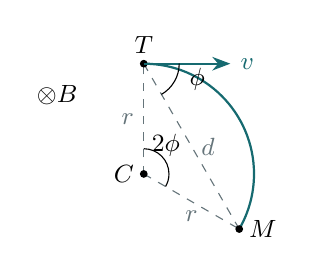
\begin{tikzpicture}[x=1cm,y=1cm,font=\small]
\coordinate (C) at (0,.2);
\coordinate (T) at ($(C)+(90:1.4)$);
\coordinate (M) at ($(C)+(-30:1.4)$);
\draw[traj] (T) arc(90:-30:1.4);
\draw[guide] (T)--(M) node[midway,right] {$d$};
\draw[guide] (C)--(T) node[midway,left] {$r$};
\draw[guide] (C)--(M) node[midway,below] {$r$};
\fill (T) circle(1.4pt) node[above] {$T$};
\fill (M) circle(1.4pt) node[right] {$M$};
\fill (C) circle(1.4pt) node[left] {$C$};
\draw[motion] (T)--($(T)+(1.1,0)$) node[right] {$v$};
\draw ($(T)+(.45,0)$) arc(0:-60:.45);
\node at (.68,1.4) {$\phi$};
\draw ($(C)+(90:.32)$) arc(90:-30:.32);
\node at (.28,.56) {$2\phi$};
\node at (-1.1,1.2) {$\otimes B$};
\end{tikzpicture}
\figcaption{解图电2.10A　圆心C在T处初速度的法线上，$CT=CM=r$。图取$\phi=60^\circ$，圆心角为$2\phi$；弦 TM 位于初速度下方，场向里时电子初始受力向下。}
\end{minipage}\end{center}


\textbf{磁场垂直轨道平面。} 解图电2.10A中，圆心$C$位于枪口处初速度的法线上，$CT=CM=r$。弦$TM$与切线夹角为$\phi$，等腰三角形的几何关系给出
\[
 d=2r\sin\phi,\qquad r=\frac d{2\sin\phi}.
\]

具体地，$\angle CTM=\pi/2-\phi$，等腰三角形$CTM$的圆心角为$2\phi$，故弦长是$2r\sin\phi$。本题$r=0.050/(2\sin60^\circ)=2.89\times10^{-2}\,\mathrm m$；半弦只在夹角为直角时才等于回转半径。

将相同的弦关系写成坐标方程：以T为平面坐标原点，初速度沿$+x$、靶在下侧，
则$M=(d\cos\phi,-d\sin\phi)$，圆心$C=(0,-r)$。由$CM^2=CT^2$得
\[
d^2\cos^2\phi+(r-d\sin\phi)^2=r^2,
\qquad d^2=2rd\sin\phi.
\]
上式同时确定了圆心距离和朝向：圆心在靶的同侧。取相反场向时，曲率中心改到 T 上侧，整条圆轨道位于水平切线的上方。

利用$evB=m_ev^2/r$，有
\result{B_\perp=\frac{2\sin\phi}{d}\sqrt{\frac{2m_eU}{e}}
 =3.70\times10^{-3}\,\mathrm T.}
按图的靶在初速度下侧，磁场应向里，此时 $-e\,\vect v\times\vect B$ 指向下方。

\Needspace{16\baselineskip}
\textbf{磁场沿$TM$。} 先在平行于磁场的方向上找出螺旋轴的位置。解图电2.10B中，TM给定枪口与靶的连线；
实际螺旋轴为平行的$C_0C_1$，它相对TM有横向偏移$r_L=m_ev_\perp/(eB)$。
电子从 T 点起以非零横向速度回转，T 到轴的距离即 $r_L$。
\begin{center}\begin{minipage}{.97\linewidth}\centering
\begin{tikzpicture}[x={(0cm,1cm)},y={(.35cm,.22cm)},z={(1cm,0cm)},font=\small]
\pgfmathsetmacro{\aL}{2*sqrt(3)/pi}
\coordinate (T) at (0,0,0);\coordinate (M) at (0,0,4);
\coordinate (C0) at (0,\aL,0);\coordinate (C1) at (0,\aL,4);
\coordinate (H) at (0,2*\aL,2);\coordinate (H0) at (0,0,2);
\draw[axis] (0,0,-.4)--(0,0,4.8) node[right] {$TM,\ \boldsymbol B$};
\draw[guide] (C0)--(C1);
\draw[guide,domain=0:360,samples=80] plot ({\aL*sin(\x)},{\aL*(1-cos(\x))},0);
\draw[traj,domain=0:360,samples=121] plot ({\aL*sin(\x)},{\aL*(1-cos(\x))},{4*\x/360});
\draw[guide] (H0)--(H);
\fill (T) circle(1.5pt) node[below left] {$T$};
\fill (M) circle(1.5pt) node[below] {$M$};
\fill (C0) circle(1.2pt) node[above left] {$C_0$};
\fill (C1) circle(1.2pt) node[above right] {$C_1$};
\fill (H) circle(1.5pt) node[above right] {$H\ (\text{半圈})$};
\fill (H0) circle(1.2pt) node[below] {$H_0$};
\end{tikzpicture}
\figcaption{解图电2.10B　$n=1$时真实螺旋的平行投影，取$d=4$个绘图长度、$r_L=d\tan60^\circ/(2\pi)$。螺旋轴是虚线$C_0C_1$，平行TM并与它相距$r_L$；半圈点H距TM为$2r_L$，整圈才回到M。}
\end{minipage}\end{center}

取$\boldsymbol e_3$沿TM与B，$\boldsymbol e_1$沿初速度的横向分量，
$\boldsymbol e_2=\boldsymbol e_3\times\boldsymbol e_1$。记$\Omega=eB/m_e>0$，
从T出发的真实运动可写为
\[
x_\perp=r_L\sin\Omega t,\qquad
y_\perp=r_L(1-\cos\Omega t),\qquad
z=v\cos\phi\,t.
\]
该式在$t=0$给$x_\perp=y_\perp=0$、$\dot x_\perp=v_\perp$，
回转中心在$(0,r_L)$。要击中M，除了$z=d$，还须同时有$x_\perp=y_\perp=0$；
这两个归零条件一起决定回到同一个横向点所需的相位。
\begin{center}\begin{minipage}{.97\linewidth}\centering
\begin{tikzpicture}[x=1cm,y=1cm,font=\small]
\coordinate (C) at (0,1.1);\coordinate (T) at (0,0);\coordinate (H) at (0,2.2);
\draw[object] (C) circle(1.1);
\draw[guide] (T)--(H);
\draw[motion] ($(C)+(-40:1.1)$) arc(-40:10:1.1);
\draw[<->] (C)--(1.1,1.1) node[midway,below] {$r_L$};
\draw[motion] (T)--(.9,0) node[right] {$v_\perp$};
\draw[force] (T)--(0,.6) node[left] {$F_L$};
\fill (T) circle(1.4pt) node[below left] {$T_\perp=M_\perp$};
\fill (C) circle(1.4pt) node[left] {$C_\perp$};
\fill (H) circle(1.4pt) node[above] {$H_\perp$};
\node[right,align=left] at (1.8,1.9) {$\odot\boldsymbol B$\\半圈：离靶线$2r_L$\\整圈：横向位移为零};
\end{tikzpicture}
\figcaption{解图电2.10C　沿磁场观察的真实横截面。T、M在横向平面投影为同一点，回转中心$C_\perp$偏离该点一个$r_L$。半圈到对径点 H，离靶线 $2r_L$；整圈回到初始横向位置。}
\end{minipage}\end{center}

解图电2.10C在$\Omega t=\pi$时给$x_\perp=0$、$y_\perp=2r_L$，故半圈仍离靶线。
只有$\Omega t=2\pi n$使两个横向分量同时归零，下面的整数圈条件由此得到。

按解图电2.10B、C将$v$分成$v_\parallel=v\cos\phi$与$v_\perp=v\sin\phi$。轴向运动的时间$t=d/(v\cos\phi)$，横向回转周期$T_c=2\pi m_e/(eB)$。要回到直线TM上击中$M$，必须完成正整数圈：
\[
 \frac d{v\cos\phi}=n\frac{2\pi m_e}{eB},\quad n=1,2,\ldots.
\]
所以
\result{B_n=\frac{2\pi n\cos\phi}{d}\sqrt{\frac{2m_eU}{e}}
 =n\times6.70\times10^{-3}\,\mathrm T.}
每个场强对应一个正整数回转圈数。若反转轴向磁场，回转手性改变，但圈数聚焦条件不变。

数值上轴向飞行时间为$t_d=0.050/(v\cos60^\circ)=5.34\times10^{-9}\,\mathrm s$，
在$B_1$下恰为一个回转周期；在$B_n=nB_1$下，周期缩为$t_d/n$，
横向半径也缩为第一支的$1/n$，而轴向到靶历时不变。
两类最小场强之比为$B_1/B_\perp=\pi\cot\phi=\pi/\sqrt3$，与上述两组毫特斯拉数值相符。
本题使用非相对论关系；$v/c\simeq0.062$，若提高精度或加速电压，则应统一改用动量关系。


\Needspace{18\baselineskip}

\pdfbookmark[2]{第 11 题 平移细管内出射粒子追碰目标}{q11}

\section*{第 11 题\quad 平移细管内出射粒子追碰目标}\label{q:11}

纸面内有长$h$的光滑绝缘细管$MN$，$M$在下、$N$在上。管内小球$P_1$质量$m$、电荷$q>0$，初始相对管静止在$M$；不带电小球$P_2$初始在$N$口外（与初始$N$坐标重合），沿水平向左作匀速运动，速率$u_2$。从$t=0$起细管以水平向右恒速$u_1>0$平移，管不转动，管质量足够大，忽略$P_1$对管运动的影响。匀强磁场$B$垂直纸面向里。求$P_1$从$N$射出后最终与$P_2$相碰所允许的$u_2$。忽略重力；出管后不再受管的约束。

\begin{center}\begin{minipage}{.98\linewidth}\centering
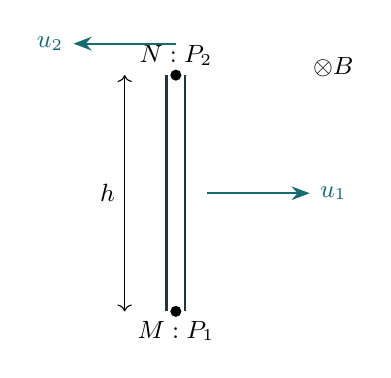
\begin{tikzpicture}[x=1cm,y=1cm]
\draw[object] (-.12,-1.5)--(-.12,1.5);\draw[object] (.12,-1.5)--(.12,1.5);\fill (0,-1.5) circle(2pt) node[below] {$M:P_1$};\fill (0,1.5) circle(2pt) node[above] {$N:P_2$};\draw[motion] (.4,0)--(1.7,0) node[right] {$u_1$};\draw[motion] (0,1.9)--(-1.3,1.9) node[left] {$u_2$};\draw[<->] (-.65,-1.5)--(-.65,1.5) node[midway,left] {$h$};\node at (2,1.6) {$\otimes B$};
\end{tikzpicture}\figcaption{图电2.11　初态两球分别位于细管两端，管向右而目标向左。}\end{minipage}\end{center}

\Needspace{6\baselineskip}\subsection*{解答}

取初始$N$为水平坐标原点，竖直坐标向上。管内球始终有水平速度$u_1$，竖直磁力$qBu_1$恒定；竖直速度引起的水平磁力由管壁抵消。记$\Omega=qB/m$，以w表示出管竖直速度。解图电2.11A采用启动后共同水平速度已为$u_1$的时刻作$t=0$，
小球相对管的初始竖直速度为零。管内轨迹在实验室系并非竖直直线，而是
$x=u_1t$、$y=-h+\tfrac12\Omega u_1t^2$；管本身也以相同的横坐标移动，所以两者相容。
\begin{center}\begin{minipage}{.97\linewidth}\centering
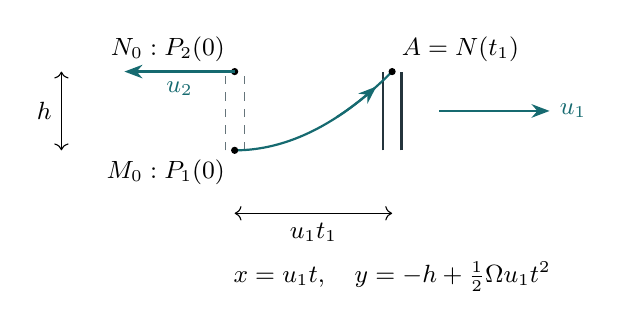
\begin{tikzpicture}[x=2cm,y=2cm,font=\small]
\draw[guide] (-.06,-.5)--(-.06,0) (.06,-.5)--(.06,0);
\draw[object] (.94,-.5)--(.94,0) (1.06,-.5)--(1.06,0);
\draw[traj,domain=0:1,samples=70] plot(\x,{\x^2/2-.5});
\draw[motion,domain=.65:.9,samples=20] plot(\x,{\x^2/2-.5});
\fill (0,-.5) circle(1.3pt) node[below left] {$M_0:P_1(0)$};
\fill (0,0) circle(1.3pt) node[above left] {$N_0:P_2(0)$};
\fill (1,0) circle(1.3pt) node[above right] {$A=N(t_1)$};
\draw[motion] (0,0)--(-.7,0) node[midway,below] {$u_2$};
\draw[motion] (1.3,-.25)--(2,-.25) node[right] {$u_1$};
\draw[<->] (-1.1,-.5)--(-1.1,0) node[midway,left] {$h$};
\draw[<->] (0,-.9)--(1,-.9) node[midway,below] {$u_1t_1$};
\node at (1,-1.3) {$x=u_1t,\quad y=-h+\tfrac12\Omega u_1t^2$};
\end{tikzpicture}
\figcaption{解图电2.11A　管内运动在地面系中的真实抛物线，示意取$u_1=\Omega=t_1=1$、$h=1/2$。虚线、实线分别为初始与出管时的管；小球始终位于移动管内，竖直初速相对管为零。}
\end{minipage}\end{center}

管内竖直动能来自移动管壁的功。管内竖直速度为$v_y$时，磁力水平分量为$-qBv_y$，
管壁须给$N_x=qBv_y$以保持$v_x=u_1$。移动管壁的功为
\[
W_{\rm wall}=\int_0^{t_1}N_xu_1\,\mathrm dt
=qBu_1\int_0^{t_1}v_y\,\mathrm dt
=qBu_1h=\frac12mw^2.
\]
磁力本身的两项功率$(-qBv_y)u_1+(qBu_1)v_y$仍相消。
管的质量足够大，可以忽略球对管速的反馈。维持管匀速的外部驱动通过运动的管壁对球做功，使球获得竖直动能。

从$M$到$N$的时间和出管竖直速度为
\[
 t_1=\sqrt{\frac{2h}{\Omega u_1}},\qquad w=\Omega u_1t_1=\sqrt{2\Omega u_1h}.
\]
出管点$A$的坐标为$(u_1t_1,0)$，出管速度$(u_1,w)$。

\begin{center}\begin{minipage}{.97\linewidth}\centering
\begin{tikzpicture}[x=1cm,y=1cm,font=\small]
\coordinate (C) at (0,1);\coordinate (A) at (1,0);\coordinate (D) at (-1,0);
\draw[guide] (C) circle({sqrt(2)});
\draw[traj] (A) arc(-45:225:{sqrt(2)});
\draw[motion] ($(C)+(85:{sqrt(2)})$) arc(85:125:{sqrt(2)});
\draw[guide] (-2.2,0)--(2.25,0);
\draw[guide] (A)--(C)--(D);
\fill (A) circle(1.6pt) node[below right] {$A$};
\fill (D) circle(1.6pt) node[below left] {$D$};
\fill (C) circle(1.4pt) node[above] {$C$};
\fill (0,0) circle(1.2pt);
\draw[guide] (0,0)--(1.65,-.55) node[right] {$N_0$};
\draw[motion] (A)--(1.7,.7) node[right] {$(u_1,w)$};
\draw[force] (D)--(-2,0) node[left] {$u_2$};
\draw ($(A)+(.35,0)$) arc(0:45:.35);
\node at (1.52,.15) {$\theta$};
\draw ($(C)+(-45:.4)$) arc(-45:-135:.4);
\node at (0,.42) {$2\theta$};
\draw[<->] (-1,-.95)--(1,-.95) node[midway,below] {$AD=2w/\Omega$};
\node at (0,2.9) {出管后沿逆时针大弧到D};
\end{tikzpicture}
\figcaption{解图电2.11B　取$w/u_1=1$，以$u_1/\Omega$为长度单位，各点严格位于半径$\sqrt2$的圆上。实线为从A到D的真实大弧，圆心角$2\pi-2\theta=3\pi/2$；下侧短弧对应相反的行进方向。}
\end{minipage}\end{center}


解图电2.11B中，正电荷在向里磁场中逆时针回转，半径$r=\sqrt{u_1^2+w^2}/\Omega$，圆心
\[
 C=(u_1t_1-w/\Omega,\ u_1/\Omega).
\]

利用$w/\Omega=u_1t_1$，圆心横坐标为0。将自由圆方程与目标运动的水平线联立：
\[
 x^2+\left(y-\frac{u_1}{\Omega}\right)^2
 =\frac{u_1^2+w^2}{\Omega^2},\qquad y=0,
\]
得到$x=\pm w/\Omega=\pm u_1t_1$。解图电2.11B的$A$是正根，$D$是负根，水平弦长应取两根之差。

设$\theta=\arctan(w/u_1)\in(0,\pi/2)$。另一处与$P_2$水平路径相交的点为$D$；$AD$是弦而非切线段，故
\[
 AD=2r\sin\theta=\frac{2w}{\Omega},\quad
 x_D=u_1t_1-\frac{2w}{\Omega}=-u_1t_1.
\]
由管内加速关系$w/\Omega=u_1t_1$，可见$D$在初始$N$左侧。\Needspace{14\baselineskip}
用分段计时的参数式写出解图电2.11B的大弧。出管后重新记局部历时$\tau=t-t_1$，令$\psi=\Omega\tau$，
则速度按向里磁场中正电荷的逆时针方向转动，位置为
\[
x(\tau)=\frac{u_1\sin\psi+w\cos\psi}{\Omega},\qquad
y(\tau)=\frac{u_1(1-\cos\psi)+w\sin\psi}{\Omega}.
\]
这里用了$u_1t_1=w/\Omega$。令$y=0$，分子可分解为
\[
2\sin\frac\psi2
\left(u_1\sin\frac\psi2+w\cos\frac\psi2\right)=0.
\]
第一类$\psi=2\pi n$回到A；第二类给$\psi=2\pi-2\theta+2\pi k$，
代入横坐标恰为$-w/\Omega$，即D。所以按逆时针出发首次到 D 时走过上方大弧。

球从$A$逆时针到$D$需转过$2\pi-2\theta$，故可相碰的时刻为
\[
 t_k=t_1+\frac{2\pi-2\theta+2\pi k}{\Omega},\qquad k=0,1,2,\ldots.
\]
$P_2$从原点向左运动，位置$-u_2t_k$，令其等于$x_D$：
\result{u_{2,k}=\frac{u_1t_1}{t_1+(2\pi-2\theta+2\pi k)/\Omega},\quad k=0,1,\ldots.}
自由圆的另一个交点 A 位于正半轴，而 $P_2$ 从开始即向左，所有相碰均发生在 D。分母随$k$增大，允许速率离散下降并趋于零，零本身不是有限时刻相碰的解。

图中 $AD$ 是连接两个真实交点的弦，半弦为 $r\sin\theta$。这与横坐标两根的差一致。

从首次出管到D的圆弧角严格在$(\pi,2\pi)$，所以每个允许碰撞时刻都晚于$t_1$。
目标从初始管口 $N_0$ 出发，走过 $N_0D=u_1t_1$；另一半弦 $N_0A$ 是管口在出管前向右走过的路程。
取解图电2.11C的 $\Omega t_1=1$，$u_{2,0}/u_1=1/(1+3\pi/2)\simeq0.1751$。
\begin{center}\begin{minipage}{.97\linewidth}\centering
\begin{tikzpicture}[x=.85cm,y=12cm,font=\small]
\draw[axis] (0,0)--(5.8,0) node[right] {$k$};
\draw[axis] (0,0)--(0,.23) node[above] {$u_{2,k}/u_1$};
\foreach \kk in {0,...,5}{
 \pgfmathsetmacro{\uk}{1/(1+1.5*pi+2*pi*\kk)}
 \draw[guide] (\kk,0)--(\kk,\uk);
 \fill[accent] (\kk,\uk) circle(1.8pt);
 \node[below] at (\kk,0) {$\kk$};
}
\node[left] at (0,.17506) {$0.1751$};
\end{tikzpicture}
\figcaption{解图电2.11C　$\Omega t_1=1$时允许目标速率的真实离散点。每增加一个k，自由段多绕一圈，同一D点的到达时刻增加$2\pi/\Omega$；目标须更慢，零只是极限值。}
\end{minipage}\end{center}

解图电2.11C 每个点都是一个不同的目标初速度。第 $k$ 点对应粒子第 $k+1$ 次经过 $D$ 时相碰。


\Needspace{18\baselineskip}

\pdfbookmark[2]{第 12 题 方波轴向磁场中的电子束聚焦}{q12}

\section*{第 12 题\quad 方波轴向磁场中的电子束聚焦}\label{q:12}

半径$R$的圆筒真空管中，两个有轴心小孔$A,A'$的隔板相距$L$。左侧电子枪连续发出电子，经$A$进入两隔板间的区域，所有电子的轴向速度分量均为$v$，横向速度各不相同。忽略电子间作用，碰壁电子被吸收。恒定轴向磁场中，使电子束在$A'$重新聚焦的最小场强为$B_0$。现令该区域磁场在$+B_0$、$-B_0$间交替，每半周期翻转一次，$t=0$起为正。
\begin{enumerate}
\item 求使非轴向电子能够在$A^{\prime}$重新聚焦的最小变化周期$T_0$。
\item 若$T=2T_0$，标出非轴向电子经$A'$射出的时间区间。
\item 求通过$A'$的电子出射方向与管轴夹角的上限。
\end{enumerate}
采用理想磁偏转模型，忽略翻转阶段的感生电场和过渡时间。

\begin{center}\begin{minipage}{.98\linewidth}\centering
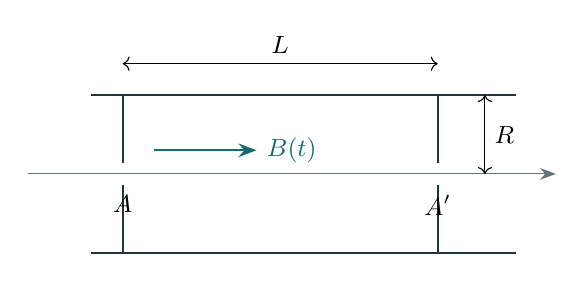
\begin{tikzpicture}[x=1cm,y=1cm]
\draw[object] (-.4,1)--(5,1);\draw[object] (-.4,-1)--(5,-1);\foreach \x/\t in {0/A,4/{A'}}{\draw[object] (\x,-1)--(\x,-.14);\draw[object] (\x,.14)--(\x,1);\node[below] at (\x,-.15) {$\t$};}\draw[axis] (-1.2,0)--(5.5,0);\draw[motion] (.4,.3)--(1.7,.3) node[right] {$B(t)$};\draw[<->] (0,1.4)--(4,1.4) node[midway,above] {$L$};\draw[<->] (4.6,0)--(4.6,1) node[midway,right] {$R$};
\end{tikzpicture}\figcaption{图电2.12　两隔板间为方波轴向磁场；两小孔均在轴线上。}\end{minipage}\end{center}

\Needspace{6\baselineskip}\subsection*{解答}

电子质量记$m_e$，电荷为$-e$。轴向运动保持匀速，解图电2.12A画出垂直管轴的实际回转轨迹。回转周期$\tau_c=2\pi m_e/(eB)$与横向速率无关，螺距$v\tau_c$。

\begin{center}\begin{minipage}{.97\linewidth}\centering
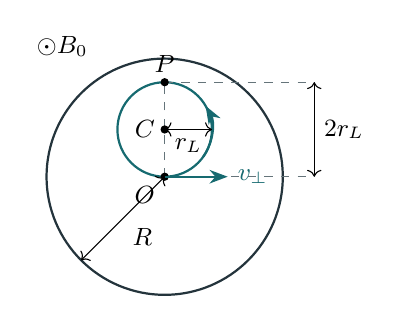
\begin{tikzpicture}[x=1cm,y=1cm,font=\small]
\coordinate (O) at (0,0);\coordinate (C) at (0,.6);\coordinate (P) at (0,1.2);
\draw[object] (O) circle(1.5);
\draw[traj] (C) circle(.6);
\draw[motion] ($(C)+(-35:.6)$) arc(-35:30:.6);
\draw[guide] (O)--(P);
\draw[<->] (O)--(225:1.5) node[midway,below right] {$R$};
\draw[<->] (C)--(.6,.6) node[midway,below] {$r_L$};
\draw[guide] (O)--(1.9,0) (P)--(1.9,1.2);
\draw[<->] (1.9,0)--(1.9,1.2) node[midway,right] {$2r_L$};
\fill (O) circle(1.5pt) node[below left] {$O$};
\fill (C) circle(1.5pt) node[left] {$C$};
\fill (P) circle(1.5pt) node[above] {$P$};
\draw[motion] (O)--(.8,0) node[right] {$v_\perp$};
\node at (-1.3,1.65) {$\odot B_0$};
\end{tikzpicture}
\figcaption{解图电2.12A　恒号磁场中的真实横截面。O是管轴，C是偏置的回转中心；圆轨道经过 O，圆心为 C，最远点 P 距轴 $2r_L$。图示轨道全在管壁以内。}
\end{minipage}\end{center}


恒定场中，$A'$重新聚焦要求$L=nv\tau_c$，于是
\[
 B_n=\frac{2\pi n m_ev}{eL},\quad B_0=\frac{2\pi m_ev}{eL}.
\]
在$B_0$下的飞行时间与回转周期相同，记$\tau=L/v=2\pi m_e/(eB_0)$。

\textbf{最短匀场时间窗。} 一次完整回转需在同一极性的半周期内完成，故$T/2\ge\tau$，得
\result{T_0=2\tau=2L/v.}
这个值对应飞行从一个恒号段的起点开始、恰转一圈。下面将有翻转的飞行按位移和方向分别计算，以确定它也是最小周期。

\begin{center}\begin{minipage}{.97\linewidth}\centering
\begin{tikzpicture}[x=1cm,y=.8cm,font=\small]
\draw[axis] (0,0)--(8.6,0) node[right] {$t/\tau$};
\draw[axis] (0,-1.3)--(0,1.5) node[above] {$B/B_0$};
\draw[traj] (0,1)--(2,1)--(2,-1)--(4,-1)--(4,1)--(6,1)--(6,-1)--(8,-1);
\foreach \xx in {1,...,8}\node[below] at (\xx,0) {$\xx$};
\foreach \aa/\bb in {0/1,2/3,4/5,6/7}\draw[line width=3pt,warm] (\aa,-1.85)--(\bb,-1.85);
\foreach \aa/\bb in {1/2,3/4,5/6,7/8}\draw[line width=3pt,accent] (\aa,-2.65)--(\bb,-2.65);
\node[left] at (0,-1.85) {入射};
\node[left] at (0,-2.65) {出射};
\draw[axis] (.5,-1.85)--(1.5,-2.65) node[pos=.5,right] {$+\tau$};
\end{tikzpicture}
\figcaption{解图电2.12B　$T=4\tau$的极性和实际透过时窗。上排为允许入射窗，下排为出射窗，两者整体相差飞行时间$\tau=L/v$；理想开关端点按连续极限计入。}
\end{minipage}\end{center}

\textbf{$T=2T_0=4\tau$。} 半周期为$2\tau$。电子若在$t_{\rm in}\in[2k\tau,(2k+1)\tau]$进入，整个飞行恰好落在同一极性时间窗中；对应出射时刻为
\result{t_{\rm out}\in[(2k+1)\tau,(2k+2)\tau],\quad k=0,1,2,\ldots.}
解图电2.12B下排绿色段标出出射窗，上排入射窗比它早$\tau$。理想瞬时开关的端点可以连续极限计入。

\begin{center}\begin{minipage}{.97\linewidth}\centering
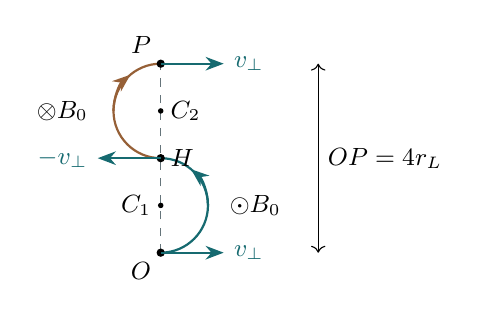
\begin{tikzpicture}[x=1cm,y=1cm,font=\small]
\coordinate (O) at (0,0);\coordinate (H) at (0,1.2);\coordinate (P) at (0,2.4);
\draw[traj] (O) arc(-90:90:.6);
\draw[motion] (.6,.6) arc(0:50:.6);
\draw[thick,warm] (H) arc(-90:-270:.6);
\draw[force] (-.6,1.8) arc(-180:-230:.6);
\draw[guide] (O)--(P);
\fill (O) circle(1.5pt) node[below left] {$O$};
\fill (H) circle(1.5pt) node[right] {$H$};
\fill (P) circle(1.5pt) node[above left] {$P$};
\fill (0,.6) circle(1pt) node[left] {$C_1$};
\fill (0,1.8) circle(1pt) node[right] {$C_2$};
\draw[motion] (O)--(.8,0) node[right] {$v_\perp$};
\draw[motion] (H)--(-.8,1.2) node[left] {$-v_\perp$};
\draw[motion] (P)--(.8,2.4) node[right] {$v_\perp$};
\node at (1.2,.6) {$\odot B_0$};
\node at (-1.25,1.8) {$\otimes B_0$};
\draw[<->] (2,0)--(2,2.4) node[midway,right] {$OP=4r_L$};
\end{tikzpicture}
\figcaption{解图电2.12C　翻转前角$\alpha=\pi$时的两段真实半圆。O至H后翻转磁场，H至P反向回转且回转中心由$C_1$变为$C_2$；末速度恢复，位置却偏离轴$4r_L$。聚焦条件由末位置给出。}
\end{minipage}\end{center}

解图电2.12C先示出翻转前后各半圈的情形。对跨越一次翻转的非轴向电子，设翻转前的回转角为$\alpha\in(0,2\pi)$。把横向位移写成复数，飞行总时间固定为$\tau$，则（略去初速度的固定相位）
\[
 \Delta z_\perp=\frac{v_\perp}{i\Omega}
 [2e^{i\alpha}-1-e^{2i\alpha}]
 =-\frac{v_\perp}{i\Omega}(e^{i\alpha}-1)^2\ne0,
 \quad\Omega=2\pi/\tau.
\]

这个位移式可以逐段得到：将进入时刻作为局部零时刻，翻转前积分$\int_0^{\alpha/\Omega}v_\perp e^{i\Omega t}\dd t$，翻转后相位从$\alpha$反向演化。两段之和为
\[
\frac{v_\perp}{i\Omega}
\left[(e^{i\alpha}-1)+e^{i\alpha}(1-e^{i\alpha})\right].
\]
若$v_\perp\ne0$，其为零只在$e^{i\alpha}=1$，即翻转落在飞行端点的极限情形。因此飞行开区间内的一次翻转会留下非零横向位移。

更短的开关周期会让飞行跨过多个恒号段，需要按可能的翻转次数继续求位移。
记恒号半周期$H=T/2$、$\beta=\Omega H$。
若$T\le\tau$，则$\beta\le\pi$。任意入射时刻之后，横向速度方向都在一个角宽不超过$\pi$的固定扇区内往返；
沿扇区中线的速度投影非负，并在非零时间内严格为正，故总位移不可能为零。

若$\tau<T<2\tau$，则$\tau/2<H<\tau$，一次飞行至多跨两次翻转。
不跨翻转无法在单个恒号段内完成一圈；跨一次已经由上式排除。
跨两次时，中段持续完整的H，前段角为$\alpha$，后段角为$2\pi-\beta-\alpha$。
逐段积分给
\[
\Delta z_\perp=\frac{v_\perp}{i\Omega}
(1-e^{-i\beta})[2e^{i\alpha}-1-e^{-i\beta}].
\]
在$\pi<\beta<2\pi$时前因子不为零；要使后因子为零，须
\[
e^{i\alpha}=\frac{1+e^{-i\beta}}2,\qquad
\left|\frac{1+e^{-i\beta}}2\right|=|\cos(\beta/2)|<1,
\]
与左边模为1矛盾。由负场开始的情形取复共轭，结论相同。
因此较短周期全部被排除，$T_0=2\tau$确为非轴向电子在理想模型中可聚焦的最小周期。
恰沿轴的电子有 $v_\perp=0$，横向始终在轴心，在任意时刻进入后均能通过。

\textbf{角度限制。} 如解图电2.12A所示，从轴心出发的回转轨迹离轴最大距离为$2r_L$，$r_L=m_ev_\perp/(eB_0)$。因碰壁即吸收，要求$2r_L<R$，即
\[
 v_\perp<\frac{eB_0R}{2m_e}=\frac{\pi Rv}{L},\qquad
 \tan\theta=\frac{v_\perp}{v}<\frac{\pi R}{L}.
\]
\result{\theta<\arctan\frac{\pi R}{L}.}
右端给可透过夹角的上确界，取到等号时轨迹恰与吸收管壁相切。

\Needspace{18\baselineskip}

\pdfbookmark[2]{第 13 题 同轴磁控管的临界磁场}{q13}

\section*{第 13 题\quad 同轴磁控管的临界磁场}\label{q:13}

无限长同轴导体间为真空，内圆柱半径$a$，外圆柱内半径$b>a$，外极相对内极电势为$V\ge0$。匀强磁场$\vect B=B\vect e_z$沿轴线向外。电子质量$m$、电荷$-e$，忽略空间电荷和感应电荷。
\begin{enumerate}
\item $B=0$，电子从内极无初速逸出，求到外极的速率，分别给出非相对论与相对论结果。
\item $V=0$，电子从内极以径向初速$v_0$逸出，求恰能触及外极的临界场，并画略强于临界时的轨道。
\item 求机械角动量$L_z$的变化率，证明$L_z-keBr^2$守恒并确定$k$。
\item 无初速电子若不能到达外极，求在最大半径$r_{\max}$处速率与$r_{\max}$的关系。
\item $V>0$时，求阻止无初速电子到达外极的临界磁场。
\item 电子从内极逸出时，沿轴、径向向外、逆时针切向初速分别为$v_z,v_r,v_\phi$，求正向磁场的临界值。
\end{enumerate}
除第(1)问相对论结果外，其余均采用非相对论近似。

\begin{center}\begin{minipage}{.98\linewidth}\centering
\begin{tikzpicture}[x=1cm,y=1cm]
\draw[object] (0,0) circle(2);\fill[accent!15] (0,0) circle(.7);\draw[object] (0,0) circle(.7);\draw[axis] (0,0)--(2.7,0) node[right] {$r$};\node[above] at (.7,0) {$a$};\node[above] at (2,0) {$b$};\node at (-.9,2.2) {$\odot B$};\node at (0,-.35) {内极};\node at (0,-2.4) {外极：$+V$};\draw[motion] (.7,0)--(1.25,0) node[above] {$v_r$};
\end{tikzpicture}\figcaption{图电2.13　电势从内极向外极升高，电子带负电。}\end{minipage}\end{center}

\Needspace{6\baselineskip}\subsection*{解答}

图电2.13中，$\vect e_r$向外、$\vect e_\phi$逆时针，$B$沿正$z$。磁力不做功，但径向速度使电子受到正切向磁力，机械角动量会改变。



\Needspace{10\baselineskip}
\textbf{(1) 电场加速。} 无初速电子电势能减少$eV$，因此
\[
 \tfrac12mv^2=eV,\quad v_{\rm nr}=\sqrt{2eV/m}.
\]
\Needspace{8\baselineskip}
相对论下动能$(\gamma-1)mc^2=eV$，从而
\[
 v_{\rm rel}=c\sqrt{1-\left(\frac{mc^2}{mc^2+eV}\right)^2}.
\]
$eV\ll mc^2$时，两式一致。

\begin{center}\begin{minipage}{.97\linewidth}\centering
\begin{tikzpicture}[x=.82cm,y=.82cm,font=\small]
\fill[accent!8] (0,0) circle(1);
\draw[object] (0,0) circle(3);\draw[object] (0,0) circle(1);
\coordinate (O) at (0,0);\coordinate (P) at (1,0);
\coordinate (C) at (1,4/3);\coordinate (T) at (1.8,2.4);
\draw[guide] (C) circle(4/3);
\draw[traj,domain=0:180-atan(.75),samples=80,variable=\t]
 plot ({1+4/3*sin(\t)},{4/3*(1-cos(\t))});
\draw[motion] ({1+4/3*sin(60)},{4/3*(1-cos(60))}) arc(-30:15:4/3);
\draw[thick,warm,domain=0:360-2*atan(33/40),samples=100,variable=\t]
 plot ({1+40/33*sin(\t)},{40/33*(1-cos(\t))});
\draw[force] ({1+40/33*sin(150)},{40/33*(1-cos(150))}) arc(60:100:40/33);
\draw[guide] (O)--(C)--(T);\draw[guide] (O)--(T);
\draw[<->] (O)--(-.707107,-.707107) node[midway,below left] {$a$};
\fill (O) circle(1.3pt) node[left] {$O$};\fill (P) circle(1.4pt) node[below right] {$P$};
\fill (C) circle(1.2pt) node[left] {$C$};\fill (T) circle(1.5pt) node[above right] {$T$};
\draw[motion] (P)--(1.8,0) node[right] {$v_0$};
\node at (-2,2.5) {$\odot B$};\node[right] at (3.2,1.7) {$V=0$};
\node[right,accent] at (3.2,1) {$B=B_{c,0}$};
\node[right,warm] at (3.2,.25) {$B=1.1B_{c,0}$};
\node[right] at (3.2,-.5) {$a:b=1:3$};
\end{tikzpicture}
\figcaption{解图电2.13A　无电场时的真实轨迹。临界弧从P走到外极切点T即停止；较强场的弧先回到内极，轨迹画到首次与导体接触处。虚圆只辅助圆心几何，$OC=\sqrt{a^2+r_L^2}$、$CT=r_L$、$OT=b$。}
\end{minipage}\end{center}

\textbf{(2) 无电场的圆轨道。} 电子径向射出，圆轨道半径$r_L=mv_0/(eB)$，圆心距轴线$\sqrt{a^2+r_L^2}$，最远半径为$\sqrt{a^2+r_L^2}+r_L$。临界时该圆与外极内切：
\[
 \sqrt{a^2+r_L^2}+r_L=b
 \ \Longrightarrow\ r_L=\frac{b^2-a^2}{2b}.
\]
\result{B_{c,0}=\frac{2bmv_0}{e(b^2-a^2)}.}
解图电2.13A中临界弧到T恰触外极；$B>B_{c,0}$时圆变小，最远位置在外极以内。等号仍触及外极，严格阻断需$B>B_c$。

\begin{center}\begin{minipage}{.97\linewidth}\centering
\begin{tikzpicture}[x=1cm,y=1cm,font=\small]
\begin{scope}
\fill (0,0) circle(1.5pt) node[below left] {$P$};
\draw[guide] (0,0)--(1.7,0) node[right] {$\boldsymbol e_r$};
\draw[guide] (0,0)--(0,1.7) node[above] {$\boldsymbol e_\phi$};
\draw[motion] (0,0)--(1.2,0) node[midway,below] {$v_r$};
\draw[motion] (0,0)--(0,1.2) node[midway,left] {$v_\phi$};
\draw[traj,->] (0,0)--(1.2,1.2) node[right] {$\boldsymbol v_\perp$};
\draw[guide] (1.2,0)--(1.2,1.2)--(0,1.2);
\node at (.5,-.7) {速度分解};
\end{scope}
\begin{scope}[xshift=5.7cm]
\fill (0,0) circle(1.5pt) node[below] {$P$};
\draw[force] (0,0)--(1.65,0) node[right] {$F_E$};
\draw[force] (0,0)--(-1.35,0) node[left] {$eBv_\phi$};
\draw[force] (0,0)--(0,1.55) node[above] {$eBv_r$};
\node at (1.2,1.3) {$\odot B$};
\node at (0,-.7) {电子受力（$v_\phi>0$）};
\end{scope}
\end{tikzpicture}
\figcaption{解图电2.13B　同一点P的速度与受力分开画。电子电场力向外；径向外速产生正切向磁力$eBv_r$，切向正速产生向内磁力$eBv_\phi$。只有切向磁力贡献轴向力矩。}
\end{minipage}\end{center}

\textbf{(3) 角动量关系。} 由解图电2.13B的切向磁力计算力矩。 电场径向，无轴向力矩。电子磁力$-e\vect v\times\vect B$的切向分量为$eBv_r$，所以
\[
 \dot L_z=eBrv_r=eBr\dot r
 =\frac{\dd}{\dd t}\left(\frac12eBr^2\right).
\]
\result{L_z-\frac12eBr^2=\text{常量},\qquad k=\frac12.}
机械角动量 $mr^2\dot\phi$ 随半径变化，扣去磁场项后等于发射时的常量。

\textbf{(4) 最大半径。} 无初速逸出时$r=a,L_z=0$。到径向转向点，$v_r=0$且$v_z=0$，全部速度为切向，故
\[
 m r_{\max}v-\tfrac12eBr_{\max}^2=-\tfrac12eBa^2,
 \quad\boxed{v=\frac{eB(r_{\max}^2-a^2)}{2mr_{\max}}}.
\]
同时电势$\varphi(r)=V\ln(r/a)/\ln(b/a)$，能量给出$v^2=2e\varphi(r_{\max})/m$，两式联立可以确定转向点。

\textbf{(5) 无初速的截止场。} 临界取$r_{\max}=b$，速率$\sqrt{2eV/m}$，代入上式：
\result{B_c=\frac{2b}{b^2-a^2}\sqrt{\frac{2mV}{e}}.}
电势的详细径向分布没有出现在最终阈值中，但它仍决定阈值以内的具体轨道。

\Needspace{18\baselineskip}
\textbf{(6) 有初速度。} 轴向速度$v_z$恒定，在能量式两端相消。临界到外极时径向速度为零，切向末速度记$v_*$。由能量与角动量
\begin{align*}
 v_*^2&=v_r^2+v_\phi^2+2eV/m,\\
 mbv_*-\tfrac12eB_cb^2&=ma v_\phi-\tfrac12eB_ca^2.
\end{align*}

第二式先解出带符号的末切向速度：
\[
v_*=\frac abv_\phi+\frac{eB_c(b^2-a^2)}{2mb}.
\]
再将它与第一式给出的速度平方比较，确定所选截止分支的正根。轴向初速未出现在此式，是因为运动中$v_z$不变，在起终能量方程中贡献相同。

在正向$B$增大导致的外侧截止分支，$v_*=+\sqrt{v_r^2+v_\phi^2+2eV/m}$，故
\result{B_c=\frac{2m}{e(b^2-a^2)}
 \left[b\sqrt{v_r^2+v_\phi^2+2eV/m}-a v_\phi\right].}
末切向速度按正向截止分支取正根；带符号的初始切向速度仍留在第二项。此式先给出端点的候选阈值，以下用径向函数证明它与从内极出发的连续可达区间相连。

\begin{center}\begin{minipage}{.97\linewidth}\centering
\begin{tikzpicture}[x=4.8cm,y=3.1cm,font=\small]
\draw[axis] (0,-.55)--(0,.72) node[above] {$F/v_V^2$};
\draw[axis] (0,0)--(1.25,0) node[right] {$x=\ln(r/a)$};
\draw[guide] (1.098612,-.5)--(1.098612,.65);
\foreach \bb/\col in {.8/warm,1/accent,1.2/muted}{
 \draw[thick,\col,domain=0:1.098612,samples=90,variable=\x]
 plot (\x,{\x/ln(3)-9/64*\bb*\bb*(exp(\x)-exp(-\x))^2});}
\fill (1.098612,0) circle(.3pt);
\node[below right] at (1.098612,-.02) {$\ell$};
\node[right,warm] at (1.1,.36) {$0.8B_c$};
\node[right,accent] at (1.1,.12) {$B_c$};
\node[right,muted] at (1.1,-.44) {$1.2B_c$};
\node[below left] at (0,0) {$0$};
\end{tikzpicture}
\figcaption{解图电2.13C　无初速、$a:b=1:3$的径向函数真曲线，$v_V=\sqrt{2eV/m}$。函数对$x=\ln(r/a)$凹，临界曲线在$0<x<\ell$内为正、仅在外极回零；更强场的外侧零点提前出现，零点之后的负值只表示禁区。}
\end{minipage}\end{center}

\textbf{从内极到外极的可达性。} 从内极出发的电子沿径向向外，只有在到达外极前 $F(r)=\dot r^2$ 始终保持正值，才会在外极首次转向。
为区别初速度与当前位置分量，以下记$u_r=v_r\ge0$、$u_\phi=v_\phi$为发射初值，$u_\phi$带符号。
任意半径的角动量关系与能量式给
\[
v_\phi(r)=\frac{au_\phi}{r}+\frac{eB(r^2-a^2)}{2mr},\qquad
\dot r^2=F(r)=u_r^2+u_\phi^2+\frac{2eV}{m}\frac{\ln(r/a)}{\ln(b/a)}-v_\phi(r)^2.
\]
如解图电2.13C，把横轴换成对数半径。令$x=\ln(r/a)$、$\ell=\ln(b/a)$、$s=eBa/(2m)$、$d=u_\phi-s$，则
\[
F(x)=u_r^2+u_\phi^2+\frac{2eV}{m\ell}x-(s e^x+d e^{-x})^2,\qquad
F''(x)=-4(s^2e^{2x}+d^2e^{-2x})\le0.
\]
在所求临界场下，$F(0)=u_r^2\ge0$、$F(\ell)=0$，因为 $x=0$ 和 $x=\ell$ 分别对应内极和外极。
凹函数位于两端连线之上，所以$0<x<\ell$内$F(x)\ge0$；非退化情形内点严格为正。
因此沿向外的分支，径向速度在到达外极前始终为正。若初速度的径向分量为零且 $F$ 在内点为正，凹性还给出 $F^{\prime}(0)>0$，电子从内极向外启动。
当$0\le B<B_c$时，外极切向速度从$(a/b)u_\phi$连续增至
$W=\sqrt{u_r^2+u_\phi^2+2eV/m}$，始终在$[-W,W]$内，故$F(\ell)\ge0$，同一凹性保证可达。
而$B>B_c$时$F(\ell)<0$，电子在外极以内转回或被内极收回。
因此等号仍触极，严格阻断取$B>B_c$。
若$V=u_r=u_\phi=0$，电子没有横向外逸运动，径向坐标保持在 $r=a$；轴向初速度只使它沿圆柱移动。


\Needspace{18\baselineskip}

\pdfbookmark[2]{第 14 题 点源到点像的磁场边界}{q14}

\section*{第 14 题\quad 点源到点像的磁场边界}\label{q:14}

质量$m$、正电荷$q$的离子从$P=(-a,0)$以相同速率$v$向$xy$上半平面的各方向射出。设计一块垂直纸面的匀强磁场$B$，使可接收的离子聚焦到$R=(a,0)$；轨道关于$y$轴对称。求磁场边界，并讨论回转半径$r=mv/(qB)$小于、等于、大于$a$时的接收角范围。出射角$\phi$从正$x$方向量起。

\begin{center}\begin{minipage}{.98\linewidth}\centering
\begin{tikzpicture}[x=1cm,y=1cm]
\draw[axis] (-2.8,0)--(2.8,0) node[right] {$x$};\draw[axis] (0,-.2)--(0,2.2) node[above] {$y$};\fill (-1.8,0) circle(2pt) node[below] {$P$};\fill (1.8,0) circle(2pt) node[below] {$R$};\foreach \ang in {20,40,60,80,110,145}\draw[motion] (-1.8,0)--++(\ang:.8);\node[below] at (-.9,0) {$a$};\node[below] at (.9,0) {$a$};\node at (1.8,1.8) {$\odot B$};
\end{tikzpicture}\figcaption{图电2.14　从P发射的上半平面点源，设计左右对称场区。}\end{minipage}\end{center}

\Needspace{6\baselineskip}\subsection*{解答}

轨道由入射直线、半径$r$的圆弧和出射直线组成。解图电2.14A中，圆心在$y$轴上，写作$C=(0,b)$。右边界点$A=(x,y)$处的切线必须通过像点$R$，因此半径$CA$与$AR$垂直：
\[
 x(a-x)-y(y-b)=0,\qquad x^2+(y-b)^2=r^2.
\]
\begin{center}\begin{minipage}{.98\linewidth}\centering
\begin{tikzpicture}[x=1cm,y=1cm]
\draw[axis] (-3.2,0)--(3.2,0) node[right] {$x$};\draw[axis] (0,-.3)--(0,3) node[above] {$y$};
\coordinate (P) at (-2.625,0);\coordinate (R) at (2.625,0);\coordinate (C) at (0,1);\coordinate (A) at (1.2,1.9);\coordinate (D) at (-1.2,1.9);
\draw[motion] (P)--(D);\draw[traj,->] (D) arc(143.13:36.87:1.5);\draw[motion] (A)--(R);
\draw[guide] (C)--(A) node[midway,below] {$r$};\draw[guide] (A)--(1.2,0);\draw[guide] (0,1.9)--(A);
\foreach \p in {P,R,C,A}\fill (\p) circle(1.5pt);\node[below] at (P) {$P$};\node[below] at (R) {$R$};\node[left] at (C) {$C=(0,b)$};\node[above right] at (A) {$A=(x,y)$};\node[below] at (1.2,0) {$x$};\node[left] at (0,1.9) {$y$};\node at (-1.3,-.55) {$a$};\node at (1.3,-.55) {$a$};
\end{tikzpicture}\figcaption{解图电2.14A　入射与出射直线分别切于左右端，CA垂直AR；圆心在y轴上。}\end{minipage}\end{center}
由第一式$y-b=x(a-x)/y$，代入第二式，得
\[
 (r^2-x^2)y^2=x^2(a-x)^2.
\]
取第一象限的实支为右边界，左边界由镜像得到：
\result{y=\frac{|x|(a-|x|)}{\sqrt{r^2-x^2}}.}
只取$y\ge0$且$|x|<r$的支。在$r<a$时，$0\le|x|<r$；在$r\ge a$时，实际上半平面边界用$0\le|x|\le a$。磁场取图B浅色所示、两支边界上方的连通区域，方向选为使正离子由入射方向转向出射方向的纸面向外。

\begin{center}\begin{minipage}{.97\linewidth}\centering
\begin{tikzpicture}[x=1cm,y=1cm,font=\small]
\foreach \rr/\sx/\lab in {.7/-3/{r<a},1/0/{r=a},1.5/3/{r>a}}{
\begin{scope}[shift={(\sx,0)}]
\begin{scope}\clip (-1.15,0) rectangle(1.15,2.5);
\ifdim\rr pt<1pt
 \fill[accent!12] (-.7,0) rectangle(.7,2.5);
 \fill[white] (-.6999,0)--plot[domain=-.6999:0,samples=100](\x,{-\x*(1+\x)/sqrt(\rr*\rr-\x*\x)})
 --plot[domain=0:.6999,samples=100](\x,{\x*(1-\x)/sqrt(\rr*\rr-\x*\x)})--(.6999,0)--cycle;
 \draw[traj,domain=0:.6999,samples=100] plot(\x,{\x*(1-\x)/sqrt(\rr*\rr-\x*\x)});
 \draw[traj,domain=-.6999:0,samples=100] plot(\x,{-\x*(1+\x)/sqrt(\rr*\rr-\x*\x)});
 \draw[guide] (-.7,0)--(-.7,2.5) (.7,0)--(.7,2.5);
\else
 \fill[accent!12] (-1,0) rectangle(1,2.5);
 \ifdim\rr pt=1pt
  \fill[white] (-1,0)--plot[domain=-1:0,samples=100](\x,{-\x*sqrt((1+\x)/(1-\x))})
  --plot[domain=0:1,samples=100](\x,{\x*sqrt((1-\x)/(1+\x))})--cycle;
  \draw[traj,domain=0:1,samples=100] plot(\x,{\x*sqrt((1-\x)/(1+\x))});
  \draw[traj,domain=-1:0,samples=100] plot(\x,{-\x*sqrt((1+\x)/(1-\x))});
 \else
  \fill[white] (-1,0)--plot[domain=-1:0,samples=100](\x,{-\x*(1+\x)/sqrt(\rr*\rr-\x*\x)})
  --plot[domain=0:1,samples=100](\x,{\x*(1-\x)/sqrt(\rr*\rr-\x*\x)})--cycle;
  \draw[traj,domain=0:1,samples=100] plot(\x,{\x*(1-\x)/sqrt(\rr*\rr-\x*\x)});
  \draw[traj,domain=-1:0,samples=100] plot(\x,{-\x*(1+\x)/sqrt(\rr*\rr-\x*\x)});
 \fi
\fi
\node at (0,1.65) {$\odot B$};\end{scope}
\draw[axis] (-1.25,0)--(1.25,0);\draw[axis] (0,-.1)--(0,2.6);
\fill (-1,0) circle(1.3pt) node[below] {$P$};\fill (1,0) circle(1.3pt) node[below] {$R$};
\node at (0,-.65) {$\lab$};\end{scope}}
\end{tikzpicture}
\figcaption{解图电2.14B　$a=1$的三类边界，浅色一侧为磁场；有场区域为中轴上方相连的浅色部分。左右范围分别止于$|x|<r$或$|x|\le a$；图顶是裁切边，场区仍向上延伸。}
\end{minipage}\end{center}


\textbf{$r<a$。} 边界在$|x|\to r$时升至无穷。$0<\phi<\pi/2$的入射线可进入场区并聚焦；向左的射线不会进入该设计区域。角度端点按相切极限理解。

\textbf{$r=a$。} 代入可写成$y=|x|\sqrt{(a-|x|)/(a+|x|)}$，所以在$|x|\to a$时$y\to0$，边界在 $P,R$ 回到横轴。此时接收极限为垂直方向。

\textbf{$r>a$。} 场区在$P,R$处落回$x$轴。最陡可接受入射线与左边界在$P$相切。对左支
\[
 y=-\frac{x(a+x)}{\sqrt{r^2-x^2}},\qquad
 y'(-a)=\frac a{\sqrt{r^2-a^2}}.
\]

将左端附近的边界写成一阶展开。令左端$x=-a+\varepsilon$、$\varepsilon>0$，则
\[
y=\frac{(a-\varepsilon)\varepsilon}
{\sqrt{r^2-(-a+\varepsilon)^2}}
=\frac{a}{\sqrt{r^2-a^2}}\varepsilon+O(\varepsilon^2).
\]
因此解图电2.14B中$r>a$的左端切线斜率确为上述值，它直接决定能从$P$进入该场区的极限方向。

因而
\result{\phi_{\max}=\arctan\frac a{\sqrt{r^2-a^2}}
 =\arcsin\frac a r<\frac\pi2.}
此角把入场切点移到 P。继续增大角度时，代数切点落在入射射线的反向延长线上。

\begin{center}\begin{minipage}{.97\linewidth}\centering
\begin{tikzpicture}[x=2.4cm,y=2.4cm,font=\small]
\draw[axis] (-1.15,0)--(1.15,0) node[right] {$x/a$};
\draw[axis] (0,-.35)--(0,1.35) node[above] {$y/a$};
\foreach \ph/\col in {30/warm,60/accent}{
 \pgfmathsetmacro{\bb}{(sin(\ph)-.7)/cos(\ph)}
 \pgfmathsetmacro{\dx}{.7*sin(\ph)}\pgfmathsetmacro{\dy}{(1-\dx)*tan(\ph)}
 \draw[thick,\col,->] (-1,0)--(-\dx,\dy);
 \draw[thick,\col,domain=90+\ph:90-\ph,samples=65,variable=\t]
 plot ({.7*cos(\t)},{\bb+.7*sin(\t)});
 \draw[thick,\col,->] (\dx,\dy)--(1,0);
 \fill[\col] (0,\bb) circle(.55pt);
}
\fill (-1,0) circle(.6pt) node[below] {$P$};\fill (1,0) circle(.6pt) node[below] {$R$};
\node[right,warm] at (1.2,.55) {$\phi=30^\circ$};
\node[right,accent] at (1.2,.95) {$\phi=60^\circ$};
\node at (-.95,1.05) {$r/a=0.7$};
\end{tikzpicture}
\figcaption{解图电2.14C　同一半径$r=0.7a$下两条真正聚焦轨道。切点随发射角改变，两个圆心高度也不同；圆弧均按正离子在向外磁场中的顺时针转向连接两段直线。}
\end{minipage}\end{center}

\textbf{通过入场距离求接收角域。} 解图电2.14C中，给定初始方向$0<\phi<\pi/2$，把左切点记D。
顺时针圆弧开始处的半径方向与入射速度垂直，因此
\[
D=(-r\sin\phi,(a-r\sin\phi)\tan\phi),\qquad
C=\left(0,\frac{a\sin\phi-r}{\cos\phi}\right).
\]
从P到D的直线长度为$\lambda=(a-r\sin\phi)/\cos\phi$。
入场必须发生在从P出发的正向射线上，故条件就是$r\sin\phi\le a$。
这个条件给出前面三种角域：$r<a$时所有锐角都可接收，$r=a$时垂直方向成为极限，$r>a$时只到$\arcsin(a/r)$。
等号时入场直线长度为零，即切点退到 P；若分子为负，切点在反向延长线上。

圆弧的右端是D关于y轴的镜像，离场速度方向为$-\phi$，沿切线恰到R。
把$A_x=r\sin\phi$及$A_y=(a-r\sin\phi)\tan\phi$代入右边界式，等式逐项成立。
解图电2.14B 的浅色区域在边线上方。沿解图电2.14C 的圆弧取 $u=|x|$，比较圆弧高度 $y_{\rm arc}=b+\sqrt{r^2-u^2}$ 与边线高度 $y_{\rm edge}=u(a-u)/\sqrt{r^2-u^2}$：
\[
y_{\rm arc}-y_{\rm edge}=b+\frac{r^2-au}{\sqrt{r^2-u^2}},
\qquad
\frac{\dd}{\dd u}(y_{\rm arc}-y_{\rm edge})
=\frac{r^2(u-a)}{(r^2-u^2)^{3/2}}.
\]
当 $0\le u\le r\sin\phi\le a$ 时，高度差随 $u$ 减小而增大，在两端切点处为零，因此整段圆弧都在有场区。入射直线在左边线以下。具体地，左半面入口前 $u>r\sin\phi$ 时，直线为 $y=(a-u)\tan\phi$，而边线斜率比值 $y_{\rm edge}/(a-u)=u/\sqrt{r^2-u^2}$ 大于 $\tan\phi$。离场直线由镜像得到，同样处在零场区。

端点还要按题设的理想边界说明：$\phi=0$是沿x轴直接从P到R的退化轨道。
$r=a,\phi=\pi/2$时，P、R正是圆弧两端，入场直线长度趋零，圆弧成为上半圆；若把边界赋予内侧磁场值，可包含这一极限方向。
$r<a$ 时垂直射线始终保持 $x=-a<-r$，在场区的横向范围以外。
当$r>a$且角度趋近上限时，两段直线同样缩为零，圆心在$C=(0,-\sqrt{r^2-a^2})$，对应的上圆弧仍从P到R。
这些端点的差异也是三类边界不能合并略去的原因。


\Needspace{18\baselineskip}

\pdfbookmark[2]{第 15 题 电子束先会聚再扩束的四区磁场}{q15}

\section*{第 15 题\quad 电子束先会聚再扩束的四区磁场}\label{q:15}

一束稀疏电子从$x$负半轴远处、$-H<y<H$的条带中，以同一速率$v$沿正$x$方向平行入射。设计有限的分区匀强磁场，使所有电子先通过原点$O$，再在远处恢复为沿正$x$方向、同一速率$v$的平行束，出射条带为$-2H<y<2H$。忽略电子间相互作用，给出一种场区边界及各区磁场。

\begin{center}\begin{minipage}{.98\linewidth}\centering
\begin{tikzpicture}[x=1cm,y=1cm]
\draw[axis] (-3.2,0)--(4.3,0) node[right] {$x$};\draw[axis] (0,-2.4)--(0,2.4) node[above] {$y$};\foreach \y in {-.8,-.4,.4,.8}\draw[motion] (-3,\y)--(-1.9,\y);\foreach \y in {-1.6,-.8,.8,1.6}\draw[motion] (2.1,\y)--(3.2,\y);\draw[<->] (-2.9,-1)--(-2.9,1) node[pos=.70,left] {$2H$};\draw[<->] (3.1,-2)--(3.1,2) node[pos=.60,right] {$4H$};\node[below left] at (0,0) {$O$};
\end{tikzpicture}\figcaption{图电2.15　入射束半宽H，要求过O后成为半宽2H的平行束。}\end{minipage}\end{center}

\Needspace{6\baselineskip}\subsection*{解答}

解图电2.15A将轨道按$x$轴两侧和$y$轴两侧分成四区：上半束在左侧被向下偏折，过$O$后进入右下方；下半束则镜像进入右上方。左右两部分的回转半径可不同，速率因磁力不做功保持$v$。

\begin{center}\begin{minipage}{.97\linewidth}\centering
\begin{tikzpicture}[x=1cm,y=1cm,font=\small]
\foreach \sy in {-1,1}{\begin{scope}[yscale=\sy]
\fill[accent!12] (0,0) arc(180:90:2)--(2,2) arc(0:-90:2)--cycle;
\fill[warm!12] (0,0) arc(-90:-180:1)--(-1,1) arc(90:0:1)--cycle;
\draw[object] (0,0) arc(180:90:2) arc(0:-90:2);
\draw[object] (0,0) arc(-90:-180:1) arc(90:0:1);
\end{scope}}
\draw[axis] (-1.6,0)--(2.8,0) node[right] {$x/H$};\draw[axis] (0,-2.4)--(0,2.5) node[above] {$y/H$};
\node at (1,1.15) {$\otimes B_1$};\node at (1,-1.15) {$\odot B_1$};
\node[left] at (-1.15,.7) {$\otimes2B_1$};\node[left] at (-1.15,-.7) {$\odot2B_1$};
\node[below left] at (0,0) {$O$};\node[right] at (2,2) {$(2,2)$};\node[left] at (-1,1) {$(-1,1)$};
\end{tikzpicture}
\figcaption{解图电2.15A　四片有场叶片都填出，叶片外无场。左半径 $H$、右半径 $2H$，上方场向里，下方场向外。右侧一条边线连接出场点，另一条是最陡轨迹的极限圆弧。左侧为对应的逆过程。}
\end{minipage}\end{center}


\begin{center}\begin{minipage}{.97\linewidth}\centering
\begin{tikzpicture}[x=1.3cm,y=1.3cm,font=\small]
\coordinate (O) at (0,0);\coordinate (C) at (1.7320508,-1);
\draw[guide] (C) circle(2);\draw[traj,->] (O) arc(150:90:2);
\draw[object,domain=0:60,samples=60,variable=\t] plot({2*sin(\t)},{2*(1-cos(\t))});
\draw[motion] (O)--(.6,1.03923) node[above left] {$v$};
\draw[motion] (1.7320508,1)--(2.6,1) node[right] {$v$};
\draw[guide] (O)--(C)--(1.7320508,1);
\fill (O) circle(1pt) node[below left] {$O$};\fill (C) circle(1pt) node[right] {$C$};
\fill (1.7320508,1) circle(1pt) node[above right] {$S$};
\draw[axis] (-.4,0)--(2.7,0) node[right] {$x$};
\node at (-.7,1.5) {$\theta=60^\circ$};\node at (2.7,-.6) {$\otimes B_1$};
\end{tikzpicture}
\figcaption{解图电2.15B　右上准直过程，$r_1=2H$、$\theta=60^\circ$。真实回转圆心C在下方；S处速度水平。黑色较低圆弧连接不同轨迹的出场点 S，彩色弧是这一粒电子的路径。}
\end{minipage}\end{center}

如解图电2.15B，先从$O$向第一象限反推出射过程。设离开$O$的方向与正$x$轴夹角为$\theta$，右上区半径$r_1$，电子沿顺时针圆弧转到水平。其圆心为$(r_1\sin\theta,-r_1\cos\theta)$，变成水平时的位置$S$满足
\[
 x_S=r_1\sin\theta,\qquad y_S=r_1(1-\cos\theta).
\]
消去$\theta$，出射边界为$x^2+(y-r_1)^2=r_1^2$。而最陡射线$\theta\to\pi/2$的圆弧为$(x-r_1)^2+y^2=r_1^2$。两圆之间的第一象限叶片构成场区；它们在$(0,0)$和$(r_1,r_1)$相交。为得到出射上边界$y=2H$，取$r_1=2H$，于是
\[
 B_{\rm I}=\frac{mv}{2eH},\qquad\text{方向向里}.
\]
右下区是上区关于$x$轴的镜像，场大小相同、方向向外，保证负$y$出射束也变为水平向右。

左侧用同样的几何关系反推会聚过程，但入射半宽只有$H$，所以$r_2=H$。左上区的两条边界为
\[
 x^2+(y-H)^2=H^2,\qquad (x+H)^2+y^2=H^2,
\]
取第二象限两弧之间的叶片。其磁场向里，大小$mv/(eH)=2B_{\rm I}$；左下区镜像，方向向外。

因此四区可统一写为
\result{|B_{\rm II}|=|B_{\rm III}|=\frac{mv}{eH},\quad
 |B_{\rm I}|=|B_{\rm IV}|=\frac{mv}{2eH}.}
第一、二象限场向里，第三、四象限场向外，叶片以外为零场。沿轨道连续性，$O$处的离开方向由左侧入射弧决定；过$O$不需要人为折转速度。

入射高度$y_0>0$对应$y_0=H(1-\cos\theta)$，出射高度为$-2H(1-\cos\theta)=-2y_0$，下半束同理，故此设计确实把条带放大两倍并上下反转。
按这一映射追踪经过 $O$ 的速度：左上方来的电子到$O$时指向右下，在右下场内继续沿该方向进入圆弧，随后才转成水平；边界处没有让速度突然翻转的冲量。取$y_0=H/2$，有$\theta=60^\circ$，出射高度应为$-H$，可在解图电2.15A的左右叶片上逐段跟踪。

$y_0=0$的轴向电子作直线运动，是连续极限。

\begin{center}\begin{minipage}{.97\linewidth}\centering
\begin{tikzpicture}[x=1.55cm,y=1.55cm,font=\small]
\draw[axis] (-1.6,0)--(2.6,0) node[right] {$x/H$};\draw[axis] (0,-1.4)--(0,1) node[above] {$y/H$};
\draw[motion] (-1.5,.5)--(-.8660254,.5);
\draw[traj,->] (-.8660254,.5) arc(90:30:1);
\draw[traj,->] (0,0) arc(210:270:2);
\draw[motion] (1.7320508,-1)--(2.5,-1);
\draw[motion] (0,0)--(.42,-.72746) node[right] {$\boldsymbol v_O$};
\fill (-.8660254,.5) circle(1pt) node[above] {$A$};\fill (0,0) circle(1pt) node[above left] {$O$};
\fill (1.7320508,-1) circle(1pt) node[below] {$S$};
\node at (-1.5,.9) {$y_0=H/2$};\node at (1,-1.55) {$y_{\rm out}=-H$};
\end{tikzpicture}
\figcaption{解图电2.15C　任取$y_0=H/2$的一条完整射线。入场A后顺时针走到O，再在右下区逆时针走到S，O处两弧切向连续；末高度为$-2y_0$，末速度仍向右。}
\end{minipage}\end{center}

\textbf{沿任意高度的轨迹通过叶片。} 解图电2.15A给出一种有限场区，而不要求设计唯一。
第一象限的叶片是两个圆盘的交集：$x^2+(y-r_1)^2\le r_1^2$与$(x-r_1)^2+y^2\le r_1^2$；
两个圆盘条件同时成立的位置才属于叶片。两个端点O和$(r_1,r_1)$之间，一条边界给出S的轨迹，另一条由最陡射线的四分之一圆限定。
电子在前一条边界到达S时切线已水平，进入叶片外的零场区域后，粒子沿这条水平切线继续前进。

这个叶片确实容纳所有$0\le\theta\le\pi/2$的回转弧。
把从O出发后的转角记为$\psi$，$0\le\psi\le\theta$，并令$\eta=\theta-\psi$，则右上弧上任一点为
\[
x=r_1(\sin\theta-\sin\eta),\qquad
y=r_1(\cos\eta-\cos\theta).
\]
此时$x^2+y^2=4r_1^2\sin^2(\psi/2)$，而
$y=2r_1\sin(\theta-\psi/2)\sin(\psi/2)$、
$x=2r_1\cos(\theta-\psi/2)\sin(\psi/2)$。
由于$\psi/2\le\theta-\psi/2\le\pi/2-\psi/2$，有
$\sin(\theta-\psi/2)\ge\sin(\psi/2)$且
$\cos(\theta-\psi/2)\ge\sin(\psi/2)$，从而同时满足两个圆盘不等式。
因此各个入射角对应的整段圆弧都在这片场区内。

对左上方任意入射高度$0<y_0<H$，令$\cos\theta=1-y_0/H$。
其入口与左回转圆心分别为
\[
A=(-H\sin\theta,y_0),\qquad C_L=(-H\sin\theta,-H\cos\theta).
\]
电子从A以水平速度进入，在向里磁场中顺时针转过$\theta$，到O时的速度为
$\boldsymbol v_O=v(\cos\theta,-\sin\theta)$。
随后右下场向外，回转方向改为逆时针，圆心变成
$C_R=(2H\sin\theta,2H\cos\theta)$，同样转过$\theta$后，在
$S=(2H\sin\theta,-2y_0)$恢复向右水平。
解图电2.15C把这一过程逐段画出，图B的上方准直弧正是它关于x轴的镜像。
下半入射束再作镜像，得到同一个映射$y_{\rm out}=-2y_0$，左右圆弧在焦点沿同一条切线衔接。

从 O 反推得到几何轮廓后，沿实际入射方向用电子的洛伦兹力确定各叶片场向。
在O附近，速度连续而曲率因场向和大小改变：左上弧转到右下弧时，切线没有跳变。
磁力始终与速度垂直，故电子的速率、动能在会聚、穿焦和扩束各段都不变。
轴线$y_0=0$取直行极限，开区间边缘$|y_0|\to H$给出叶片的最陡极限弧；连续束的边缘按这个极限确定。
四片场区均为有限圆盘的交集。电子过 O 后，按 $y_{\rm out}=-2y_0$ 映射到加宽的平行束。


\Needspace{18\baselineskip}

\pdfbookmark[2]{第 16 题 环形磁场中的电子束聚焦与漂移}{q16}

\section*{第 16 题\quad 环形磁场中的电子束聚焦与漂移}\label{q:16}

平均半径$R$的螺绕环中，从场线上的点源$P$沿磁力线方向射入小孔径角$2\alpha_0$的电子束，$\alpha_0\ll1$。电子均经电压$U_0$加速，忽略相互作用。磁场大小按理想模型取常量$B$。
\begin{enumerate}
\item 求使电子沿半径$R$的圆形轴线运动所需的垂直环平面匀强偏转场$B_1$。
\item 忽略$B_1$和场线弯曲，要求电子束每绕环$\pi/2$圆周角聚焦一次，求$B$。
\item 不加$B_1$，电子沿环切线发射。证明其径向偏离有界，并确定垂直环面的漂移方向；保留径向转向方程及其精确求根形式。
\end{enumerate}
给定$e/m=1.76\times10^{11}\,\mathrm{C/kg}$、$U_0=3\,\mathrm{kV}$、$R=50\,\mathrm{mm}$。取环面为$xy$面、环形场沿$+\phi$方向。

\begin{center}\begin{minipage}{.98\linewidth}\centering
\begin{tikzpicture}[x=1cm,y=1cm]
\draw[object] (0,0) circle(2);\draw[object] (0,0) circle(1.4);\draw[guide] (0,0) circle(1.7);\fill (1.7,0) circle(2pt) node[right] {$P$};\draw[motion] (1.7,0)--(1.7,1) node[right] {$v_0,B$};\draw[<->] (0,0)--(-1.2,1.2) node[midway,left] {$R$};\foreach \ang in {90,180,270}\fill (\ang:1.7) circle(1.6pt);
\end{tikzpicture}\figcaption{图电2.16　沿环形轴线每四分之一周设置一个近轴焦点。}\end{minipage}\end{center}

\Needspace{6\baselineskip}\subsection*{解答}

先由加速关系得$v_0=\sqrt{2eU_0/m}$。

\begin{center}\begin{minipage}{.97\linewidth}\centering
\begin{tikzpicture}[x=1cm,y=1cm,font=\small]
\draw[guide] (0,0) circle(1.5);\fill (1.5,0) circle(1.4pt) node[below right] {$P$};
\draw[motion] (1.5,0)--(1.5,1) node[right] {$v_0,\ B\boldsymbol e_\phi$};
\draw[force] (1.5,0)--(.5,0) node[midway,below] {$F_{B_1}$};
\draw[<->] (0,0)--(-1.06,1.06) node[midway,above right] {$R$};
\node at (-1.4,-1.5) {$\odot B_1$};\node[below] at (0,0) {$O$};
\begin{scope}[xshift=5cm]
\draw[axis] (0,0)--(1.9,0) node[right] {$\boldsymbol e_r$};
\draw[axis] (0,-1.3)--(0,1.2) node[above] {$\boldsymbol e_z$};
\fill (0,0) circle(1.3pt);
\draw[motion] (0,0)--(1.1,0) node[above] {$v_r>0$};
\draw[force] (0,0)--(0,-1) node[right] {$F_z=-eBv_r$};
\draw[force] (0,0)--(-1.4,0);
\node[anchor=east] at (-.2,-.5) {$F_r=eBv_z<0$};
\node at (1.2,.9) {$\otimes\boldsymbol B_\phi$};
\end{scope}
\end{tikzpicture}
\figcaption{解图电2.16A　左为需补的向心力，右为无$B_1$时的局部$r,z$截面。按右手柱坐标，$+\phi$场指向纸内；外向$v_r$产生负z力，随后$v_z<0$产生向内径向力。}
\end{minipage}\end{center}


\textbf{(1) 偏转场。} 沿轴线的速度与环形场平行，环形场不能直接提供向心力。另加$B_1$垂直环面向外，使电子受到向心磁力。由
\[
 ev_0B_1=mv_0^2/R
\]
可得$B_1=\sqrt{2mU_0/e}/R=3.69\times10^{-3}\,\mathrm T$。

\textbf{(2) 近轴聚焦。} 把小段弯曲场线展直，电子速度分量为$v_\parallel=v_0\cos\alpha$、$v_\perp=v_0\sin\alpha$。回转周期$\tau_c=2\pi m/(eB)$，螺距$b=v_\parallel\tau_c$。每四分之一环聚焦一次，要求$b=2\pi R/4$，因此
\[
 B=\frac4R\sqrt{\frac{2mU_0}{e}}\cos\alpha
 \simeq\frac4R\sqrt{\frac{2mU_0}{e}}
 =1.48\times10^{-2}\,\mathrm T.
\]
不同$\alpha$的$\cos\alpha$略有差别，严格共焦只在近轴极限成立，有限孔径会产生二阶散焦。

\textbf{(3) 无偏转场的径向约束。} 柱坐标速度为$(v_r,v_\phi,v_z)$，初态$(0,v_0,0)$、$r=R$。磁力不做功，也无$\phi$分量，故
\[
 v_r^2+v_\phi^2+v_z^2=v_0^2,\qquad rv_\phi=Rv_0.
\]
电子受轴向力$F_z=-eBv_r$，积分得$v_z=-\Omega(r-R)$，$\Omega=eB/m$。于是
\[
 v_r^2=v_0^2-\frac{R^2v_0^2}{r^2}-\Omega^2(r-R)^2.
\]
令$s=r/R$、$A=\Omega R/v_0$，径向转向方程为
\[
 1=s^{-2}+A^2(s-1)^2.
\]
\begin{center}\begin{minipage}{.97\linewidth}\centering
\begin{tikzpicture}[x=8cm,y=4cm,font=\small]
\draw[axis] (.88,.8)--(1.21,.8) node[right] {$s=r/R$};
\draw[axis] (.9,.78)--(.9,1.3);
\draw[guide] (.9,1)--(1.19,1) node[right] {$1$};
\draw[traj,domain=.9:1.18,samples=100,variable=\x] plot(\x,{1/\x^2+16*(\x-1)^2});
\draw[guide] (1,.8)--(1,1);\draw[guide] (1.10740296,.8)--(1.10740296,1);
\node[below] at (1,.8) {$1$};\node[below] at (1.10740296,.8) {$s_*$};
\node at (1.055,1.4) {$f(s)=s^{-2}+16(s-1)^2$};
\end{tikzpicture}
\figcaption{解图电2.16B　$A=4$的真实转向函数。$f\le1$才可达，允许区是$1\le s\le s_*$；两根是径向转向点，电子的切向速度并未消失。}
\end{minipage}\end{center}

解图电2.16B显示$s=1$为一个根；$0<s<1$时右端大于1，径向速度平方为负，因此允许区从 $s=1$ 开始。$s>1$时转向方程约去$s-1$后为
\[
 A^2s^2(s-1)=s+1.
\]

为把唯一性证明写完整，设
\[
g(s)=\frac{s^2(s-1)}{s+1},\qquad
g'(s)=\frac{2s(s^2+s-1)}{(s+1)^2}>0\quad(s>1).
\]
转向条件是$A^2g(s)=1$，而$g(1)=0$、$g(s)\to\infty$。故恰有一个外侧根，与解图电2.16B的允许径向区间一致。

因此$R\le r\le Rs_*$，径向偏离有限，而$v_z=-\Omega(r-R)\le0$，总体向负$z$漂移。

\textbf{精确求根。} 三次方程$s^3-s^2-s/A^2-1/A^2=0$，令$s=u+1/3$，可写成$u^3+pu+q=0$，其中
\[
 p=-\left(\frac13+\frac1{A^2}\right),\quad
 q=-\left(\frac2{27}+\frac4{3A^2}\right),\quad
 \Delta=(q/2)^2+(p/3)^3.
\]
当$\Delta\ge0$，
\[
 s_*=\frac13+\sqrt[3]{-q/2+\sqrt\Delta}+\sqrt[3]{-q/2-\sqrt\Delta}.
\]
当$\Delta<0$，取最大的实根
\[
 s_*=\frac13+2\sqrt{-p/3}\cos\left[\frac13\arccos\left(\frac{3q}{2p}\sqrt{-3/p}\right)\right].
\]
其他实根即使存在，也不在$s>1$的可达分支上。这里按题给恒定的环形场积分。若改取 $B\propto1/r$，轴向速度由径向积分得到对数函数。

\begin{center}\begin{minipage}{.97\linewidth}\centering
\begin{tikzpicture}[x=28cm,y=3.7cm,font=\small]
\draw[axis] (0,0)--(.14,0) node[right] {$(r-R)/R$};
\draw[axis] (0,-.85)--(0,.08) node[above] {$z/R$};
\draw[traj] plot coordinates {(0.000000000,0.000000000) (0.000159714,-0.000003808) (0.000637888,-0.000030434) (0.001431621,-0.000102560) (0.002536098,-0.000242588) (0.003944625,-0.000472513) (0.005648670,-0.000813781) (0.007637925,-0.001287167) (0.009900364,-0.001912646) (0.012422334,-0.002709273) (0.015188632,-0.003695072) (0.018182611,-0.004886930) (0.021386285,-0.006300490) (0.024780442,-0.007950068) (0.028344767,-0.009848565) (0.032057967,-0.012007394) (0.035897905,-0.014436413) (0.039841738,-0.017143873) (0.043866051,-0.020136368) (0.047947003,-0.023418804) (0.052060468,-0.026994368) (0.056182181,-0.030864520) (0.060287876,-0.035028980) (0.064353431,-0.039485740) (0.068355009,-0.044231074) (0.072269191,-0.049259568) (0.076073114,-0.054564151) (0.079744597,-0.060136141) (0.083262269,-0.065965298) (0.086605686,-0.072039886) (0.089755448,-0.078346745) (0.092693304,-0.084871367) (0.095402251,-0.091597984) (0.097866632,-0.098509658) (0.100072218,-0.105588383) (0.102006288,-0.112815189) (0.103657694,-0.120170252) (0.105016926,-0.127633011) (0.106076161,-0.135182281) (0.106829306,-0.142796382) (0.107272029,-0.150453261) (0.107401786,-0.158130619) (0.107217830,-0.165806038) (0.106721220,-0.173457112) (0.105914809,-0.181061575) (0.104803236,-0.188597429) (0.103392895,-0.196043071) (0.101691906,-0.203377417) (0.099710064,-0.210580022) (0.097458793,-0.217631204) (0.094951082,-0.224512149) (0.092201411,-0.231205031) (0.089225676,-0.237693107) (0.086041103,-0.243960819) (0.082666149,-0.249993888) (0.079120403,-0.255779392) (0.075424476,-0.261305851) (0.071599889,-0.266563289) (0.067668949,-0.271543299) (0.063654626,-0.276239095) (0.059580419,-0.280645550) (0.055470225,-0.284759235) (0.051348201,-0.288578440) (0.047238623,-0.292103185) (0.043165742,-0.295335230) (0.039153646,-0.298278059) (0.035226112,-0.300936873) (0.031406465,-0.303318556) (0.027717437,-0.305431638) (0.024181028,-0.307286252) (0.020818373,-0.308894073) (0.017649603,-0.310268251) (0.014693728,-0.311423337) (0.011968510,-0.312375199) (0.009490355,-0.313140925) (0.007274203,-0.313738725) (0.005333433,-0.314187823) (0.003679779,-0.314508341) (0.002323247,-0.314721177) (0.001272054,-0.314847883) (0.000532574,-0.314910534) (0.000109291,-0.314931589) (0.000004774,-0.314933764) (0.000219656,-0.314939886) (0.000752635,-0.314972762) (0.001600476,-0.315055032) (0.002758037,-0.315209041) (0.004218304,-0.315456695) (0.005972433,-0.315819335) (0.008009812,-0.316317606) (0.010318131,-0.316971332) (0.012883460,-0.317799399) (0.015690341,-0.318819641) (0.018721887,-0.320048737) (0.021959891,-0.321502107) (0.025384943,-0.323193828) (0.028976547,-0.325136550) (0.032713257,-0.327341420) (0.036572804,-0.329818023) (0.040532235,-0.332574325) (0.044568052,-0.335616633) (0.048656354,-0.338949555) (0.052772982,-0.342575982) (0.056893658,-0.346497072) (0.060994133,-0.350712247) (0.065050324,-0.355219200) (0.069038456,-0.360013911) (0.072935197,-0.365090677) (0.076717793,-0.370442145) (0.080364193,-0.376059360) (0.083853180,-0.381931819) (0.087164481,-0.388047534) (0.090278887,-0.394393106) (0.093178355,-0.400953804) (0.095846110,-0.407713648) (0.098266735,-0.414655512) (0.100426257,-0.421761214) (0.102312221,-0.429011628) (0.103913759,-0.436386795) (0.105221649,-0.443866036) (0.106228364,-0.451428074) (0.106928114,-0.459051154) (0.107316874,-0.466713172) (0.107392409,-0.474391799) (0.107154286,-0.482064609) (0.106603873,-0.489709212) (0.105744335,-0.497303380) (0.104580616,-0.504825172) (0.103119410,-0.512253068) (0.101369129,-0.519566085) (0.099339856,-0.526743901) (0.097043290,-0.533766976) (0.094492680,-0.540616661) (0.091702760,-0.547275308) (0.088689662,-0.553726372) (0.085470830,-0.559954511) (0.082064924,-0.565945673) (0.078491719,-0.571687182) (0.074771992,-0.577167812) (0.070927408,-0.582377854) (0.066980397,-0.587309178) (0.062954030,-0.591955281) (0.058871886,-0.596311329) (0.054757915,-0.600374188) (0.050636306,-0.604142447) (0.046531340,-0.607616426) (0.042467251,-0.610798183) (0.038468082,-0.613691502) (0.034557543,-0.616301876) (0.030758866,-0.618636477) (0.027094668,-0.620704115) (0.023586808,-0.622515195) (0.020256255,-0.624081651) (0.017122958,-0.625416882) (0.014205718,-0.626535672) (0.011522071,-0.627454107) (0.009088177,-0.628189476) (0.006918712,-0.628760173) (0.005026778,-0.629185584) (0.003423814,-0.629485976) (0.002119523,-0.629682368) (0.001121805,-0.629796412) (0.000436711,-0.629850258) (0.000068396,-0.629866421) (0.000019095,-0.629867645) (0.000289107,-0.629876765) (0.000876793,-0.629916566) (0.001778588,-0.630009650) (0.002989024,-0.630178292) (0.004500766,-0.630444314) (0.006304661,-0.630828943) (0.008389798,-0.631352691) (0.010743580,-0.632035229) (0.013351807,-0.632895269) (0.016198766,-0.633950453) (0.019267334,-0.635217247) (0.022539088,-0.636710849) (0.025994421,-0.638445091) (0.029612665,-0.640432370) (0.033372220,-0.642683568)};
\draw[guide] (.10740296,0)--(.10740296,-.8);
\node[above] at (.10740296,0) {$s_*-1$};\node[above left] at (0,0) {$P$};
\draw[force] (.13,-.25)--(.13,-.5) node[midway,right] {时间增加};
\end{tikzpicture}
\figcaption{解图电2.16C　$A=4$、初态$(r/R,v_r/v_0,z/R)=(1,0,0)$的运动方程实际积分轨迹，时间单位$R/v_0$。径向反复回摆而z单调不增，每次回到$r=R$仍有沿轴净位移；横纵比例不同。}
\end{minipage}\end{center}

\textbf{径向转向和轴向漂移。} 解图电2.16A右图在 $r,z$ 截面画受力；环形场垂直该截面。
初瞬$v_r=v_z=0$确实没有磁力；但直线惯性运动不会自行跟随弯曲磁力线，柱坐标径向加速度由
\[
\ddot r=\frac{R^2v_0^2}{r^3}-\Omega^2(r-R)
\]
给出，初始$\ddot r(0)=v_0^2/R>0$。电子先向外走，才产生$v_z<0$与向内的磁力。
右式第一项来自切向运动在柱坐标下的加速度分解；第二项来自实际径向磁力。

在解图电2.16B 的转向点上，切向和轴向分量已占满总动能，所以径向速率降为零。两点之间，剩余的径向动能为 $\tfrac12m v_0^2[1-f(s)]$。
由解图电2.16B，$s<1$时$s^{-2}>1$，没有可用的径向动能；在$s=1$处$f'(1)=-2$，故电子刚向外运动时确实进入允许区。
继续增大s，二次项最终使$f(s)>1$；前面的单调函数 $g$ 说明允许区只有一个外端。
在两个简单转向根附近，$v_r^2$与到根的距离成正比，因此到达转向点的时间有限，之后径向速度变号。

解图电2.16C 的空间轨迹由无量纲运动方程给出。取$u=v_r/v_0$、$s=r/R$、$\zeta=z/R$、$\tau=v_0t/R$，运动方程化为
\[
\frac{ds}{d\tau}=u,\qquad
\frac{du}{d\tau}=s^{-3}-A^2(s-1),\qquad
\frac{d\zeta}{d\tau}=-A(s-1).
\]
图C 按这三式积分，各时刻满足能量关系 $u^2+s^{-2}+A^2(s-1)^2=1$。
当采用第(2)问近轴场强时$A\simeq4$，外根约为$s_*=1.10740$，所以最大外偏约$0.10740R$；给定$R=50\,\mathrm{mm}$时约为$5.37\,\mathrm{mm}$。
这项外偏由场线曲率引起，在以零孔径角切向发射时已经存在。
这个数值可与实物的径向净空比较：净空小于最大外偏时，电子先触外壁。

每次外偏阶段有$v_z<0$，返回$r=R$时$v_z$才瞬时为零；一个径向周期内的轴向积分严格为负。
空间轨迹的径向坐标有界，轴向坐标仍在每个径向周期累计负位移。
第(2)问在展直场线的近轴模型中计算螺距；第(3)问保留环形场方向随位置转动，得到轴向漂移。
求径向外端只取 $s>1$ 的根。判别式为负时用三角形式求出这一实根。


\Needspace{18\baselineskip}

\pdfbookmark[2]{第 17 题 磁铁边缘场的单平面聚焦}{q17}

\section*{第 17 题\quad 磁铁边缘场的单平面聚焦}\label{q:17}

两平面磁极沿$z$方向长$L$，极间距远小于$L$，内部近似匀强场$B_0\vect e_x$，出口边缘磁力线弯曲。$yz$面为两极中分面。正电荷$q$的粒子从$x=x_0$处沿$+z$方向入射，初动量$p_0\gg qB_0L$，且$|x_0|$远小于极间距。
\begin{enumerate}\item 求穿过磁铁后$yz$平面的小偏转角$\theta_y$。
\item 证明出口边缘使$xz$平面转角近似$\theta_x=-x_0\theta_y^2/L$。
\item 证明不同$x_0$的平行束在$xz$投影中聚焦，求出口后的焦距，并说明三维轨道是否落在$z$轴上。\end{enumerate}

\begin{center}\begin{minipage}{.98\linewidth}\centering
\begin{tikzpicture}[x=1cm,y=1cm]
\draw[object] (0,1.2)--(4,1.2)--(4,1.8)--(0,1.8)--cycle;\draw[object] (0,-1.2)--(4,-1.2)--(4,-1.8)--(0,-1.8)--cycle;\draw[axis] (-1,0)--(5.5,0) node[right] {$z$};\draw[motion] (1,-.7)--(1,.7) node[right=4pt] {$B_0$};\draw[motion] (-.8,.4)--(.7,.4) node[midway,above=4pt] {$p_0$};\draw[guide] (4,1)--(4.6,1.2)--(4.9,1.7);\draw[guide] (4,-1)--(4.6,-1.2)--(4.9,-1.7);\draw[<->] (0,-2.2)--(4,-2.2) node[midway,below] {$L$};
\end{tikzpicture}\figcaption{图电2.17　示意xz截面内的主磁场和出口边缘场。}\end{minipage}\end{center}

\Needspace{6\baselineskip}\subsection*{解答}

解图电2.17A先画主场弯转，B图另画决定出口冲量的回路，C图再给出会聚投影。以下保留最低非零阶，忽略边缘场的轴向厚度及其对主偏转的高阶修正。

\begin{center}\begin{minipage}{.97\linewidth}\centering
\begin{tikzpicture}[x=1cm,y=1cm,font=\small]
\draw[axis] (-.4,0)--(4.1,0) node[right] {$z$};\draw[axis] (0,-.2)--(0,1.5) node[above] {$y$};
\draw[traj,->] (0,0) arc(-90:-65:5);
\draw[guide] (2.11309,0)--(2.11309,1.2) node[above] {出口};
\draw[motion] (0,0)--(.9,0) node[midway,below] {$v_0$};
\draw[motion] (2.11309,.46846)--(3.20065,.97560) node[right] {$v$};
\draw[guide] (2.11309,.46846)--(3.5,.46846);
\draw[object] (2.81309,.46846) arc(0:25:.7) node[right] {$\theta_y$};
\draw[<->] (0,-.55)--(2.11309,-.55) node[midway,below] {$L$};
\node at (.8,1.25) {$\otimes B_0\boldsymbol e_x$};
\end{tikzpicture}
\figcaption{解图电2.17A　主场中的$yz$弯转，正粒子向$+y$偏。此投影中$+x$指入纸面；图中角度放大示意，计算仍取$\theta_y\ll1$。粒子到出口时已有$v_y$，边缘场才产生后续x冲量。}
\end{minipage}\end{center}


\textbf{主偏转。} 磁力$q\vect v\times\vect B$沿正$y$方向，轨道半径$r=p_0/(qB_0)$。由$r\sin\theta_y=L$，小角度下
\[
 \boxed{\theta_y\simeq qB_0L/p_0>0},\qquad
 v_y\simeq v_0\theta_y.
\]
\textbf{边缘转角。} 出口边缘产生$B_z$，对具有$v_y$的粒子给出$F_x=qv_yB_z$。以$\dd t\simeq\dd z/v_0$积分，动量增量
\[
 \Delta p_x\simeq q\theta_y\int_{z_e}^{\infty}B_z(x_0,z)\dd z.
\]
\begin{center}\begin{minipage}{.97\linewidth}\centering
\begin{tikzpicture}[x=1cm,y=1cm,font=\small]
\draw[axis] (-.8,0)--(5.3,0) node[right] {$z$};\draw[axis] (0,-.2)--(0,1.85) node[above] {$x$};
\draw[object,->] (0,0)--(0,1.2)--(4.5,1.2)--(4.5,0)--cycle;
\node[left] at (0,1.2) {$x_0$};
\draw[motion] (-.45,.1)--(-.45,1.1) node[midway,left] {$B_0$};
\draw[motion] (1.2,1.2)--(2.2,1.2) node[midway,above] {$B_z$积分边};
\node[above right] at (4.5,.1) {远处无场};
\node at (2.1,-.6) {$B_0x_0+\int_{z_e}^{\infty}B_z\,\dd z=0$};
\end{tikzpicture}
\figcaption{解图电2.17B　回路先沿$x$从0走到$x_0$，再沿$+z$走到远处。中轴长边由对称性有$B_z=0$，远端短边无场，近端短边贡献$B_0x_0$；回路全部位于真空间隙。}
\end{minipage}\end{center}


解图电2.17B的细长闭合回路，一边在中轴附近、一边沿$x=x_0$，均处于无自由电流的间隙。由$\oint\vect B\cdot\dd\vect l=0$，远处场为零，得到
\[
 B_0x_0+\int_{z_e}^\infty B_z(x_0,z)\dd z\simeq0.
\]
于是
\[
 \theta_x\simeq\Delta p_x/p_0
 =-\frac{qB_0}{p_0}\theta_yx_0
 =-\frac{x_0\theta_y^2}{L}.
\]

代入场积分时，两次偏转的阶数可显式看出：
\[
\frac{\Delta p_x}{p_0}
\simeq-\frac{qB_0x_0}{p_0}\theta_y
=-\frac{x_0}{L}\left(\frac{qB_0L}{p_0}\right)^2 .
\]
因而会聚角对主偏角为二阶。解图电2.17B中$x_0$改号时边缘积分也改号，正、负两侧粒子的冲量分别指向中面。

$x_0>0$者向负$x$偏，$x_0<0$者向正$x$偏，均朝中分面会聚。

\begin{center}\begin{minipage}{.98\linewidth}\centering
\begin{tikzpicture}[x=1cm,y=1cm]
\draw[axis] (-.5,0)--(6.5,0) node[right] {$z$};\draw[axis] (0,-1.6)--(0,1.6) node[above] {$x$};\draw[guide] (2,-1.5)--(2,1.5) node[above] {出口};\foreach \y in {-.9,-.45,.45,.9}\draw[traj] (-.2,\y)--(2,\y)--(5.7,0);\fill (5.7,0) circle(1.5pt) node[below right] {$x=0$};\draw[<->] (2,-1.25)--(5.7,-1.25) node[midway,below] {$f$};\node at (1,1.8) {近轴平行束};\node at (4,1.4) {$\theta_x=-x_0\theta_y^2/L$};
\end{tikzpicture}\figcaption{解图电2.17C　正、负 $x_0$ 的射线在 $xz$ 投影中会聚，焦距 $f$ 从出口量起。}\end{minipage}\end{center}
\textbf{投影焦距。} 出口后$x(z)\simeq x_0+\theta_x(z-z_e)$，所以$x=0$的位置满足
\result{f=-\frac{x_0}{\theta_x}=\frac L{\theta_y^2}
 =\frac{p_0^2}{q^2B_0^2L}.}
该值在此阶与$x_0$无关。所有粒子同时已有正$y$偏移和正$y$速度，焦点在三维空间一般偏离$z$轴；横向 $x$ 的交会位置由 C 图给出，实际 $y$ 坐标还要沿主偏转方向外推。


\textbf{边缘场的局部关系与薄边近似。} 解图电2.17B的走向给$B_0x_0$正贡献，故$x_0>0$时出口积分为负。
结合图A已经产生的$v_y>0$，得$F_x=qv_yB_z<0$；$x_0<0$时积分和冲量同时反号，两侧才都向中面会聚。
入口速度 $v_0\boldsymbol e_z$ 与主场的叉乘给出 $y$ 向偏转。到达出口边缘场时，已产生的一阶分量 $v_y/v_0\simeq\theta_y$ 与 $B_z$ 共同给出 $x$ 向冲量。因此 $x$ 会聚角是主偏角的二阶量。

用局部无旋关系可写出同一个边缘场。在真空间隙，$\nabla\times\boldsymbol B=0$，于是
$\partial B_z/\partial x=\partial B_x/\partial z$。
中面对称性给$B_z(0,z)=0$，小$x_0$下有
\[
B_z(x_0,z)\simeq x_0\frac{\partial B_x(0,z)}{\partial z},\qquad
\int_{z_e}^{\infty}B_z\,\dd z\simeq x_0[0-B_0].
\]
因此场线在出口向外弯曲时，上侧的纵向分量为负；符号来自主场在出口沿 $z$ 下降。
环路不穿过磁极中的电流或材料，才能在本题中直接使用B的无旋关系。

边缘实际有有限厚度，题中把它压到一个出口面，是利用极间距与边缘尺度均远小于L。
在这段内$v_y$取出口值、$x$取$x_0$，忽略的都是这套薄边缘及近轴模型的更高阶修正。
在薄边模型中，$x$ 转角由上面的出口冲量一次给出，外推直线从出口位置起算。

解图电2.17C显示的是$xz$投影。对同一$p_0$和共同的y初态，最低阶y位移、y出射角相同，
故投影焦面上的真实会聚位置约有$y_f=y_e+\theta_yf$，一般不为零。
这里的单平面聚焦表示 $x_f=0$，实际束斑中心沿 $y$ 偏离轴线。
当主偏角非常小时，$f/L=1/\theta_y^2\gg1$，也说明主偏转虽小、会聚面却可能很远。


\Needspace{18\baselineskip}

\pdfbookmark[2]{第 18 题 电场漂移与磁场梯度漂移}{q18}

\section*{第 18 题\quad 电场漂移与磁场梯度漂移}\label{q:18}

粒子从$O$以$v_0\vect e_y$发射，质量$m$、电荷$q\ne0$，忽略重力。
\begin{enumerate}
\item 在$B\vect e_z$的匀强磁场中叠加弱匀强电场$E\vect e_y$，分别判断$q>0$、$q<0$的漂移方向，并求漂移速率。
\item 不要求$E$弱，严格求$v_x(t),v_y(t)$，初始时刻$t=0$。
\item 撤去电场，令磁场大小沿$+y$方向有微小正梯度，定性判断两种电荷的漂移方向，并给出弱梯度近似的表达式。
\end{enumerate}

\begin{center}\begin{minipage}{.98\linewidth}\centering
\begin{tikzpicture}[x=1cm,y=1cm]
\draw[axis] (-2,0)--(3,0) node[right] {$x$};\draw[axis] (0,-1.2)--(0,2.4) node[above] {$y$};\draw[motion] (0,0)--(0,1) node[left] {$v_0$};\draw[force] (.5,.2)--(.5,1.3) node[right] {$E$};\node at (-1.4,1.5) {$\odot B$};\fill (0,0) circle(1.5pt) node[below left] {$O$};
\end{tikzpicture}\figcaption{图电2.18　电场沿正y轴，磁场沿正z轴。}\end{minipage}\end{center}

\Needspace{6\baselineskip}\subsection*{解答}

正电荷的圆轨道位于$O$右侧，负电荷位于左侧。弱电场沿正 $y$ 方向，在回转各处改变动能与曲率。下面用一个完整周期的位移确定平移方向。

\begin{center}\begin{minipage}{.97\linewidth}\centering
\begin{tikzpicture}[x=.9cm,y=1cm,font=\small]
\draw[axis] (-2.4,0)--(4.8,0) node[right] {$x$};\draw[axis] (0,-1.3)--(0,1.6) node[above] {$y$};
\foreach \sg/\col in {1/accent,-1/warm}{
\draw[thick,\col,domain=0:720,samples=210,variable=\t]
 plot ({.18*pi*\t/180-.18*(\sg)*sin((\sg)*\t)+(\sg)*(1-cos((\sg)*\t))},
 {(\sg)*sin((\sg)*\t)+.18*(\sg)*(1-cos((\sg)*\t))});}
\fill (0,0) circle(1.2pt) node[below left] {$O$};
\fill (1.1309734,0) circle(1.2pt) node[below] {$T_c$};
\fill (2.2619467,0) circle(1.2pt) node[below] {$2T_c$};
\draw[motion] (.3,1.8)--(1.5,1.8) node[right] {$\boldsymbol v_E$};
\node[accent] at (3.8,1.1) {$q>0$};\node[warm] at (-1.7,-1.55) {$q<0$};
\end{tikzpicture}
\figcaption{解图电2.18A　严格初值式画出的两种电荷轨迹，取$m=|q|=B=v_0=1$、$E/B=0.18$。绕向相反，整周期后却同到$+x$轴上的标记点；箭头是周期平均漂移，非瞬时速度。}
\end{minipage}\end{center}


令带符号的$\Omega=qB/m$。运动方程为
\[
 \dot v_x=\Omega v_y,\qquad
 \dot v_y=qE/m-\Omega v_x.
\]
先对第一式求导，消去$v_y$：
\[
 \ddot v_x+\Omega^2v_x=\Omega^2E/B.
\]
用$v_x(0)=0$、$\dot v_x(0)=\Omega v_0$，得严格解
\begin{align*}
 v_x(t)&=\frac EB(1-\cos\Omega t)+v_0\sin\Omega t,\\
 v_y(t)&=v_0\cos\Omega t+\frac EB\sin\Omega t.
\end{align*}
再积分并满足初始位置为零：
\begin{align*}
 x(t)&=\frac EB t-\frac E{B\Omega}\sin\Omega t
       +\frac{v_0}{\Omega}(1-\cos\Omega t),\\
 y(t)&=\frac{v_0}{\Omega}\sin\Omega t
       +\frac E{B\Omega}(1-\cos\Omega t).
\end{align*}

\begin{center}\begin{minipage}{.97\linewidth}\centering
\begin{tikzpicture}[x=1.7cm,y=1.7cm,font=\small]
\draw[axis] (-1.1,0)--(1.55,0) node[right] {$v_x$};\draw[axis] (0,-1.2)--(0,1.4) node[above] {$v_y$};
\draw[traj] (.18,0) circle(1.0160709);
\fill (.18,0) circle(1pt);
\draw[guide] (.18,0)--(1.55,-.8) node[right] {$D=(E/B,0)$};
\fill (0,1) circle(1pt) node[above left] {$I=(0,v_0)$};
\draw[guide] (.18,0)--(0,1) node[midway,left] {$V$};
\draw[motion] ({.18+1.0160709*cos(80)},{1.0160709*sin(80)}) arc(80:35:1.0160709);
\node at (1.8,.8) {$q>0$};
\end{tikzpicture}
\figcaption{解图电2.18B　速度平面中的严格回转圆，圆心D为漂移速度，半径$V=\sqrt{v_0^2+(E/B)^2}$。初始点I位于$(0,v_0)$；图示正电荷顺时针，负电荷则反向。横纵坐标分别是速度的两个分量。}
\end{minipage}\end{center}

解图电2.18B把速度移到圆心D后，令$u_x=v_x-E/B$，原方程化为
\[
\dot u_x=\Omega v_y,\qquad \dot v_y=-\Omega u_x.
\]
因此 $(u_x,v_y)$ 是回转速度，$(E/B,0)$ 是平移速度。解图电2.18A 中，正负电荷的绕向相反，而回转速度在完整周期内的平均值都为零，所以水平平均速度同为 $E/B$。瞬时 $v_x$ 等于 $E/B+u_x$。

周期项平均为零，所以
\result{\langle\vect v\rangle=\frac EB\vect e_x
 =\frac{\vect E\times\vect B}{B^2}.}
漂移方向与电荷符号无关。弱场时漂移距离相对回转尺度很小；一般场强下，轨迹由圆周回转和平移叠加得到。以上采用非相对论运动。

\begin{center}\begin{minipage}{.97\linewidth}\centering
\begin{tikzpicture}[x=1.15cm,y=1.05cm,font=\small]
\draw[axis] (-2.5,0)--(2.5,0) node[right] {$x$};\draw[axis] (0,-1.35)--(0,1.6) node[above] {$y$};
\draw[traj] plot coordinates {(0.00000000,0.00000000) (0.00138438,0.05255464) (0.00554331,0.10496268) (0.01247953,0.15707585) (0.02218761,0.20874440) (0.03465374,0.25981763) (0.04985551,0.31014436) (0.06776177,0.35957342) (0.08833247,0.40795427) (0.11151860,0.45513750) (0.13726209,0.50097547) (0.16549587,0.54532291) (0.19614383,0.58803752) (0.22912098,0.62898063) (0.26433353,0.66801780) (0.30167913,0.70501949) (0.34104710,0.73986167) (0.38231871,0.77242644) (0.42536756,0.80260262) (0.47005999,0.83028635) (0.51625549,0.85538163) (0.56380729,0.87780084) (0.61256284,0.89746524) (0.66236444,0.91430536) (0.71304989,0.92826145) (0.76445312,0.93928382) (0.81640497,0.94733305) (0.86873381,0.95238034) (0.92126640,0.95440755) (0.97382858,0.95340743) (1.02624605,0.94938354) (1.07834516,0.94235035) (1.12995368,0.93233306) (1.18090150,0.91936749) (1.23102143,0.90349989) (1.28014988,0.88478664) (1.32812756,0.86329393) (1.37480009,0.83909741) (1.42001867,0.81228174) (1.46364062,0.78294014) (1.50552990,0.75117386) (1.54555759,0.71709165) (1.58360232,0.68080920) (1.61955064,0.64244853) (1.65329734,0.60213738) (1.68474571,0.56000861) (1.71380774,0.51619950) (1.74040431,0.47085121) (1.76446527,0.42410806) (1.78592949,0.37611697) (1.80474489,0.32702679) (1.82086839,0.27698777) (1.83426583,0.22615092) (1.84491186,0.17466746) (1.85278977,0.12268834) (1.85789129,0.07036366) (1.86021644,0.01784226) (1.85977319,-0.03472878) (1.85657728,-0.08720453) (1.85065187,-0.13944258) (1.84202729,-0.19130342) (1.83074072,-0.24265078) (1.81683585,-0.29335184) (1.80036256,-0.34327759) (1.78137661,-0.39230299) (1.75993932,-0.44030720) (1.73611718,-0.48717375) (1.70998163,-0.53279069) (1.68160862,-0.57705074) (1.65107842,-0.61985132) (1.61847522,-0.66109475) (1.58388689,-0.70068820) (1.54740470,-0.73854382) (1.50912302,-0.77457874) (1.46913907,-0.80871509) (1.42755268,-0.84088003) (1.38446607,-0.87100572) (1.33998356,-0.89902937) (1.29421146,-0.92489314) (1.24725775,-0.94854421) (1.19923200,-0.96993471) (1.15024511,-0.98902169) (1.10040917,-1.00576714) (1.04983731,-1.02013792) (0.99864352,-1.03210577) (0.94694250,-1.04164724) (0.89484955,-1.04874376) (0.84248040,-1.05338153) (0.78995109,-1.05555155) (0.73737785,-1.05524962) (0.68487694,-1.05247634) (0.63256454,-1.04723706) (0.58055665,-1.03954196) (0.52896889,-1.02940600) (0.47791642,-1.01684894) (0.42751381,-1.00189540) (0.37787483,-0.98457484) (0.32911237,-0.96492158) (0.28133826,-0.94297484) (0.23466308,-0.91877875) (0.18919602,-0.89238241) (0.14504470,-0.86383986) (0.10231493,-0.83321013) (0.06111056,-0.80055727) (0.02153323,-0.76595032) (-0.01631783,-0.72946335) (-0.05234608,-0.69117547) (-0.08645788,-0.65117075) (-0.11856277,-0.60953827) (-0.14857375,-0.56637203) (-0.17640756,-0.52177095) (-0.20198495,-0.47583873) (-0.22523105,-0.42868383) (-0.24607560,-0.38041930) (-0.26445334,-0.33116269) (-0.28030427,-0.28103589) (-0.29357406,-0.23016493) (-0.30421428,-0.17867977) (-0.31218282,-0.12671410) (-0.31744414,-0.07440500) (-0.31996964,-0.02189274) (-0.31973792,0.03067964) (-0.31673514,0.08316665) (-0.31095523,0.13542073) (-0.30240019,0.18729269) (-0.29108032,0.23863218) (-0.27701442,0.28928814) (-0.26022999,0.33910934) (-0.24076335,0.38794490) (-0.21865979,0.43564489) (-0.19397357,0.48206084) (-0.16676805,0.52704643) (-0.13711556,0.57045804) (-0.10509742,0.61215542) (-0.07080376,0.65200228) (-0.03433341,0.68986697) (0.00420639,0.72562308) (0.04470023,0.75915010) (0.08702486,0.79033397) (0.13104957,0.81906771) (0.17663666,0.84525199) (0.22364190,0.86879564) (0.27191507,0.88961615) (0.32130055,0.90764016) (0.37163792,0.92280382) (0.42276266,0.93505321) (0.47450678,0.94434460) (0.52669961,0.95064475) (0.57916849,0.95393107) (0.63173953,0.95419175) (0.68423841,0.95142586) (0.73649112,0.94564333) (0.78832473,0.93686490) (0.83956817,0.92512201) (0.89005295,0.91045657) (0.93961388,0.89292079) (0.98808981,0.87257682) (1.03532423,0.84949642) (1.08116596,0.82376055) (1.12546969,0.79545893) (1.16809655,0.76468951) (1.20891462,0.73155801) (1.24779932,0.69617728) (1.28463387,0.65866680) (1.31930960,0.61915200) (1.35172621,0.57776366) (1.38179207,0.53463732) (1.40942433,0.48991259) (1.43454909,0.44373256) (1.45710147,0.39624314) (1.47702562,0.34759244) (1.49427472,0.29793022) (1.50881091,0.24740722) (1.52060518,0.19617464) (1.52963724,0.14438362) (1.53589536,0.09218467) (1.53937610,0.03972720) (1.54008417,-0.01284091) (1.53803211,-0.06537379) (1.53324001,-0.11772795) (1.52573527,-0.16976262) (1.51555224,-0.22134014) (1.50273194,-0.27232622) (1.48732172,-0.32259025) (1.46937494,-0.37200549) (1.44895062,-0.42044934) (1.42611316,-0.46780349) (1.40093196,-0.51395409) (1.37348115,-0.55879190) (1.34383921,-0.60221237) (1.31208876,-0.64411578) (1.27831616,-0.68440726) (1.24261130,-0.72299689) (1.20506729,-0.75979971) (1.16578020,-0.79473579) (1.12484880,-0.82773018) (1.08237434,-0.85871296) (1.03846029,-0.88761923) (0.99321216,-0.91438911) (0.94673726,-0.93896767) (0.89914452,-0.96130500) (0.85054430,-0.98135609) (0.80104823,-0.99908089) (0.75076901,-1.01444422) (0.69982030,-1.02741580) (0.64831652,-1.03797018) (0.59637273,-1.04608676) (0.54410451,-1.05174975) (0.49162778,-1.05494815) (0.43905870,-1.05567578) (0.38651355,-1.05393122) (0.33410854,-1.04971785) (0.28195978,-1.04304384) (0.23018304,-1.03392215) (0.17889372,-1.02237055) (0.12820663,-1.00841164) (0.07823589,-0.99207284) (0.02909479,-0.97338646) (-0.01910439,-0.95238967) (-0.06625054,-0.92912456) (-0.11223384,-0.90363814) (-0.15694601,-0.87598241) (-0.20028047,-0.84621432) (-0.24213252,-0.81439581) (-0.28239956,-0.78059385) (-0.32098135,-0.74488042) (-0.35778019,-0.70733253) (-0.39270121,-0.66803218) (-0.42565257,-0.62706638) (-0.45654582,-0.58452708) (-0.48529609,-0.54051116) (-0.51182244,-0.49512033) (-0.53604812,-0.44846109) (-0.55790093,-0.40064459) (-0.57731347,-0.35178653) (-0.59422353,-0.30200701) (-0.60857437,-0.25143036) (-0.62031506,-0.20018492) (-0.62940082,-0.14840287) (-0.63579334,-0.09621992)};
\draw[thick,warm] plot coordinates {(0.00000000,0.00000000) (-0.00138438,0.05255464) (-0.00554331,0.10496268) (-0.01247953,0.15707585) (-0.02218761,0.20874440) (-0.03465374,0.25981763) (-0.04985551,0.31014436) (-0.06776177,0.35957342) (-0.08833247,0.40795427) (-0.11151860,0.45513750) (-0.13726209,0.50097547) (-0.16549587,0.54532291) (-0.19614383,0.58803752) (-0.22912098,0.62898063) (-0.26433353,0.66801780) (-0.30167913,0.70501949) (-0.34104710,0.73986167) (-0.38231871,0.77242644) (-0.42536756,0.80260262) (-0.47005999,0.83028635) (-0.51625549,0.85538163) (-0.56380729,0.87780084) (-0.61256284,0.89746524) (-0.66236444,0.91430536) (-0.71304989,0.92826145) (-0.76445312,0.93928382) (-0.81640497,0.94733305) (-0.86873381,0.95238034) (-0.92126640,0.95440755) (-0.97382858,0.95340743) (-1.02624605,0.94938354) (-1.07834516,0.94235035) (-1.12995368,0.93233306) (-1.18090150,0.91936749) (-1.23102143,0.90349989) (-1.28014988,0.88478664) (-1.32812756,0.86329393) (-1.37480009,0.83909741) (-1.42001867,0.81228174) (-1.46364062,0.78294014) (-1.50552990,0.75117386) (-1.54555759,0.71709165) (-1.58360232,0.68080920) (-1.61955064,0.64244853) (-1.65329734,0.60213738) (-1.68474571,0.56000861) (-1.71380774,0.51619950) (-1.74040431,0.47085121) (-1.76446527,0.42410806) (-1.78592949,0.37611697) (-1.80474489,0.32702679) (-1.82086839,0.27698777) (-1.83426583,0.22615092) (-1.84491186,0.17466746) (-1.85278977,0.12268834) (-1.85789129,0.07036366) (-1.86021644,0.01784226) (-1.85977319,-0.03472878) (-1.85657728,-0.08720453) (-1.85065187,-0.13944258) (-1.84202729,-0.19130342) (-1.83074072,-0.24265078) (-1.81683585,-0.29335184) (-1.80036256,-0.34327759) (-1.78137661,-0.39230299) (-1.75993932,-0.44030720) (-1.73611718,-0.48717375) (-1.70998163,-0.53279069) (-1.68160862,-0.57705074) (-1.65107842,-0.61985132) (-1.61847522,-0.66109475) (-1.58388689,-0.70068820) (-1.54740470,-0.73854382) (-1.50912302,-0.77457874) (-1.46913907,-0.80871509) (-1.42755268,-0.84088003) (-1.38446607,-0.87100572) (-1.33998356,-0.89902937) (-1.29421146,-0.92489314) (-1.24725775,-0.94854421) (-1.19923200,-0.96993471) (-1.15024511,-0.98902169) (-1.10040917,-1.00576714) (-1.04983731,-1.02013792) (-0.99864352,-1.03210577) (-0.94694250,-1.04164724) (-0.89484955,-1.04874376) (-0.84248040,-1.05338153) (-0.78995109,-1.05555155) (-0.73737785,-1.05524962) (-0.68487694,-1.05247634) (-0.63256454,-1.04723706) (-0.58055665,-1.03954196) (-0.52896889,-1.02940600) (-0.47791642,-1.01684894) (-0.42751381,-1.00189540) (-0.37787483,-0.98457484) (-0.32911237,-0.96492158) (-0.28133826,-0.94297484) (-0.23466308,-0.91877875) (-0.18919602,-0.89238241) (-0.14504470,-0.86383986) (-0.10231493,-0.83321013) (-0.06111056,-0.80055727) (-0.02153323,-0.76595032) (0.01631783,-0.72946335) (0.05234608,-0.69117547) (0.08645788,-0.65117075) (0.11856277,-0.60953827) (0.14857375,-0.56637203) (0.17640756,-0.52177095) (0.20198495,-0.47583873) (0.22523105,-0.42868383) (0.24607560,-0.38041930) (0.26445334,-0.33116269) (0.28030427,-0.28103589) (0.29357406,-0.23016493) (0.30421428,-0.17867977) (0.31218282,-0.12671410) (0.31744414,-0.07440500) (0.31996964,-0.02189274) (0.31973792,0.03067964) (0.31673514,0.08316665) (0.31095523,0.13542073) (0.30240019,0.18729269) (0.29108032,0.23863218) (0.27701442,0.28928814) (0.26022999,0.33910934) (0.24076335,0.38794490) (0.21865979,0.43564489) (0.19397357,0.48206084) (0.16676805,0.52704643) (0.13711556,0.57045804) (0.10509742,0.61215542) (0.07080376,0.65200228) (0.03433341,0.68986697) (-0.00420639,0.72562308) (-0.04470023,0.75915010) (-0.08702486,0.79033397) (-0.13104957,0.81906771) (-0.17663666,0.84525199) (-0.22364190,0.86879564) (-0.27191507,0.88961615) (-0.32130055,0.90764016) (-0.37163792,0.92280382) (-0.42276266,0.93505321) (-0.47450678,0.94434460) (-0.52669961,0.95064475) (-0.57916849,0.95393107) (-0.63173953,0.95419175) (-0.68423841,0.95142586) (-0.73649112,0.94564333) (-0.78832473,0.93686490) (-0.83956817,0.92512201) (-0.89005295,0.91045657) (-0.93961388,0.89292079) (-0.98808981,0.87257682) (-1.03532423,0.84949642) (-1.08116596,0.82376055) (-1.12546969,0.79545893) (-1.16809655,0.76468951) (-1.20891462,0.73155801) (-1.24779932,0.69617728) (-1.28463387,0.65866680) (-1.31930960,0.61915200) (-1.35172621,0.57776366) (-1.38179207,0.53463732) (-1.40942433,0.48991259) (-1.43454909,0.44373256) (-1.45710147,0.39624314) (-1.47702562,0.34759244) (-1.49427472,0.29793022) (-1.50881091,0.24740722) (-1.52060518,0.19617464) (-1.52963724,0.14438362) (-1.53589536,0.09218467) (-1.53937610,0.03972720) (-1.54008417,-0.01284091) (-1.53803211,-0.06537379) (-1.53324001,-0.11772795) (-1.52573527,-0.16976262) (-1.51555224,-0.22134014) (-1.50273194,-0.27232622) (-1.48732172,-0.32259025) (-1.46937494,-0.37200549) (-1.44895062,-0.42044934) (-1.42611316,-0.46780349) (-1.40093196,-0.51395409) (-1.37348115,-0.55879190) (-1.34383921,-0.60221237) (-1.31208876,-0.64411578) (-1.27831616,-0.68440726) (-1.24261130,-0.72299689) (-1.20506729,-0.75979971) (-1.16578020,-0.79473579) (-1.12484880,-0.82773018) (-1.08237434,-0.85871296) (-1.03846029,-0.88761923) (-0.99321216,-0.91438911) (-0.94673726,-0.93896767) (-0.89914452,-0.96130500) (-0.85054430,-0.98135609) (-0.80104823,-0.99908089) (-0.75076901,-1.01444422) (-0.69982030,-1.02741580) (-0.64831652,-1.03797018) (-0.59637273,-1.04608676) (-0.54410451,-1.05174975) (-0.49162778,-1.05494815) (-0.43905870,-1.05567578) (-0.38651355,-1.05393122) (-0.33410854,-1.04971785) (-0.28195978,-1.04304384) (-0.23018304,-1.03392215) (-0.17889372,-1.02237055) (-0.12820663,-1.00841164) (-0.07823589,-0.99207284) (-0.02909479,-0.97338646) (0.01910439,-0.95238967) (0.06625054,-0.92912456) (0.11223384,-0.90363814) (0.15694601,-0.87598241) (0.20028047,-0.84621432) (0.24213252,-0.81439581) (0.28239956,-0.78059385) (0.32098135,-0.74488042) (0.35778019,-0.70733253) (0.39270121,-0.66803218) (0.42565257,-0.62706638) (0.45654582,-0.58452708) (0.48529609,-0.54051116) (0.51182244,-0.49512033) (0.53604812,-0.44846109) (0.55790093,-0.40064459) (0.57731347,-0.35178653) (0.59422353,-0.30200701) (0.60857437,-0.25143036) (0.62031506,-0.20018492) (0.62940082,-0.14840287) (0.63579334,-0.09621992)};
\draw[motion] (1.3,1.8)--(.2,1.8) node[midway,above] {$q>0$};
\draw[force] (-1.3,-1.55)--(-.2,-1.55) node[right] {$q<0$};
\node[right] at (2,1) {$B(y)=1+0.1y$};
\end{tikzpicture}
\figcaption{解图电2.18C　撤去电场后按变场洛伦兹方程积分的实际轨迹，取$m=|q|=v_0=B(0)=1$，上方场更强。两条箭头标平均漂移方向：正电荷向左、负电荷向右；磁场不做功，两者速率恒定。}
\end{minipage}\end{center}

解图电2.18C中撤去电场，令$B=B(y)$、$B'>0$，在一圈内$B' r_L\ll B$。磁场较强的上侧弯曲较紧、下侧较松，图中正电荷向负$x$，负电荷向正$x$。用磁矩$\mu_m=mv_\perp^2/(2B)$表示的平均力为$-\mu_m\nabla B$，其力漂移为
\result{\vect v_{\nabla B}=\frac{\mu_m}{qB^2}\vect B\times\nabla B
 =-\frac{mv_\perp^2B'}{2qB^2}\vect e_x.}
梯度漂移随电荷符号改变，与$\vect E\times\vect B$漂移的电荷无关性不同。


\textbf{初值、相位与能量。} 解图电2.18B的速度圆以 $(v_D,0)$ 为圆心，半径为
$V=\sqrt{v_0^2+v_D^2}$，其中$v_D=E/B>0$。
把严格速度式也写为$v_x=v_D+V\sin(\Omega t+\varphi)$、$v_y=V\cos(\Omega t+\varphi)$，
初值给$\sin\varphi=-v_D/V$、$\cos\varphi=v_0/V>0$，所以相位落在第四象限。
带符号的$\Omega$决定绕向，周期始终是正值$T_c=2\pi/|\Omega|$。
在任意一个完整周期，位置式给$\Delta x=v_DT_c$、$\Delta y=0$；这给出整周期的平均漂移；周期内还叠加往复的横向速度分量。

电场可在半圈内做正功或负功，地面系的速率随回转位置改变。
在严格速度式中平方并相加，得到
\[
\frac m2(v_x^2+v_y^2-v_0^2)=qE\,y(t).
\]
这与电场功一致；磁场始终不做功。完整周期后y回零，动能也恢复，但x已发生净漂移。
若换到以 $\vect v_D$ 运动的坐标系，粒子以相对速率 $V$ 匀速绕圆，空间半径为 $V/|\Omega|$。
匀强场的线性方程没有要求E微弱；采用非相对论模型时，实际最大速率$v_D+V$仍须远小于光速。

\textbf{由洛伦兹方程求梯度漂移。} 图C取$B(y)=B_0+B'y$，定义$\kappa=B'/B_0$、$\Omega_0=qB_0/m$。
从x方程直接积分，有
\[
v_x=\Omega_0\left(y+\frac\kappa2y^2\right),\qquad
\ddot y=-\Omega_0^2\left(y+\frac{3\kappa}2y^2\right)+O(\kappa^2).
\]
在有界回转的一周期内平均，$\langle\ddot y\rangle=0$，故
$\langle y\rangle\simeq-(3\kappa/2)\langle y^2\rangle$。
零阶$\langle y^2\rangle=v_0^2/(2\Omega_0^2)$，于是
\[
\langle v_x\rangle\simeq-\Omega_0\kappa\langle y^2\rangle
=-\frac{mv_0^2B'}{2qB_0^2}.
\]
周期平均给出磁矩法中的 $1/2$，并表明电荷 $q$ 反号时漂移方向反转。
此平均要求$|\kappa|r_L\ll1$，上、下半圈只是略微不对称；场随位置变化显著时，直接用变场洛伦兹方程积分。
电场漂移由平移系中的电力平衡给出，梯度漂移则由不同位置的磁力回转平均给出。


\Needspace{18\baselineskip}

\pdfbookmark[2]{第 19 题 重力与磁场中同高度的再相遇}{q19}

\section*{第 19 题\quad 重力与磁场中同高度的再相遇}\label{q:19}

足够大的匀强磁场$B$水平且垂直纸面向里。质量$m$、电荷$q>0$的粒子，从点$a$以水平向右初速度$v_0>0$射向同高度点$b$，$ab=s>0$。重力加速度为$g$。求能使粒子经过$b$的全部初速度，并说明特殊间距的意义。

\begin{center}\begin{minipage}{.98\linewidth}\centering
\begin{tikzpicture}[x=1cm,y=1cm]
\draw[guide] (-.3,0)--(5,0);\fill (0,0) circle(2pt) node[below] {$a$};\fill (4.4,0) circle(2pt) node[below] {$b$};\draw[motion] (0,0)--(1.3,0) node[above] {$v_0$};\draw[force] (0,-.3)--(0,-1.2) node[right] {$mg$};\node at (3,1.2) {$\otimes B$};\draw[<->] (0,-1.7)--(4.4,-1.7) node[midway,below] {$s$};
\end{tikzpicture}\figcaption{图电2.19　重力向下而正电荷初始磁力向上。}\end{minipage}\end{center}

\Needspace{6\baselineskip}\subsection*{解答}

取$a$为原点、向右为$x$正向、向上为$y$正向。解图电2.19A中，若取$v_g=mg/(qB)$，向上的磁力$qBv_g$恰与重力抵消，得到水平匀速直线运动；无论$s$多大，$v_0=v_g$都是解。

\begin{center}\begin{minipage}{.97\linewidth}\centering
\begin{tikzpicture}[x=1cm,y=1cm,font=\small]
\fill (0,0) circle(1.5pt) node[below left] {$a$};
\draw[motion] (0,0)--(1.6,0) node[right] {$v_g=mg/(qB)$};
\draw[force] (0,0)--(0,1.3) node[above] {$qBv_g$};
\draw[force] (0,0)--(0,-1.3) node[below] {$mg$};
\draw[guide] (1.8,0)--(4.5,0);\fill (4.5,0) circle(1.4pt) node[below] {$b$};
\node at (3,1.1) {$\otimes B$};
\end{tikzpicture}
\figcaption{解图电2.19A　特殊直行分支：磁力向上、重力向下，两者始终抵消。它对任意$s>0$成立，不受整数周期条件限制。}
\end{minipage}\end{center}


\begin{center}\begin{minipage}{.97\linewidth}\centering
\begin{tikzpicture}[x=1cm,y=1cm,font=\small]
\foreach \sg/\sx/\lab in {1/0/{v_0>v_g},-1/3.2/{0<v_0<v_g}}{
\begin{scope}[xshift=\sx cm]
\draw[axis] (-1.1,0)--(1.2,0) node[right] {$x'$};
\draw[traj] (0,\sg*.7) circle(.7);
\draw[motion] (0,0)--(\sg*.8,0) node[midway,below] {$u_0$};
\fill (0,0) circle(1.2pt) node[above left] {$a'$};
\node at (0,\sg*1.8) {$\lab$};
\end{scope}}
\draw[motion] (0,-2.5)--(1.4,-2.5) node[right] {参考系向右平移$\ v_g$};
\end{tikzpicture}
\figcaption{解图电2.19B　在以$v_g$移动的参考系中，两种$u_0=v_0-v_g$都是真实回转。正$u_0$的圆位于发射线之上，负$u_0$位于下方；后者对应 $0<v_0<v_g$，在实验室中仍向右出发。}
\end{minipage}\end{center}

如解图电2.19B，为判断是否还有其他解，令$\Omega=qB/m$，把速度分成固定漂移$v_g\vect e_x$与回转速度。运动方程
\[
 \dot v_x=-\Omega v_y,\qquad \dot v_y=\Omega v_x-g.
\]

为看清漂移项怎样消去重力，令$u_x=v_x-v_g$。由于$\Omega v_g=g$，
\[
\dot u_x=-\Omega v_y,\qquad \dot v_y=\Omega u_x .
\]
这是以$v_g$向右移动的参考系内的纯回转。$v_0-v_g$为负时只是回转初始相位反转，解图电2.19B右侧所示的轨迹位于发射水平线下方，这对应实验室初速度从0到 $v_g$ 之间的下拱轨迹。

初值$v_x(0)=v_0,v_y(0)=0$给出
\[
 v_x=v_g+(v_0-v_g)\cos\Omega t,\qquad
 v_y=(v_0-v_g)\sin\Omega t.
\]
积分得
\[
 x=v_gt+\frac{v_0-v_g}{\Omega}\sin\Omega t,\qquad
 y=\frac{v_0-v_g}{\Omega}(1-\cos\Omega t).
\]
\begin{center}\begin{minipage}{.98\linewidth}\centering
\begin{tikzpicture}[x=1cm,y=1cm]
\draw[axis] (-.3,0)--(7,0) node[right] {$x$};\draw[traj,domain=0:720,samples=180] plot({.5*(pi*\x/180+.5*sin(\x))},{.25*(1-cos(\x))});\foreach \x in {0,3.14159265,6.28318531}\fill (\x,0) circle(1.5pt);\draw[<->] (0,-.5)--(3.14159265,-.5) node[midway,below] {$v_gT_c$};\node at (4.5,1.65) {示例：$v_0=3v_g/2$};\node at (5,-.85) {$y=0:\ \Omega t=2\pi n$};
\end{tikzpicture}\figcaption{解图电2.19C　一个完整回转后竖直位移归零，水平只留下漂移位移。}\end{minipage}\end{center}
解图电2.19C取上拱的实例；若$v_0\ne v_g$，回到原高度$y=0$必有$\Omega t=2\pi n$，$n\ge1$；此时回转位移为零，只有漂移位移
\[
 x=v_g\frac{2\pi n}{\Omega}=\frac{2\pi n m^2g}{q^2B^2}.
\]
\Needspace{12\baselineskip}
故全部答案为
\result{\begin{cases}
 v_0=v_g,&s\notin\{2\pi n m^2g/(q^2B^2):n=1,2,\ldots\},\\
 \text{任意 }v_0>0,&s=2\pi n m^2g/(q^2B^2),\quad n\ge1.
 \end{cases}}
特殊间距等于整数个回转周期内的漂移距离，所以与回转振幅、即初速度偏离$v_g$的大小无关。$v_0=v_g$分支的到达时间是$s/v_g$；仅在特殊间距处它也等于整数个周期。


\textbf{漂移分量与回转分量。} 图A先给出一条始终平衡的特殊解；图B再研究相对这条解的速度。
洛伦兹力对速度线性，而重力是常量，所以代入$\boldsymbol v=v_g\boldsymbol e_x+\boldsymbol u$后，
固定部分的磁力与重力严格相消，剩下的方程正是$\dot{\boldsymbol u}=(q/m)\boldsymbol u\times\boldsymbol B$。
两个分量相加给同一粒子的完整速度。
给定任意$v_0>0$，相对初速$u_0=v_0-v_g$唯一确定；正、零、负三种情形都由这套方程及初值覆盖，因而没有漏掉另一类一般轨道。

用位置式判定粒子经过 b 的时刻。当$u_0\ne0$时，$y=0$要求$1-\cos\Omega t=0$，
所有正时间解正是$t_n=nT_c$；半周期虽然$v_y=0$，却位于最高或最低点，距离发射高度为$2u_0/\Omega$。
图C整圈端点的y与回转横移同时为零，x只留下$v_gt_n$；这解释特殊间距为何不依赖回转半径和初速度大小。
非直行轨迹的同高度点由整圈条件全部给出。因此间距是这些离散值之一时，此类轨迹都到达 b；其他间距只由图A的直行分支通过。

在特殊间距$s=n v_gT_c$处，所有正初速都在同一时刻$nT_c$经过b。
因此这里还有一项比空间再相遇更强的性质：在同一发射时刻的假定下，它们整圈后同步到达。
直行分支的到达时间对任意间距都是 $s/v_g$。

两类非直行轨道的速率由重力功联系到高度：磁场不做功，故
\[
\frac m2(v_x^2+v_y^2-v_0^2)=-mgy.
\]
上拱轨道先减速再加速，下拱轨道先加速再减速；回到同高度时速率恢复。
两类轨迹回到发射高度时，重力的总功均为零。
若$v_0$很大，水平速度在部分时段可反向、轨迹甚至出现回环，但仍在整周期到达同一离散点。
这里采用题给足够大的匀强磁场，整段回转均在磁场中。


\Needspace{18\baselineskip}

\pdfbookmark[2]{第 20 题 载流双杆与弹簧的小振动}{q20}

\section*{第 20 题\quad 载流双杆与弹簧的小振动}\label{q:20}

两根平行金属棒各长$L$、质量$m$，上下两端由两根相同轻金属弹簧连接成闭合回路，每根弹簧劲度系数$k$、原长$\ell_0\ll L$。两棒只能在水平面作左右对称的平移，边缘效应及自感忽略。外部维持恒定电流$I$，两棒电流方向相反。求平衡间距及围绕平衡位置作小振动的周期。

\begin{center}\begin{minipage}{.98\linewidth}\centering
\begin{tikzpicture}[x=1cm,y=1cm]
\draw[object] (-1.5,-1.6)--(-1.5,1.6);\draw[object] (1.5,-1.6)--(1.5,1.6);\draw[object] (-1.5,1.6)--(-1.1,1.6)--(-.9,1.8)--(-.6,1.4)--(-.3,1.8)--(0,1.4)--(.3,1.8)--(.6,1.4)--(.9,1.8)--(1.1,1.6)--(1.5,1.6);\draw[object] (-1.5,-1.6)--(-.9,-1.6)--(-.6,-1.4)--(-.3,-1.8)--(0,-1.4)--(.3,-1.8)--(.6,-1.4)--(.9,-1.6)--(1.5,-1.6);\draw[motion] (-1.5,.7)--(-1.5,-.4) node[left] {$I$};\draw[motion] (1.5,-.4)--(1.5,.7) node[right] {$I$};\node at (0,2.25) {$k,\ell_0$};\node at (0,-2.2) {$k,\ell_0$};\node[left] at (-1.5,1.3) {$L,m$};
\end{tikzpicture}\figcaption{图电2.20　两杆电流反向，弹簧并联提供横向回复力。}\end{minipage}\end{center}

\Needspace{6\baselineskip}\subsection*{解答}

设平衡间距为$\ell=\ell_0+\Delta$，两棒反向电流相斥。解图电2.20A中，右棒向右受安培力，向左受两根弹簧的合力。

\begin{center}\begin{minipage}{.98\linewidth}\centering
\begin{tikzpicture}[x=1cm,y=1cm]
\draw[object] (-1.4,-1.3)--(-1.4,1.3);\draw[object] (1.4,-1.3)--(1.4,1.3);\draw[guide] (-1,-1.5)--(-1,1.5);\draw[guide] (1,-1.5)--(1,1.5);\draw[<->] (-1.4,-1.8)--(1.4,-1.8) node[midway,below] {$\ell+2x$};\draw[force] (1.4,.4)--(2.6,.4) node[right] {$C/(\ell+2x)$};\draw[motion] (1.4,-.4)--(.1,-.4) node[midway,below] {$2k(\Delta+2x)$};\node at (-1.4,1.8) {$-x$};\node at (1.4,1.8) {$+x$};
\end{tikzpicture}\figcaption{解图电2.20A　两杆各移动x，间距与弹簧伸长都增加2x。}\end{minipage}\end{center}

以$C=\mu_0I^2L/(2\pi)$记常量，安培力$C/\ell$，弹簧力$2k\Delta$。平衡方程
\[
 2k(\ell-\ell_0)=\frac C\ell,\qquad
 \ell^2-\ell_0\ell-\frac C{2k}=0.
\]
只取正的可达根：
\[
 \boxed{\ell=\frac12\left[\ell_0+\sqrt{\ell_0^2+\frac{\mu_0I^2L}{\pi k}}\right]},\quad
 \Delta=\ell-\ell_0>0.
\]
右棒偏离平衡位置$x$时，左棒偏移$-x$，故实际间距是$\ell+2x$，每根弹簧伸长$\Delta+2x$。右棒净力为
\begin{align*}
 F_x&=\frac C{\ell+2x}-2k(\Delta+2x)\\
 &\simeq\frac C\ell-\frac{2C}{\ell^2}x-2k\Delta-4kx\\
 &=-\left(4k+\frac{2C}{\ell^2}\right)x
 =-4k\left(1+\frac\Delta\ell\right)x.
\end{align*}
\begin{center}\begin{minipage}{.97\linewidth}\centering
\begin{tikzpicture}[x=4cm,y=.7cm,font=\small]
\draw[axis] (-.34,0)--(.52,0) node[right] {$x/\ell_0$};\draw[axis] (0,-2.4)--(0,2.4) node[above] {$F_x/(k\ell_0)$};
\draw[traj,domain=-.3:.45,samples=100,variable=\t]
 plot(\t,{1/(1.3660254+2*\t)-2*(.3660254+2*\t)});
\draw[guide,domain=-.3:.45,samples=2,variable=\t] plot(\t,{-(4+2/(1.3660254^2))*\t});
\node[right] at (.65,1.6) {实线：净力};\node[right] at (.65,.6) {虚线：平衡处线性式};
\end{tikzpicture}
\figcaption{解图电2.20C　取 $C/(k\ell_0^2)=1$。$x>0$ 时弹力增大、磁斥力减小，净力指向平衡位置。平衡点处的切线斜率给出小振动的回复系数。}
\end{minipage}\end{center}

\Needspace{8\baselineskip}
由解图电2.20C的平衡处斜率可得$m\ddot x+4k(1+\Delta/\ell)x=0$，
\result{T=\pi\sqrt{\frac m{k(1+\Delta/\ell)}}.}

若改用棒间距为坐标，两棒相减后的惯性为约化质量。记$d=\ell+2x$，由两棒方程相减得
\[
\frac m2\ddot d=\frac Cd-2k(d-\ell_0).
\]
令$d=\ell+\eta$并线性化，得
\[
\frac m2\ddot\eta+
\left(\frac C{\ell^2}+2k\right)\eta=0,
\]
所以$\omega^2=2C/(m\ell^2)+4k/m$，与解图电2.20A使用单棒位移$x$完全一致。

用间距坐标写出产生同一回复力的有效势。对间距$d$，两根弹簧总势能为$k(d-\ell_0)^2$；恒流条件下与排斥力$C/d$对应的机械有效势可取
\[U_{\rm eff}(d)=k(d-\ell_0)^2-C\ln(d/d_*).\]
这里$d_*$只使对数无量纲，不影响力。于是$-U'_{\rm eff}=C/d-2k(d-\ell_0)$，而
\[U''_{\rm eff}(\ell)=2k+C/\ell^2>0.\]
\begin{center}\begin{minipage}{.97\linewidth}\centering
\begin{tikzpicture}[x=1.65cm,y=1cm,font=\small]
\draw[axis] (.18,0)--(2.8,0) node[right] {$d/\ell_0$};
\draw[axis] (.25,-.4)--(.25,2.65) node[above] {$U_{\rm eff}/(k\ell_0^2)$};
\draw[traj,domain=.25:2.65,samples=100,variable=\t] plot(\t,{(\t-1)^2-ln(\t)});
\draw[guide] (1.3660254,-.32)--(1.3660254,.55);
\fill (1.3660254,-.1779308) circle(.8pt) node[below] {$\ell/\ell_0$};
\node at (1.8,2.3) {$C/(k\ell_0^2)=1$};
\end{tikzpicture}
\figcaption{解图电2.20B　恒流机械有效势的真实曲线。两端上升，平衡为唯一极小点；磁场能与维持电流装置的能量交换已由恒流机械方程处理，曲线表示恒流条件下的机械有效势。}
\end{minipage}\end{center}

解图电2.20B的极小点曲率除以相对坐标的约化质量$m/2$就恢复前面的$\omega^2$。恒流时电源与磁场也交换能量；这里的势函数由所求机械力对间距积分得到。

在$I\to0$时，$\Delta\to0$，$T\to\pi\sqrt{m/k}$，符合两质量由两根并联弹簧作反相运动的结果。磁力随间距增加而减小，给出额外回复系数，在平衡点的负斜率直接进入振动频率。


图A和图C的位移是单棒的 $x$，图B的间距为 $d=\ell+2x$。
在$d>0$内，$U''_{\rm eff}=2k+C/d^2$始终为正，所以本题的排斥平衡只有一个且稳定。
对小振幅$a_x$，需要$2a_x\ll\ell$以展开磁力，并保持弹簧在线性范围、棒间距远小于L。
在这些范围内净力可取平衡点的切线，周期由该处斜率决定。


\Needspace{18\baselineskip}

\pdfbookmark[2]{第 21 题 旋转带电圆环的附加张力}{q21}

\section*{第 21 题\quad 旋转带电圆环的附加张力}\label{q:21}

半径$R$、质量$m$的均匀细圆环带有固定在环上的均匀正电荷$Q$，放在光滑水平面上。匀强磁场$B$垂直向上。圆环绕过圆心的竖直轴以角速度$\omega$逆时针匀速旋转，形状保持不变。求相对于同一圆环静止时，由旋转引起的附加张力；不计形变及旋转电荷的自磁场。

\begin{center}\begin{minipage}{.98\linewidth}\centering
\begin{tikzpicture}[x=1cm,y=1cm]
\draw[object] (0,0) ellipse(2 and .8);\draw[axis] (0,-1.2)--(0,2) node[above] {$B,\ \omega$};\draw[motion] (1.4,.57) arc(45:130:2 and .8);\node at (0,-1.5) {$m,Q,R$};\draw[guide] (0,0)--(2,0) node[midway,above] {$R$};
\end{tikzpicture}\figcaption{图电2.21　磁场和角速度都竖直向上。}\end{minipage}\end{center}

\Needspace{6\baselineskip}\subsection*{解答}

静止带电圆环已因静电斥力存在张力，本题求的是旋转后在此基础上的增量。图电2.21中$\omega$与$B$同向，正电荷旋转形成逆时针电流，外磁场对环的安培力径向向外。

\begin{center}\begin{minipage}{.97\linewidth}\centering
\begin{tikzpicture}[x=1cm,y=1cm,font=\small]
\coordinate (O) at (0,0);\coordinate (A) at (-.6840403,-1.8793852);\coordinate (D) at (.6840403,-1.8793852);
\draw[object] (A) arc(-110:-70:2);
\draw[guide] (A)--(O)--(D);\fill (O) circle(1.1pt) node[above] {$O$};
\draw[object] (-.153909,-.422862) arc(-110:-70:.45);
\node at (0,-.7) {$\dd\phi$};
\draw[motion] (A)--(-1.623733,-1.537365) node[left] {$\Delta T$};
\draw[motion] (D)--(1.623733,-1.537365) node[right] {$\Delta T$};
\draw[force] (0,-2)--(0,-2.9) node[right] {$\dd F_B$};
\node at (2.3,-.5) {$\odot B$};
\node at (0,-3.45) {$\Delta T\dd\phi-\dd F_B=\dd m\omega^2R$};
\end{tikzpicture}
\figcaption{解图电2.21A　两端拉力严格沿小弧端点切线，合量指向O；外场磁力沿中点半径向外。图示有限小角用于看方向，计算取$\dd\phi\to0$。}
\end{minipage}\end{center}


取解图电2.21A中小圆弧$R\dd\phi$，其质量$\dd m=m\dd\phi/(2\pi)$。环电流
\[
 I=\frac{Q}{2\pi/\omega}=\frac{Q\omega}{2\pi}.
\]
该小弧的外向磁力为
\[
 \dd F_B=IBR\dd\phi=\frac{Q\omega BR}{2\pi}\dd\phi.
\]
设附加张力$\Delta T$，弧两端附加张力的内向合力为$2\Delta T\sin(\dd\phi/2)\simeq\Delta T\dd\phi$。扣除静止时已平衡的静电力，剩余径向方程
\[
 \Delta T\dd\phi-\frac{Q\omega BR}{2\pi}\dd\phi
 =\frac m{2\pi}\dd\phi\,\omega^2R.
\]
\result{\Delta T=\frac R{2\pi}(m\omega^2+QB\omega).}

这里两个张力沿弧端切线，夹角接近$\pi$，所以它们的大部分切向分量相互抵消，只留下$\Delta T\dd\phi$的径向合量。解图电2.21A中$\dd m$、$\dd F_B$与这个合量都正比于$\dd\phi$，约去后不再依赖截取的小弧长度，这才得到截面张力。

静止与旋转时的静电自斥力相同，两式相减时这一项抵消。\begin{center}\begin{minipage}{.97\linewidth}\centering
\begin{tikzpicture}[x=1cm,y=1cm,font=\small]
\foreach \sx/\title in {0/静止,4.6/旋转}{
  \begin{scope}[xshift=\sx cm]
  \fill (0,0) circle(1.3pt);
  \node at (0,3) {\title};
  \draw[force] (0,0)--(0,-1.1) node[left] {$\dd F_E$};
  \end{scope}
}
\draw[motion] (0,0)--(0,1.1) node[above] {$T_0\dd\phi$};
\draw[motion] (4.6,0)--(4.6,2.2) node[above] {$(T_0+\Delta T)\dd\phi$};
\draw[guide] (4.6,0)--(4.85,0);
\draw[force] (4.85,0)--(4.85,-.65) node[right] {$\dd F_B$};
\draw[guide,->] (3.5,0)--(3.5,.9) node[left] {$a_r=\omega^2R$};
\end{tikzpicture}
\figcaption{解图电2.21B　实箭头按同一比例表示力。旋转时的张力径向合量大于两项外向力之和，余量产生虚箭头所示的向心加速度。两种状态的静电力相同。}
\end{minipage}\end{center}

解图电2.21B中两状态应分别满足
\[T_0\dd\phi-\dd F_E=0,\qquad
(T_0+\Delta T)\dd\phi-\dd F_E-\dd F_B
=\dd m\omega^2R.\]
这里假设圆环半径与电荷分布保持不变，故两式的$\dd F_E$相同。解图电2.21A中多出的内向张力既要提供向心力，又要抵消外向磁力。取$Q=0$或$B=0$，仍剩$m\omega^2R/(2\pi)$，说明未带电的旋转圆环同样需要这部分张力。

第一项提供向心加速度，第二项抵消外向磁力。若用带符号角速度描述反向转动，同一表达式仍适用，但磁力项可为负；这一项加在静止张力 $T_0$ 上，转动时总张力为 $T_0+\Delta T$。

\begin{center}\begin{minipage}{.97\linewidth}\centering
\begin{tikzpicture}[x=2cm,y=1.4cm,font=\small]
\draw[axis] (-1.75,0)--(.95,0) node[right] {$u=m\omega/(QB)$};
\draw[axis] (0,-.45)--(0,1.6) node[above] {$2\pi m\Delta T/(RQ^2B^2)$};
\draw[traj,domain=-1.7:.8,samples=90,variable=\t] plot(\t,{\t*\t+\t});
\fill (-1,0) circle(.8pt) node[below] {$-1$};\fill (0,0) circle(.8pt) node[below right] {$0$};
\fill (-.5,-.25) circle(.8pt) node[below] {$(-1/2,-1/4)$};
\end{tikzpicture}
\figcaption{解图电2.21C　有符号角速度下的附加张力真曲线。反向缓转可使增量为负；非零零点在$\omega=-QB/m$；转动时总张力为 $T_0+\Delta T$。}
\end{minipage}\end{center}

由解图电2.21C，惯性项关于$\omega$为偶函数，磁力项为奇函数，反转旋向只改变后一项。
若静止张力的具体值依赖线径和电荷横向分布，本题仍可求有限增量，因为几何固定时两状态的静电项完全相同。
先给圆环保留有限线径，在相同几何形状下相减，静电自斥逐项抵消；最后取细环近似，保留下来的磁力和惯性项均有有限值。
静止、旋转两态使用同一个R和同样的固定电荷分布，是上述相消的实质条件。


\Needspace{18\baselineskip}

\pdfbookmark[2]{第 22 题 圆电流对共面长直导线的作用力}{q22}

\section*{第 22 题\quad 圆电流对共面长直导线的作用力}\label{q:22}

无限长直导线与半径$R$的圆线圈共面，圆心距直导线$L>R$。直导线电流$I_1$向上，圆线圈电流$I_2$顺时针，使其靠近直导线的一侧也向上。求圆线圈对整根长直导线的作用力。

\begin{center}\begin{minipage}{.98\linewidth}\centering
\begin{tikzpicture}[x=1cm,y=1cm]
\draw[object] (-2,-2)--(-2,2);\draw[motion] (-2,-.4)--(-2,.7) node[left] {$I_1$};\draw[object] (1,0) circle(1.3);\draw[motion] (1,1.3) arc(90:30:1.3) node[right] {$I_2$};\draw[<->] (-2,-1.7)--(1,-1.7) node[midway,below] {$L$};\draw[guide] (1,0)--(2.3,0) node[midway,above] {$R$};
\end{tikzpicture}\figcaption{图电2.22　顺时针圆电流的近侧电流与直导线同向。}\end{minipage}\end{center}

\Needspace{6\baselineskip}\subsection*{解答}

直接求圆线圈在整根直导线上的磁场较繁，先算直导线对线圈的力，再用闭合稳恒回路间的合力关系反向。解图电2.22A以圆心为原点，直导线位于$x=-L$，$\phi$从正$x$轴量起。

\begin{center}\begin{minipage}{.98\linewidth}\centering
\begin{tikzpicture}[x=1cm,y=1cm]
\draw[object] (-2.4,-1.8)--(-2.4,1.8);\draw[object] (0,0) circle(1.3);\draw[axis] (-.4,0)--(2,0) node[right] {$x$};\draw[guide] (0,0)--(.92,.92) node[midway,above] {$R$};\fill (.92,.92) circle(1.4pt) node[above] {$\phi$};\draw[force] (.92,.92)--(1.55,1.55) node[right] {$\dd F_2$};\draw[motion] (0,-.5)--(-1.3,-.5) node[midway,below] {$\vect F_2$};\draw[motion] (-2.4,-.5)--(-1.4,-.5) node[midway,above] {$\vect F_1$};\node at (2,-1.5) {$L+R\cos\phi$};
\end{tikzpicture}\figcaption{解图电2.22A　线圈力的y分量对消，近侧较强的吸引使合力指向直导线。}\end{minipage}\end{center}

\begin{center}\begin{minipage}{.97\linewidth}\centering
\begin{tikzpicture}[x=1cm,y=1cm,font=\small]
\draw[object] (0,0) circle(1.5);\fill (0,0) circle(1.2pt) node[below] {$O$};
\coordinate (P) at (1.0606602,1.0606602);\draw[guide] (0,0)--(P) node[midway,above] {$R$};
\fill (P) circle(1.2pt) node[above right] {$P$};
\draw[motion] (P)--(1.7606602,.3606602) node[right] {$I_2\dd\boldsymbol l_{\rm cw}$};
\draw[guide,->] (P)--(.5606602,1.5606602) node[above left] {$\dd\boldsymbol l_{\rm ref}$};
\draw[force] (P)--(1.7606602,1.7606602) node[right] {$\dd\boldsymbol F_2$};
\draw[object] (.5,0) arc(0:45:.5);\node at (.72,.28) {$\phi$};
\node at (-1.2,1.9) {$\otimes B_1$};
\end{tikzpicture}
\figcaption{解图电2.22B　实际顺时针元与逆时针参考元分开标。实际电流向右下，B向里，磁力沿OP向外；参考元向左上，所对应的磁力沿半径向内。}
\end{minipage}\end{center}

由解图电2.22B，线圈上位置$(R\cos\phi,R\sin\phi)$处，直导线场垂直纸面向里，大小$\mu_0I_1/[2\pi(L+R\cos\phi)]$。先取与$\phi$递增方向一致的逆时针参考电流元
\[
 \dd\vect l=R(-\sin\phi,\cos\phi,0)\dd\phi.
\]
相应力的$x$分量为
\[
 \dd F_{2x}=-\frac{\mu_0I_1I_2R\cos\phi}{2\pi(L+R\cos\phi)}\dd\phi.
\]
上式暂按逆时针参数方向计算；实际顺时针电流元取相反方向，因而将力整体反号。

于是线圈所受合力为
\[
 F_{2x}=\frac{\mu_0I_1I_2R}{2\pi}\int_0^{2\pi}
 \frac{\cos\phi}{L+R\cos\phi}\dd\phi.
\]
利用
\[
 \frac{\cos\phi}{L+R\cos\phi}=\frac1R\left(1-\frac L{L+R\cos\phi}\right),
 \quad\int_0^{2\pi}\frac{\dd\phi}{L+R\cos\phi}=\frac{2\pi}{\sqrt{L^2-R^2}},
\]

具体求第二个积分时，在$\phi=\pi$处分段，令$t=\tan(\phi/2)$，两段合起来覆盖整个实轴：
\begin{align*}
J&=2\int_{-\infty}^{\infty}
\frac{\dd t}{(L+R)+(L-R)t^2}\\
&=\frac2{\sqrt{(L+R)(L-R)}}
\left[\arctan\left(t\sqrt{\frac{L-R}{L+R}}\right)\right]_{-\infty}^{\infty}\\
&=\frac{2\pi}{\sqrt{L^2-R^2}} .
\end{align*}
这里$L>R$保证换元后的两个系数均为正。把它代回解图电2.22A的水平力积分即可完成计算。

把 $J$ 代入水平合力的积分式，得到
\[
 F_{2x}=\mu_0I_1I_2\left(1-\frac L{\sqrt{L^2-R^2}}\right)<0.
\]
\Needspace{10\baselineskip}
上下对称元的$y$分量抵消。故线圈吸向直导线，直导线所受力反向：
\result{\vect F_1=\mu_0I_1I_2\left(\frac L{\sqrt{L^2-R^2}}-1\right)\vect e_x.}
即指向线圈。无限直线可看作远处闭合回路的极限，远处回线的相互作用趋零。$L\gg R$时，力约为$\mu_0I_1I_2R^2/(2L^2)$，量纲为力；近侧反向电流时整式变号。

\begin{center}\begin{minipage}{.97\linewidth}\centering
\begin{tikzpicture}[x=1.35cm,y=.85cm,font=\small]
\draw[axis] (.95,0)--(4.35,0) node[right] {$L/R$};
\draw[axis] (1,0)--(1,3.7) node[above] {$F_1/(\mu_0I_1I_2)$};
\draw[traj,domain=1.035:4.1,samples=120,variable=\t] plot(\t,{\t/sqrt(\t*\t-1)-1});
\draw[guide,domain=1.1:4.1,samples=70,variable=\t] plot(\t,{1/(2*\t*\t)});
\node[right] at (2.1,1.7) {实线：精确式};\node[right] at (2.1,1.05) {虚线：远场首项};
\node[below] at (1,0) {$1$};
\end{tikzpicture}
\figcaption{解图电2.22C　所问直导线吸引力的真曲线，$L>R$时始终为正，靠近接触时增大，远处按$R^2/(2L^2)$衰减。虚线只在远场贴近精确式。}
\end{minipage}\end{center}

\textbf{圆环各处的磁力与直导线的受力。} 解图电2.22A标两物体的合力，B图则给出圆环在 $P$ 点的径向磁力。
靠近直导线处实际电流向上，外向径向力指左；远侧电流向下、外向径向力指右，但当地B更弱。
上下对应点的竖直分量大小相同、方向相反，水平分量却因$L+R\cos\phi$的权重而不相消。
各处磁力均沿圆环径向向外，近侧场较强，水平分量合成后指向近侧。若换成均匀场，$\vect B$ 可移到积分号外，合力为 $I_2(\oint\dd\vect l)\times\vect B=\vect0$。

以实际顺时针元写时，$\dd\boldsymbol l_{\rm cw}=R(\sin\phi,-\cos\phi,0)\dd\phi$，其中$\dd\phi$表示位置角的正测度。
沿逆时针参考方向写出的投影乘以 $-1$，就给出这一顺时针线元的投影。
计算所得负的$F_{2x}$属于圆环，题目所问$F_1$属于直导线，二者在图A上分别标明，最后才写反向关系。

解图电2.22C 显示两个极限。$R\to0$且电流固定时力应趋零；$L\to\infty$时各点场接近均匀，首个非零项来自梯度。
用磁矩大小$\mu=I_2\pi R^2$，圆环在直导线的右侧，顺时针磁矩与当地向里的 $\vect B_1$ 同向。
磁偶极近似给圆环向左的力大小$\mu\,\mu_0I_1/(2\pi L^2)$，与精确式展开一致；直线受力再反向。
先求圆环的总力，再用两物体之间的总力关系得到直导线的受力。


\Needspace{18\baselineskip}

\pdfbookmark[2]{第 23 题 闭合稳恒电流回路间的作用与反作用}{q23}

\section*{第 23 题\quad 闭合稳恒电流回路间的作用与反作用}\label{q:23}

真空中有两个互不相交的任意闭合细线回路$C_1,C_2$，分别通恒定电流$I_1,I_2$。证明两回路间总磁力满足牛顿第三定律。须区分电流元之间的力与整条闭合回路的合力。

\begin{center}\begin{minipage}{.97\linewidth}\centering
\begin{tikzpicture}[x=1cm,y=1cm,font=\small]
\draw[object] (-2,0) ellipse(1 and 1.3);\draw[object] (2,0) ellipse(1 and 1.3);
\fill (-1,0) circle(1.4pt) node[below left] {$P_1$};\fill (1,0) circle(1.4pt) node[below right] {$P_2$};
\draw[motion] (-1,0)--(-1,.65) node[right] {$\dd\boldsymbol l_1$};
\draw[motion] (1,0)--(1,-.65) node[right] {$\dd\boldsymbol l_2$};
\draw[guide,->] (-1,0)--(1,0) node[midway,above] {$\boldsymbol r=\boldsymbol r_2-\boldsymbol r_1$};
\node at (-2,1.7) {$C_1,I_1$};\node at (2,1.7) {$C_2,I_2$};
\end{tikzpicture}
\figcaption{图电2.23　两个互不相交的闭合回路；电流元在当地切线上，r从回路1的源点指向回路2的场点。}
\end{minipage}\end{center}

\Needspace{6\baselineskip}\subsection*{解答}

解图电2.23A定义$\vect r=\vect r_2-\vect r_1$，从回路1的源点指向回路2的受力点；相反次序的位矢为$-\vect r$。两回路不相交，以下二重线积分没有接触奇点。

\begin{center}\begin{minipage}{.97\linewidth}\centering
\begin{tikzpicture}[x=1cm,y=1cm,font=\small]
\draw[object] (-2,0) ellipse(1 and 1.3);\draw[object] (2,0) ellipse(1 and 1.3);
\fill (-1,0) circle(1.4pt) node[below left] {$P_1$};\fill (1,0) circle(1.4pt) node[below right] {$P_2$};
\draw[motion] (-1,0)--(-1,.65) node[right] {$\dd\boldsymbol l_1$};
\draw[motion] (1,0)--(1,-.65) node[right] {$\dd\boldsymbol l_2$};
\draw[guide,->] (-1,0)--(1,0) node[midway,above] {$\boldsymbol r=\boldsymbol r_2-\boldsymbol r_1$};
\node at (-2,1.7) {$C_1,I_1$};\node at (2,1.7) {$C_2,I_2$};
\end{tikzpicture}
\figcaption{解图电2.23A　源点与受力点确在两条闭合曲线上，电流元沿当地切线；r始终从$P_1$指向$P_2$。交换回路时，位矢取 $-\vect r$，两处切向量保持。}
\end{minipage}\end{center}


由毕奥—萨伐尔定律，回路1在回路2处产生
\[
 \vect B_1(\vect r_2)=\frac{\mu_0I_1}{4\pi}\oint_{C_1}
 \frac{\dd\vect l_1\times\vect r}{r^3}.
\]
回路2受到的力
\[
 \vect F_{2\leftarrow1}=\frac{\mu_0I_1I_2}{4\pi}
 \oint_{C_2}\oint_{C_1}
 \frac{\dd\vect l_2\times(\dd\vect l_1\times\vect r)}{r^3}.
\]
展开三重积：
\[
 \dd\vect l_2\times(\dd\vect l_1\times\vect r)
 =\dd\vect l_1(\dd\vect l_2\cdot\vect r)
 -\vect r(\dd\vect l_1\cdot\dd\vect l_2).
\]
\begin{center}\begin{minipage}{.97\linewidth}\centering
\begin{tikzpicture}[x=1cm,y=1cm,font=\small]
\fill (-2,0) circle(1.4pt) node[left] {固定$P_1$};\draw[object] (1,0) circle(1.2);
\coordinate (A) at (.1514719,.8485281);\coordinate (D) at (1.6,-1.0392305);
\fill (A) circle(1.2pt) node[above left] {$A=A'$};\fill (D) circle(1.2pt) node[below right] {$D$};
\draw[guide] (-2,0)--(A) node[midway,above] {$r_A$};\draw[guide] (-2,0)--(D) node[midway,below] {$r_D$};
\draw[motion] (2.2,0) arc(0:60:1.2);\node at (2.5,1.4) {$C_2$};
\node at (.2,-1.8) {$\int_A^D\dd_2(1/r)=1/r_D-1/r_A$};
\end{tikzpicture}
\figcaption{解图电2.23B　固定源点后沿$C_2$移动受力点。从 $A$ 走到 $D$ 时，$1/r$ 改变；走完整周回到 $A$，端点值相同。}
\end{minipage}\end{center}

如解图电2.23B，第一项对$C_2$的内积分为零。因为固定$\vect r_1$时
\[
 \dd_2\!\left(\frac1r\right)=-\frac{\vect r\cdot\dd\vect l_2}{r^3},\qquad
 \oint_{C_2}\dd_2(1/r)=0.
\]

在图中固定回路1的源元时，内积分实际为
\[
\oint_{C_2}\frac{\dd\vect l_2\cdot\vect r}{r^3}
=-\left[\frac1r\right]_{\text{同一起终点}}=0 .
\]
此时$\dd\vect l_1$与内积分无关，可以先提出。对整条回路积分后，只余含对称点积的项；交换两回路时 $\vect r$ 变号。

所以合力简化成
\[
 \vect F_{2\leftarrow1}=-\frac{\mu_0I_1I_2}{4\pi}
 \oint_{C_1}\oint_{C_2}\frac{\vect r}{r^3}
 (\dd\vect l_1\cdot\dd\vect l_2).
\]
\Needspace{10\baselineskip}
交换回路标号，点积不变、$\vect r$变为$-\vect r$，积分次序可互换，故
\result{\vect F_{1\leftarrow2}=-\vect F_{2\leftarrow1}.}
闭合曲线使全微分项消去，所得关系适用于稳恒电流的合磁力。

\begin{center}\begin{minipage}{.97\linewidth}\centering
\begin{tikzpicture}[x=1cm,y=1cm,font=\small]
\fill (0,0) circle(1.4pt) node[above left] {$P_1$};\fill (3,0) circle(1.4pt) node[below right] {$P_2$};
\draw[motion] (0,0)--(1,0) node[midway,above] {$\dd\boldsymbol l_1$};
\draw[motion] (3,0)--(3,1) node[right] {$\dd\boldsymbol l_2$};
\draw[guide,->] (1.2,0)--(2.7,0) node[midway,above] {$\boldsymbol r$};
\draw[force] (0,0)--(0,-1) node[below] {$\dd\boldsymbol F_1\parallel-\boldsymbol e_y$};
\node at (0,1.1) {$\odot\boldsymbol B_2(P_1)$};
\node at (4.3,-.75) {$\boldsymbol B_1(P_2)=0$};
\end{tikzpicture}
\figcaption{解图电2.23C　两个局部电流元的反例。元1与r平行，对元2的磁场和力为零；元2对元1却有向下磁力。箭头表示这两个线元在整条回路积分中的局部贡献。}
\end{minipage}\end{center}

再看解图电2.23C的两个线元。
取$\dd\boldsymbol l_1\parallel\boldsymbol r\parallel\boldsymbol e_x$、$\dd\boldsymbol l_2\parallel\boldsymbol e_y$，
第一元的$\dd\boldsymbol l_1\times\boldsymbol r$为零；反过来，第二元的源到场点方向为$-\boldsymbol e_x$，其磁场沿$+\boldsymbol e_z$，
故第一元受力沿$\boldsymbol e_x\times\boldsymbol e_z=-\boldsymbol e_y$。
这部分局部贡献进入全微分项；沿整条闭合曲线求和后才消去。

图B中先固定$P_1$，才能将$\dd\boldsymbol l_1$提出对$C_2$的内积分。
随后$\boldsymbol r_2$沿曲线改变，$\boldsymbol r$的长度与方向都变，只有$1/r$在同一起终点相同。
两条紧的闭合曲线互不相交，最短距离为正，因此核在整个积分域连续，积分次序可以交换。
这里 $1/r$ 是源点位置固定后的标量函数，与点电荷电势有同一空间形式；闭合线积分与沿静电场回到出发点的总功同理。

最终剩下的核含$\boldsymbol r/r^3$和对称点积，所以交换回路之后才显出整体反号。
合磁力取遍每条回路的全部线元；材料内的局部受力分布依各段的位置和方向而异，图C给出一个具体取向。
该结论也为上一题把无限直线视作远处闭合回线极限提供依据，前题的远回线在极限中贡献趋零，留下靠近圆环的整段直线。


\Needspace{18\baselineskip}

\pdfbookmark[2]{第 24 题 超导平板上方电流环的悬浮与振动}{q24}

\section*{第 24 题\quad 超导平板上方电流环的悬浮与振动}\label{q:24}

水平无限超导平板位于$z=0$，平衡后内部磁感应强度为零。质量$m$、半径$r$的均匀细电流环水平悬浮在$z=h$，其中$r\gg h$；环中稳恒电流为$I$。采用局部平行直线电流近似，并在微振动中将$I$视为恒定。
\begin{enumerate}\item 求维持悬浮的电流。
\item 环保持水平作微小上下振动，求周期$T_1$。
\item 固定一条水平直径$P_1P_2$，让环绕此直径小角摆动，求周期$T_2$。\end{enumerate}

\begin{center}\begin{minipage}{.98\linewidth}\centering
\begin{tikzpicture}[x=1cm,y=1cm]
\draw[fill=accent!8] (-2.7,-.2)--(1.8,-.2)--(2.7,.4)--(-1.8,.4)--cycle;\draw[object] (0,1.6) ellipse(1.8 and .6);\draw[guide] (0,0)--(0,1.6);\draw[<->] (2.2,.2)--(2.2,1.6) node[midway,right] {$h$};\node at (0,2.7) {$m,r,I$};\node at (0,-.6) {超导平板};
\end{tikzpicture}\figcaption{图电2.24　水平环高h，r远大于h。}\end{minipage}\end{center}

\Needspace{6\baselineskip}\subsection*{解答}

解图电2.24A在$z=-h$放一个半径相同、反向电流$-I$的镜像环。两个环在平面上的法向磁场抵消，满足超导体边界条件。像环表示平板在真空侧产生的磁场；用这个场对上方的真实电流环算一次力。

\begin{center}\begin{minipage}{.98\linewidth}\centering
\begin{tikzpicture}[x=1cm,y=1cm]
\draw[object] (-2.5,0)--(2.5,0);\node[above left]at(-2.5,0){$z=0$};\draw[object] (-1.8,1.1)--(1.8,1.1);\draw[guide] (-1.8,-1.1)--(1.8,-1.1);\node[left] at (-1.8,1.1) {$\odot I$};\node[right] at (1.8,1.1) {$\otimes I$};\node[left] at (-1.8,-1.1) {$\otimes I$};\node[right] at (1.8,-1.1) {$\odot I$};\draw[force] (0,1.1)--(0,2.1) node[right] {$F_z$};\draw[<->] (3.3,-1.1)--(3.3,1.1) node[midway,right] {$2h$};\node at (0,-1.6) {反向镜像环};
\end{tikzpicture}\figcaption{解图电2.24A\quad 上方为真实电流环，下方为反向镜像环；两环相距$2h$，近邻电流相斥；图中高度方向放大。}\end{minipage}\end{center}

\textbf{平衡。} 因$r\gg h$，原环每一小段与正下方镜像段近似为相距$2h$的反向平行电流，单位长度斥力$\mu_0I^2/[2\pi(2h)]$。沿周长积分
\[
 F_z=2\pi r\frac{\mu_0I^2}{4\pi h}=\frac{\mu_0I^2r}{2h}.
\]
与$mg$平衡，得
\result{I=\sqrt{\frac{2mgh}{\mu_0r}}.}
\textbf{上下振动。} 真实环上移$\zeta$时，镜像相应下移$\zeta$，间距增量是$2\zeta$，从而
\[
 F_z(\zeta)=\frac{\mu_0I^2r}{2(h+\zeta)}
 \simeq mg\left(1-\frac\zeta h\right).
\]
\begin{center}\begin{minipage}{.97\linewidth}\centering
\begin{tikzpicture}[x=3.1cm,y=1.7cm,font=\small]
\draw[axis] (-.6,0)--(.9,0) node[right] {$\zeta/h$};
\draw[axis] (0,-.75)--(0,1.3) node[above] {$(F_z-mg)/(mg)$};
\draw[traj,domain=-.5:.75,samples=100,variable=\t] plot(\t,{-\t/(1+\t)});
\draw[guide,domain=-.5:.75,samples=2,variable=\t] plot(\t,{-\t});
\node[right] at (.7,.9) {实线：局部模型};\node[right] at (.7,.55) {虚线：线性回复};
\end{tikzpicture}
\figcaption{解图电2.24C　恒流时上下位移的实际局部力函数与线性式。上移后合力向下，下移后向上；平衡点的切线给小振动所用的回复系数。}
\end{minipage}\end{center}

由解图电2.24C，扣除重力后$m\ddot\zeta=-mg\zeta/h$，
\result{T_1=2\pi\sqrt{h/g}.}
\textbf{绕直径摆动。} 令转轴为$x$方向，环上点用$\phi$标记，倾角为$\theta$。其位置有$y=r\sin\phi\cos\theta$、$z=h+r\sin\phi\sin\theta$。相应镜像反向倾斜。须同时满足$|r\theta|\ll h$，才能按高度差线性展开。

\begin{center}\begin{minipage}{.98\linewidth}\centering
\begin{tikzpicture}[x=1cm,y=1cm]
\draw[object] (-2,0)--(2,0);\draw[object] (-1.8,.7)--(1.8,1.5);\draw[guide] (-1.8,-.7)--(1.8,-1.5);\draw[guide,->] (-2,1.1)--(2.45,1.1) node[right] {$y$};\draw[<->] (-1.8,0)--(-1.8,.7) node[midway,left] {$h+y\theta$};\draw[force] (-1.3,.81)--(-1.3,1.9);\draw[force] (1.3,1.39)--(1.3,2.05);\node at (0,-2) {较低侧斥力大，恢复水平};
\end{tikzpicture}\figcaption{解图电2.24B　倾斜环的横截面示意；较低一侧受力更强，产生恢复力矩。}\end{minipage}\end{center}

弧长 $\dd \ell=r\dd\phi$ 的这段环在镜面上方高 $h+r\sin\phi\sin\theta$。该弧段所受向上的斥力为
\[
 \dd F_z=\frac{\mu_0I^2r}{4\pi[h+r\sin\phi\sin\theta]}\dd\phi
 \simeq\frac{\mu_0I^2r}{4\pi h}
 \left(1-\frac r h\sin\phi\sin\theta\right)\dd\phi.
\]

在线性阶，力臂$y\simeq r\sin\phi$。整周所需的两个积分分别为
\[
\int_0^{2\pi}\sin\phi\,\dd\phi=0,\qquad
\int_0^{2\pi}\sin^2\phi\,\dd\phi=\pi .
\]
所以解图电2.24B的均匀向上力部分不产生净矩；较低侧增大的斥力和较高侧减小的斥力相加，才给出与$\theta$反号的恢复矩。

对$x$轴的力矩为$\dd M_x=y\dd F_z$。常量项含$\sin\phi$，积分为零；一阶项含$\sin^2\phi$，积分为$\pi$，于是
\[
 M_x=-\frac{\mu_0I^2r^3}{4h^2}\sin\theta\cos\theta
 \simeq-\frac{\mu_0I^2r^3}{4h^2}\theta.
\]
\Needspace{10\baselineskip}
转动惯量$J_x=mr^2/2$，利用平衡关系，得到
\[
 \ddot\theta+\frac{\mu_0I^2r}{2mh^2}\theta=0
 \quad\Longrightarrow\quad\ddot\theta+\frac gh\theta=0.
\]
\result{T_2=2\pi\sqrt{h/g}=T_1.}
两周期在局部平行线、恒流近似下相同。若保留有限$h/r$的修正，或电流随磁通改变，需重新计算力及其梯度。


\textbf{镜像边界和实际受力。} 解图电2.24A中只有上方环是真实有质量的物体。
下方反向环表示平板感应电流的场，运动方程中的质量为真实环的 $m$。
在平板处，两个环产生的法向磁场相消、切向场相加，满足超导体内$B=0$及外侧法向场为零的条件；若取同向像电流，则法向场反而相加。
计算真实环上的力只需用该等效外场一次，既不乘2，也不因能量问题中常见的镜像系数而把力除2。
像电流随位置改变，能量求导时须同时处理它的变化；这里直接用实际磁力更清楚。

局部平行线近似利用$r\gg h$，是另一条独立于镜像法的近似。
环的近邻弧元之间的间隔约为$2z$，在小尺度上弧的曲率可忽略，因而单位长度力与$1/(2z)$成正比。
单位长度斥力沿整圈相加，水平圆环的积分长度为 $2\pi r$。
位移时镜像反向移动，使分母始终为$2(h+\zeta)$，不是$2h+\zeta$，这决定回复系数中的因子。

\textbf{倾斜的参数与力矩。} 解图电2.24B中转轴穿过环心，重力对该轴无矩。
较低侧受力增强、较高侧减弱，整环总力的一阶变化因$\sin\phi$平均为零而消失；
再乘同号变化的力臂后，力矩含$\sin^2\phi$，两侧贡献相加，产生负的恢复矩。
总力对倾斜的一阶导数为零，而力矩对倾斜的一阶导数为负，两条运动方程分别使用这两种导数。
把角度正向定为正y侧抬高，正y侧的上推力减小、负y侧增大，所得$x$轴力矩确与正倾角反号。

倾角线性化需同时控制两项：$|\theta|\ll1$用于$\sin\theta\simeq\theta,\cos\theta\simeq1$，
而$r|\theta|/h\ll1$用于局部高度分母的展开。由于$r/h$很大，后一条件通常更严格。
题设电流恒定，所以回复导数只来自位置变化。若电路保持磁通，则需先给出电流随位置的关系，再求力和力矩的导数。
竖直惯量 $m$ 配上弹性系数 $mg/h$，转动惯量 $mr^2/2$ 配上扭转系数 $mgr^2/(2h)$；各自相除得到同一个 $g/h$。


\Needspace{18\baselineskip}

\pdfbookmark[2]{第 25 题 均匀磁化长棒侧面的场边界}{q25}

\section*{第 25 题\quad 均匀磁化长棒侧面的场边界}\label{q:25}

柱形长磁棒的横截面可以是任意形状，沿长度方向均匀磁化，磁化强度为$\vect M$且平行柱轴。取长度中部的横截面，在侧面同一个光滑点的内、外无限邻近处分别取1、2，无自由面电流。证明$\vect H_1=\vect H_2$而$\vect B_1\ne\vect B_2$。说明中截面镜像对称性和边界条件各自的作用。

\begin{center}\begin{minipage}{.98\linewidth}\centering
\begin{tikzpicture}[x=1cm,y=1cm]
\draw[fill=accent!12] (-2.5,-.8) rectangle(2.5,.8);\draw[motion] (-1.7,0)--(-.5,0) node[above] {$\vect M$};\draw[motion] (.6,0)--(1.8,0);\draw[guide] (0,-1.4)--(0,1.6) node[above] {中截面};\fill (0,.65) circle(1.5pt) node[right] {$1$};\fill (0,.95) circle(1.5pt) node[right] {$2$};
\end{tikzpicture}\figcaption{图电2.25　棒轴沿水平方向，1、2在侧面内外且位于中截面。}\end{minipage}\end{center}

\Needspace{6\baselineskip}\subsection*{解答}

解图电2.25A取棒轴为$x$轴，中截面为$yz$面。均匀磁化的等效体电流$\nabla\times\vect M=0$，表面束缚电流$\vect K_b=\vect M\times\vect n$沿截面边缘流动。中截面两侧对应电流元互为镜像。

\begin{center}\begin{minipage}{.97\linewidth}\centering
\begin{tikzpicture}[x=1cm,y=1cm,font=\small]
\draw[axis] (-2.4,0)--(2.5,0) node[right] {$x$};\draw[axis] (0,-.8)--(0,1.8) node[above] {$y$};
\draw[guide] (0,-.8)--(0,1.5);\node[above left] at (0,1.5) {中截面};
\node at (-1.5,.8) {$\odot I\dd l$};\node at (1.5,.8) {$\odot I\dd l$};
\draw[guide,->] (-1.5,.7)--(0,0) node[midway,below] {$\boldsymbol r_1$};
\draw[guide,->] (1.5,.7)--(0,0) node[midway,below] {$\boldsymbol r_2$};
\draw[motion] (0,0)--(.56,1.20) node[right] {$\dd\boldsymbol B_1$};
\draw[motion] (0,0)--(.56,-1.20) node[right] {$\dd\boldsymbol B_2$};
\fill (0,0) circle(1.3pt) node[below left] {$O$};
\end{tikzpicture}
\figcaption{解图电2.25A　一对关于中截面镜像、同向的磁化电流元。示例取沿$+z$的电流元，横向场分量相消、轴向相加。}
\end{minipage}\end{center}


设一对对应源元到观察点的位矢为$(x,y,z)$与$(-x,y,z)$，电流元都在$yz$方向。它们在截面内的磁场分量抵消，轴向分量相加；因此，磁棒自身在中截面产生的 $\vect B$ 沿柱轴，由它和轴向磁化强度得到的 $\vect H$ 也沿柱轴。


将这项配对写成分量更清楚。电流元$(0,\dd y,\dd z)$与源点至场点向量$(x,y,z)$的叉乘为
\[
(\dd y\,z-\dd z\,y,\ \dd z\,x,\ -\dd y\,x).
\]
解图电2.25A的镜像元对应$x\to-x$而另外两坐标相同，因此后两个分量抵消，第一个分量相加。场沿棒轴的结论由此得到，与截面是否为圆无关。

\begin{center}\begin{minipage}{.98\linewidth}\centering
\begin{tikzpicture}[x=1cm,y=1cm]
\fill[accent!10] (-2,-.8) rectangle(2,0);\draw[object] (-2,0)--(2,0);\draw[object,->] (-1.2,-.3)--(1.2,-.3)--(1.2,.3)--(-1.2,.3)--cycle;\draw[motion] (.6,-.5)--(-.8,-.5) node[midway,below] {$H_{1x}$};\draw[motion] (.6,.65)--(-.8,.65) node[midway,above] {$H_{2x}$};\node at (-1.5,1.2) {$\ell$};\node at (0,-1.3) {$\vect B_1-\vect B_2=\mu_0\vect M$};
\end{tikzpicture}\figcaption{解图电2.25B　跨界面的无自由电流小回路给出H切向连续；箭头示无外加场的有限磁棒退磁方向，数值可未知。}\end{minipage}\end{center}
在解图电2.25B的侧面附近取细长矩形回路，两长边沿柱轴、长$\ell$，一边在内、一边在外，短边穿过界面。因无自由面电流，$\oint\vect H\cdot\dd\vect l=0$。令回路厚度趋零，短边贡献消失，得
\[
 (H_{2x}-H_{1x})\ell=0.
\]
\Needspace{18\baselineskip}
轴向以外分量在中截面为零，故矢量也连续：
\result{\vect H_1=\vect H_2.}
而
\[
 \vect B_1=\mu_0(\vect H_1+\vect M),\qquad
 \vect B_2=\mu_0\vect H_2,
\]
所以
\result{\vect B_1-\vect B_2=\mu_0\vect M\ne0.}
侧面法线与柱轴垂直，跳变的是$B$的切向分量，$B$的法向分量仍连续。在 $\vect B$ 中束缚电流通过 $\vect M$ 计入；$\oint\vect H\cdot\dd\vect l$ 只含自由电流。

单靠无自由电流环路只能先得到$H$切向连续；这条证明再用中截面对称性确定场方向，得到完整矢量相等。若同时使用$B$法向连续，还可由侧面$M_n=0$直接补足法向条件，见解图电2.25C。

\begin{center}\begin{minipage}{.97\linewidth}\centering
\begin{tikzpicture}[x=1cm,y=1.4cm,font=\small]
\foreach \sx/\lab in {0/{H/M},4.3/{B/(\mu_0M)}}{\begin{scope}[xshift=\sx cm]
\fill[accent!8] (-1.5,-.5) rectangle(0,1.1);
\draw[axis] (-1.7,0)--(1.6,0) node[right] {$\xi$};\draw[axis] (0,-.45)--(0,1.15) node[above] {$\lab$};
\draw[guide] (0,-.4)--(0,1);\node at (-.9,-.65) {材料};\node at (.9,-.65) {真空};\end{scope}}
\draw[thick,warm] (-1.5,-.2)--(1.5,-.2);
\draw[traj] (2.8,.8)--(4.3,.8);\draw[traj] (4.3,-.2)--(5.8,-.2);
\draw[<->] (4.7,-.2)--(4.7,.8) node[midway,right] {跳变1};
\end{tikzpicture}
\figcaption{解图电2.25C　沿侧面外法线坐标$\xi$跨界，示例取公共$H_x=-M/5$。H连续而B的切向分量跳变$\mu_0M$；示例共同值不参与证明。}
\end{minipage}\end{center}

\textbf{磁棒侧面的法向与切向场。} 解图电2.25C中的$\xi$沿侧面外法线，与棒轴x不同。
由磁场无散，$B_{2n}=B_{1n}$，而$B_{1n}=\mu_0(H_{1n}+M_n)$、$B_{2n}=\mu_0H_{2n}$，故
\[
H_{2n}-H_{1n}=M_n=0.
\]
再结合无自由面电流给出的$\boldsymbol H_{2t}=\boldsymbol H_{1t}$，也得到完整H矢量连续。
因此侧面上$\boldsymbol M\cdot\boldsymbol n=0$是一个足够的局部条件；即使离开中截面，H出现其他分量，这个连续性仍成立。
中截面镜像配对给出场的轴向方向，此时长边沿棒轴的一个环路就能比较完整的场。若在别的光滑侧面点取样，需把法向和切向分开，用上面两条条件。

有限磁棒无外加场时，端面等效磁荷在中截面产生反向退磁H，所以图B将两个H箭头画向负x；
共同的 $H_x$ 取决于磁棒长度和截面；图C用 $-M/5$ 示意一次跨面的取值。
内部B还含$\mu_0M$，外部没有这一项，故图C出现切向跳变，法向仍连续。
尖棱上法线不唯一时，应分别沿相邻光滑面取极限；本题的同一点内外边界关系先按光滑侧面理解。


\Needspace{18\baselineskip}

\pdfbookmark[2]{第 26 题 均匀磁化球壳在球心的磁场}{q26}

\section*{第 26 题\quad 均匀磁化球壳在球心的磁场}\label{q:26}

内、外半径分别为$R_1,R_2$的同心球壳磁介质，在$R_1<r<R_2$内有均匀磁化强度$\vect M$，球心空腔和外部为真空，无外加场。分别用等效磁荷法和均匀磁化实心球叠加法求球心磁感应强度。

\begin{center}\begin{minipage}{.98\linewidth}\centering
\begin{tikzpicture}[x=1cm,y=1cm]
\fill[accent!15] (0,0) circle(2);\fill[white] (0,0) circle(1.2);\draw[object] (0,0) circle(2);\draw[object] (0,0) circle(1.2);\draw[axis] (-2.4,0)--(2.7,0) node[right] {$\vect M$};\draw[guide] (0,0)--(1.414,1.414) node[midway,left] {$R_2$};\node at (.6,-.4) {$R_1$};\node[below left] at (0,0) {$O$};\foreach \y in {1.55,-1.55}\draw[motion] (-.6,\y)--(.6,\y);
\end{tikzpicture}\figcaption{图电2.26　磁化强度在球壳中均匀，球心空腔没有磁化材料。}\end{minipage}\end{center}

\Needspace{6\baselineskip}\subsection*{解答}

解图电2.26A以$\vect M=M\vect e_x$为极轴。采用SI中便于计算$H$的等效磁荷约定
\[
 \rho_m=-\nabla\cdot\vect M=0,\qquad
 \sigma_m=\vect M\cdot\vect n,\qquad
 \dd\vect H=\frac{\dd q_m}{4\pi}\frac{\vect s}{s^3}.
\]
这里的面磁荷密度以 $\vect M\cdot\vect n$ 定义，直接积分的是 $\vect H$。若以磁极化强度 $\mu_0\vect M$ 定义面源，核的系数相应为 $1/(4\pi\mu_0)$。

\begin{center}\begin{minipage}{.98\linewidth}\centering
\begin{tikzpicture}[x=1cm,y=1cm]
\draw[object] (0,0) circle(2);\draw[object] (0,0) circle(1.2);\draw[axis] (0,0)--(2.5,0) node[right] {$\vect M$};\draw[guide] (0,0)--(35:2.3);\draw[guide] (0,0)--(45:2.3);\draw[very thick,warm] (35:1.2) arc(35:45:1.2);\draw[very thick,accent] (35:2) arc(35:45:2);\node[left] at (40:1.2) {$\dd S_1$};\node[right] at (40:2) {$\dd S_2$};\draw (0.5,0) arc(0:40:.5);\node at (20:.8) {$\theta$};\node at (0,-2.6) {$\sigma_{m1}=-M\cos\theta,\quad \sigma_{m2}=+M\cos\theta$};
\end{tikzpicture}\figcaption{解图电2.26A　同一立体角内的内外面元在球心逐对抵消。}\end{minipage}\end{center}

介质的外表面外法线为$+\vect e_r$，内表面外法线指向空腔，为$-\vect e_r$。故在极角$\theta$处
\[
 \sigma_m(R_2,\theta)=M\cos\theta,\qquad
 \sigma_m(R_1,\theta)=-M\cos\theta.
\]
\begin{center}\begin{minipage}{.97\linewidth}\centering
\begin{tikzpicture}[x=1cm,y=1cm,font=\small]
\draw[object] (0,0) circle(2);\draw[object] (0,0) circle(1.2);
\fill (0,0) circle(1.3pt) node[below] {$O$};
\fill (1.2,0) circle(1.3pt);\draw[guide] (1.2,-.08)--(1.2,-.75) node[below] {$\sigma_{m1}<0$};
\fill (2,0) circle(1.3pt);\draw[guide] (2,.08)--(2.4,.75) node[above right] {$\sigma_{m2}>0$};
\draw[force] (1.2,0)--(.55,0) node[midway,below] {$\boldsymbol n_1$};
\draw[force] (2,0)--(2.7,0) node[midway,below] {$\boldsymbol n_2$};
\draw[motion] (0,.25)--(.65,.25) node[midway,above] {$\dd\boldsymbol H_1$};
\draw[motion] (0,-.35)--(-.65,-.35) node[midway,below] {$\dd\boldsymbol H_2$};
\node at (-1.4,1.8) {$\boldsymbol M\ \rightarrow$};
\end{tikzpicture}
\figcaption{解图电2.26B　以$\theta=0$的一对面元示意法线和贡献方向。内壁法线指向空腔，负磁荷在O产生向右场；外壁正磁荷产生向左场，大小经面积/距离平方约消后相等。两个场贡献箭头平移错开画出，实际受场点均为O；一般极角的矢量式同样逐对抵消。}
\end{minipage}\end{center}

如解图电2.26B，沿同一微小立体角$\dd\Omega$取内外面元，面积$\dd S_i=R_i^2\dd\Omega$。它们在$O$的源点至场点方向都为$-\vect e_r$，所以
\begin{align*}
 \dd\vect H_1&=\frac{-M\cos\theta R_1^2\dd\Omega}{4\pi R_1^2}(-\vect e_r)
 =\frac{M\cos\theta}{4\pi}\vect e_r\dd\Omega,\\
 \dd\vect H_2&=\frac{M\cos\theta R_2^2\dd\Omega}{4\pi R_2^2}(-\vect e_r)
 =-\frac{M\cos\theta}{4\pi}\vect e_r\dd\Omega.
\end{align*}
逐对精确抵消，不依赖$R_1,R_2$。故$\vect H(O)=0$。球心在真空中，$\vect M(O)=0$，于是
\result{\vect B(O)=\mu_0[\vect H(O)+\vect M(O)]=0.}

\Needspace{16\baselineskip}
叠加法先从一个实心磁化球的中心场出发。其表面磁荷为$M\cos\theta$，在球心
\[
\vect H(0)=-\frac M{4\pi}
\int \cos\theta\,\vect e_r\,\dd\Omega
=-\frac13\vect M,
\]
因为横向分量抵消，轴向积分为$\int\cos^2\theta\,\dd\Omega=4\pi/3$。材料中心的$\vect B=\mu_0(\vect H+\vect M)=2\mu_0\vect M/3$；解图电2.26A 的 $O$ 位于真空，那里 $\vect B=\mu_0\vect H$。

\begin{center}\begin{minipage}{.97\linewidth}\centering
\begin{tikzpicture}[x=1cm,y=1cm,font=\small]
\fill[accent!10] (0,0) circle(1.2);\draw[object] (0,0) circle(1.2);
\fill[warm!10] (4,0) circle(.7);\draw[object] (4,0) circle(.7);
\fill[accent!10] (8,0) circle(1.2);\fill[white] (8,0) circle(.7);
\draw[object] (8,0) circle(1.2);\draw[object] (8,0) circle(.7);
\draw[motion] (-.55,0)--(.55,0) node[midway,below] {$\boldsymbol B_+$};
\draw[force] (4.55,0)--(3.45,0) node[midway,below] {$\boldsymbol B_-$};
\node at (2,0) {$+$};\node at (6,0) {$=$};\node at (8,0) {$B=0$};
\node at (0,1.6) {$R_2,+\boldsymbol M$};\node at (4,1.6) {$R_1,-\boldsymbol M$};\node at (8,1.6) {球壳};
\end{tikzpicture}
\figcaption{解图电2.26C　两个实心均匀磁化球的分布叠加。两个内部B分别为$\pm2\mu_0\boldsymbol M/3$，在整个公共内部区域相消；右图空腔没有材料磁化。}
\end{minipage}\end{center}

\textbf{两均匀磁化实心球的叠加。} 由解图电2.26C， 把球壳分布写成外半径$R_2$、磁化$+\vect M$的实心球，加上内半径$R_1$、磁化$-\vect M$的实心球。均匀磁化实心球内部场$2\mu_0\vect M/3$与半径无关，所以整个公共内部区域，也就是球形空腔，两项处处相消。进入球壳材料或外部后，至少有一个分量要用相应实心球的外部场求出。


\textbf{均匀磁化实心球的内部场。} 球心积分给出中心值。实心球内部场的空间分布可从磁标势及球面条件得到。
对半径a、磁化$M\boldsymbol e_x$的实心球，等效磁荷为$M\cos\theta$。
取$\boldsymbol H=-\nabla\Phi_m$，内外无体磁荷，轴对称的一阶角分布可写成
\[
\Phi_{\rm in}=A r\cos\theta,\qquad
\Phi_{\rm out}=D\frac{\cos\theta}{r^2}.
\]
中心正则与无穷远衰减已各选一个径向解；在球面令势连续，得$D=Aa^3$。
面磁荷给$H_{{\rm out},n}-H_{{\rm in},n}=M\cos\theta$，即$3A\cos\theta=M\cos\theta$，所以
$A=M/3$，内势为$Mx/3$，内部$\boldsymbol H=-\boldsymbol M/3$处处相同。
再由材料中的$\boldsymbol B=\mu_0(\boldsymbol H+\boldsymbol M)$，得到均匀的$2\mu_0\boldsymbol M/3$。
这就为图C在整个腔内、包括偏心球腔变式中的抵消提供了依据。

图A的面元配对依赖共同球心，图B标出内壁指向空腔的法线，图C则用源分布的线性叠加。
用等效磁荷算得 $\vect H$ 后，各区域都按 $\vect B=\mu_0(\vect H+\vect M)$ 求 $\vect B$。外部点须叠加两个实心球的外场，得到磁偶极场。


\Needspace{18\baselineskip}

\pdfbookmark[2]{第 27 题 旋转径向极化圆柱的场能量}{q27}

\section*{第 27 题\quad 旋转径向极化圆柱的场能量}\label{q:27}

永久极化的非磁性电介质制成半径$R$的无限长圆柱，柱内极化强度为$\vect P=\alpha r\vect e_r$，其中$\alpha>0$，柱外真空，无自由电荷，无外加电场和磁场。忽略转动引起的相对论修正和材料极化改变。
\begin{enumerate}\item 静止时，求柱内外的电场与电场能量密度。
\item 圆柱以角速度$\omega\vect e_z$绕轴匀速转动时，求柱内外的磁场与磁场能量密度。
\end{enumerate}
本题场能量指电磁场本身的$\varepsilon_0E^2/2$与$B^2/(2\mu_0)$，不包含维持永久极化和转动所需的材料机械能。

\begin{center}\begin{minipage}{.98\linewidth}\centering
\begin{tikzpicture}[x=1cm,y=1cm]
\draw[object] (0,0) circle(1.7);\foreach \ang in {0,45,...,315}\draw[motion] (\ang:.6)--(\ang:1.4);\draw[guide] (0,0)--(1.2,1.2) node[midway,above] {$R$};\node at (0,-2.2) {$\vect P=\alpha r\vect e_r$};\node at (0,.1) {$\odot\omega$};
\end{tikzpicture}\figcaption{图电2.27　径向永久极化随半径增加，转轴垂直截面。}\end{minipage}\end{center}

\Needspace{6\baselineskip}\subsection*{解答}

解图电2.27A将体束缚电荷与表面束缚电荷分别列出，再计算各自产生的场。柱内
\[
 \rho_b=-\nabla\cdot\vect P=-\frac1r\frac{\dd}{\dd r}(r\alpha r)=-2\alpha,
 \qquad \sigma_b(R)=\vect P\cdot\vect e_r=\alpha R.
\]
每单位长度电荷$(-2\alpha)\pi R^2+\alpha R(2\pi R)=0$。

\begin{center}\begin{minipage}{.98\linewidth}\centering
\begin{tikzpicture}[x=1cm,y=1cm]
\draw[object] (0,0) circle(1.7);\node at (0,.4) {$\rho_b=-2\alpha$};\node at (0,-.3) {$\vect E\parallel-\vect e_r$};\node[right] at (1.75,0) {$\sigma_b=\alpha R$};\draw[force] (1.2,-.8)--(.6,-.4);\node at (0,-2.3) {负体电荷与正面电荷合计为零};
\end{tikzpicture}\figcaption{解图电2.27A　静止时的体、面束缚电荷与内部电场。}\end{minipage}\end{center}

\textbf{电场。} 取同轴高斯柱。内部包围体电荷$-2\alpha\pi r^2\ell$，表面电荷不贡献内部场，故$E_r=-\alpha r/\varepsilon_0$；外部包围总电荷为零。于是
\[
 \vect E=\begin{cases}-\alpha r\vect e_r/\varepsilon_0,&r<R,\\0,&r>R,\end{cases}
 \qquad
 \boxed{w_E=\begin{cases}\alpha^2r^2/(2\varepsilon_0),&r<R,\\0,&r>R.\end{cases}}
\]
在$r=R$，法向跳变满足$E_{\rm out}-E_{\rm in}=\sigma_b/\varepsilon_0$。

\textbf{旋转电流。} 体电荷随材料转动，速度$\omega r\vect e_\phi$，所以
\[
 \vect j_b=-2\alpha\omega r\vect e_\phi,\qquad
 \vect K_b(R)=\sigma_b\omega R\vect e_\phi=\alpha\omega R^2\vect e_\phi.
\]
两者相当于一组同轴圆周电流。场量只依赖 $r$；由 $\nabla\cdot\vect B=0$ 得 $rB_r$ 为常量，轴上正则性使该常量为零。绕轴取圆形安培回路，所围圆面无轴向电流，故 $B_\phi=0$。剩下的轴向分量在柱外为常量，由无外加磁场取为零；柱内满足 $-\dd B_z/\dd r=\mu_0j_\phi$。

\begin{center}\begin{minipage}{.98\linewidth}\centering
\begin{tikzpicture}[x=1cm,y=1cm]
\draw[object] (-2,1.2)--(2,1.2);\draw[object] (-2,-1.2)--(2,-1.2);\draw[axis] (-2.4,0)--(2.6,0) node[right] {$z$};\draw[object,->] (-1,-.6)--(1,-.6)--(1,-1.7)--(-1,-1.7)--cycle;\node[left] at (-1,-.6) {$r$};\node[left] at (-1,-1.2) {$R$};\node at (.2,-.9) {$\odot j_\phi$};\node[fill=white,inner sep=1pt] at (.2,-1.2) {$\otimes K_\phi$};\draw[motion] (-.8,-.55)--(.6,-.55) node[above] {$B_z(r)$};
\end{tikzpicture}\figcaption{解图电2.27B　轴向矩形安培回路同时包围部分体电流与表面电流。图示下半柱面，正$\phi$入纸，故负体电流出纸、正面电流入纸。}\end{minipage}\end{center}

解图电2.27B取一长边位于内部半径$r$、另一边在柱外的矩形回路，轴向边长$\ell$。包围体电流和表面电流的代数和为
\begin{align*}
 I_{\rm enc}&=\ell\int_r^R(-2\alpha\omega s)\dd s
              +\ell\alpha\omega R^2\\
 &=\alpha\omega r^2\ell.
\end{align*}
故$B_z\ell=\mu_0\alpha\omega r^2\ell$，得到
\[
 \vect B=\begin{cases}\mu_0\alpha\omega r^2\vect e_z,&r<R,\\0,&r>R,\end{cases}
 \qquad
 \boxed{w_B=\begin{cases}\mu_0\alpha^2\omega^2r^4/2,&r<R,\\0,&r>R.\end{cases}}
\]
图B中负体电流给 $-\mu_0\alpha\omega(R^2-r^2)$，正面电流给 $\mu_0\alpha\omega R^2$，恰消去常数项。对截面积分，每单位长度场能量为
\[
 W_E/\ell=\frac{\pi\alpha^2R^4}{4\varepsilon_0},\qquad
 W_B/\ell=\frac{\pi\mu_0\alpha^2\omega^2R^6}{6}.
\]

将截面分成面积为 $2\pi r\,\dd r$ 的细环，按各环处的能量密度积分：
\[
\frac{W_E}{\ell}
=2\pi\int_0^R\frac{\alpha^2r^2}{2\varepsilon_0}r\,\dd r,\qquad
\frac{W_B}{\ell}
=2\pi\int_0^R\frac{\mu_0\alpha^2\omega^2r^4}{2}r\,\dd r .
\]
解图电2.27A、B对应的场随半径变化，面积元中的另一个$r$使两种积分分别出现$R^4/4$与$R^6/6$，从而得到前面的系数。

解图电2.27C把电、磁能量密度分别除以各自的壁面内侧值，画出 $r^2$ 和 $r^4$ 两条曲线。

\begin{center}\begin{minipage}{.97\linewidth}\centering
\begin{tikzpicture}[x=3cm,y=2cm,font=\small]
\draw[axis] (0,0)--(1.6,0) node[right] {$s=r/R$};\draw[axis] (0,0)--(0,1.25) node[above] {归一化能量密度};
\draw[traj,domain=0:1,samples=70,variable=\t] plot(\t,{\t*\t});
\draw[thick,warm,domain=0:1,samples=70,variable=\t] plot(\t,{\t^4});
\draw[object] (1,0)--(1.5,0);\draw[guide] (1,0)--(1,1.1);
\draw[fill=white] (1,1) circle(.65pt);\fill (1,0) circle(.65pt);
\node[right,accent] at (1.12,.95) {$w_E/w_E(R^-)=s^2$};
\node[right,warm] at (1.12,.65) {$w_B/w_B(R^-)=s^4$};
\node[right] at (1.12,.27) {柱外均为0};\node[below] at (1,0) {$1$};
\end{tikzpicture}
\figcaption{解图电2.27C　取 $\omega\ne0$，两条曲线分别以各自的内侧边界能量密度为单位。电场能密度随半径按二次增长，磁场能密度按四次增长。柱外两者均为零。}
\end{minipage}\end{center}

\textbf{体、面电荷及电流各自产生的场。} 解图电2.27A 中体电荷与面电荷各自的场为
\[
\boldsymbol E_{\rho}=\begin{cases}-\alpha r\boldsymbol e_r/\varepsilon_0,&r<R,\\-\alpha R^2\boldsymbol e_r/(\varepsilon_0r),&r>R,\end{cases}\qquad
\boldsymbol E_{\sigma}=\begin{cases}0,&r<R,\\\alpha R^2\boldsymbol e_r/(\varepsilon_0r),&r>R.\end{cases}
\]
柱内高斯面包围的净电荷为负；柱外高斯面还包围整层正面电荷，体、面两项在外部相消。
总场的法向跳变由正面电荷承担，内部E仍沿负径向，且其大小在轴线上连续趋零。

解图电2.27B下半面的外向径向朝纸面下方。按右手柱坐标，正$\phi$方向指入纸面，
因此负体电荷的$j_\phi<0$应画出纸符号，正面电荷的$K_\phi>0$应画入纸符号。
回路内部的长边沿$+z$走，所围面的正法向正是入纸的$+\phi$，所以面电流计正、体电流计负，与安培式中的代数和一致。


外部无电流，轴向场为常量；无外加场时取该常量为零。
内部微分式积分先给$B_z=\mu_0\alpha\omega r^2+C$，再由外壁面电流跳变才得$C=0$。
面电流确定常量后，$|B_z|$ 从轴线的零值按 $r^2$ 增长到外壁内侧。

解图电2.27C中的曲线平方幂次不同，面积积分还各带一个$r\,\dd r$。
因此总电能每单位长度按 $R^4$、总磁能按 $R^6$ 变化。
柱内 $\vect D=\varepsilon_0\vect E+\vect P=\vect0$，其中两个非零向量相抵。题设的场能密度分别取 $\varepsilon_0 E^2/2$ 与 $B^2/(2\mu_0)$。




\end{document}
